% \documentclass[12pt,a4paper,twoside]{scrbook}
\documentclass[11pt,a4paper,twoside, leqno]{book}

% \documentclass[twoside]{tufte-book}
\usepackage{lipsum}

% \documentclass{tufte-book}
% Prints a trailing space in a smart way.
\usepackage{xspace}
% \documentclass[12pt,a4paper,twoside]{report}
\usepackage[utf8]{inputenc}
\usepackage[breaklinks=true]{hyperref} % Added by Omar - for URLs
% next 3 are needed for tables
\usepackage{array} % Added by Omar
\usepackage{tabularx}
\usepackage{booktabs}

\usepackage[light,condensed,math]{kurier}
\usepackage[T1]{fontenc}
\renewcommand*\familydefault{kurier}

% \usepackage{lmodern}
% \usepackage[T1]{fontenc}
% \renewcommand*\familydefault{lmodern}

% to add framed boxes
\usepackage{mdframed}

% to change the style of the title of the chapter
\usepackage{xcolor}
\usepackage{sectsty}
\chapterfont{\color{cyan}}  % sets colour of chapters
\sectionfont{\color{black}}  % sets colour of sections
\partfont{\color{red}}
\paragraphfont{\textbf{\color{orange}}}

\usepackage{microtype}
\usepackage{graphicx}
% \usepackage{enumitem}
\usepackage{epsfig}
\usepackage{calc}
\usepackage{amssymb}
\usepackage{amstext}
\usepackage{amsmath}
\usepackage{amsthm}
\usepackage{multicol}
\usepackage{pslatex}
\usepackage[normalem]{ulem}
% to add captions and labels to subfigures
% check this page on how to format the captions -- really cool
% http://www.peteryu.ca/tutorials/publishing/latex_captions
\usepackage{subcaption} % added by omar
\usepackage{cleveref}
% \captionsetup[figure]{name={Figure.}}
\captionsetup[figure]{labelfont=normalfont, labelsep=parens, textfont={normalfont}}
\captionsetup[subfigure]{labelformat=simple, labelsep=parens, textfont=normalfont}
% \captionsetup[subfigure]{labelformat=simple}
\renewcommand\thesubfigure{(\alph{subfigure})}
% \captionsetup[subfigure]{labelformat=simple}
% \captionsetup[subfigure]{labelformat=simple, textfont=normalfont}
\renewcommand{\thetable}{\arabic{table}}
% \renewcommand{\thefigure}{\arabic{table}}
\renewcommand{\thesubfigure}{\arabic{subfigure}}

% \usepackage[font=scriptsize]{caption} % added by omar, to control the font size of the caption
\usepackage[utf8]{inputenc}
\usepackage[english]{babel}
\usepackage{pagenote}
\usepackage{breakcites} % added by omar - to divide long citations
% \usepackage{natbib}
\usepackage[semicolon, sort]{natbib}
\usepackage{enumitem}
\usepackage{apalike}

% Select the font type. See this link
% https://www.overleaf.com/learn/latex/Font_typefaces
\usepackage{cmtt}
\usepackage{xcolor}
\usepackage{soul}
\usepackage{fancyhdr} % omar - to have a line in the header
\usepackage{endnotes} % Omar: to add endnotes
\usepackage{lscape} % Omar: to make some pages in landscape
\usepackage{rotating} % Omar: another way to rotate the image
% next two packages are to enable marginnotes
\usepackage{geometry}
\usepackage{marginnote}

\usepackage{pagenote} % to enable pagenotes, which are endnotes, put appears after each chapter, instead of at the end of the document all together.

% \usepackage{titlesec} % Allows customization of titles
\usepackage{eso-pic} % Required for specifying an image background in the title page

\usepackage{minitoc} % to create a small table of content in the begining of each chapter
\usepackage{wrapfig} % to wrap figures in text

\usepackage{prettyref} % better reference format

\definecolor{rosepale}{rgb}{1.0, 0.7, 1.0}
\definecolor{rougepale}{rgb}{1.0, 0.4, 0.4}
\definecolor{violetpale}{rgb}{0.8, 0.4, 1.0}
\definecolor{jaunepale}{rgb}{0.8, 0.8, .2}
\definecolor{cyanpale}{rgb}{0.0, 0.8, .8}
\newcommand{\GB}[1]{\sethlcolor{cyanpale}\hl{GB: #1}}
\newcommand{\GBR}[2]{\sethlcolor{cyanpale}\hl{GB:}\sout{#1}\hl{#2}}
\newcommand{\OSM}[1]{\sethlcolor{rosepale}\hl{OSM: #1}}
\newcommand{\OSMR}[2]{\sethlcolor{rosepale}\hl{OSM:}\sout{#1}\hl{#2}}
\newcommand{\DP}[1]{\sethlcolor{violetpale}\hl{DP: #1}}
\newcommand{\DPR}[2]{\sethlcolor{violetpale}\hl{DP:}\sout{#1}\hl{#2}}

% \newcommand{\citex}[1]{(\cite{#1})}

%Control the space between the paragraphs
\setlength{\parindent}{4em}
\setlength{\parskip}{1em}
%Control the space between the lines
% \renewcommand{\baselinestretch}{1.2}

% \setcitestyle{square}


\newcommand{\changefont}{% To be used to change the font size of the headers
    \fontsize{9}{11}\selectfont
}


\renewcommand{\headrulewidth}{1pt}
\renewcommand{\footrulewidth}{0pt}
\pagestyle{fancy} % to configure the header and the footer
\fancyhf{}
% \fancyhead[CE,CO]{\changefont \slshape \rightmark}
% \fancyhead[LE,RO]{\changefont \thepage}
% \fancyfoot[CE,CO]{Deep learning methods for style extraction and transfer}
\fancyhead[LE]{\changefont \slshape \rightmark} %section
\fancyhead[RE]{\changefont \thepage}
\fancyhead[RO]{\changefont \slshape \leftmark} % chapter
\fancyhead[LO]{\changefont \thepage}
\renewcommand*{\sectionmarkformat}{} % to remove the section number in the headers

% See this page for info about the fancy formats
% https://www.overleaf.com/learn/latex/Headers_and_footers

% \makepagenote % to enable pagenotes

% Generates the index
% \usepackage{makeidx}
% \makeindex

% in order to create a glossaries
% \usepackage{glossaries}
% \makeglossaries

% \newglossaryentry{task}
% {
%     name=task,
%     description={In this manuscript, a task is used to describe executing set of actions, in order to achieve an objective. We will refer to the objective as the \textbf{content} of the task. To achieve an objective, usually there are multiple possible ways (multiple possible sets of actions) that allows us to achieve that objective. Each set of actions in this case is called a \textbf{style}.}
% }

% \newglossaryentry{boostrap}
% {
%     name=boostrap,
%     description={}
% }

\title{Deep learning methods for style extraction and transfer}
\author{Omar Mohammed}
\date{}
\begin{document}

\maketitle

\dominitoc% Initialization of minitoc package
\tableofcontents

\listoffigures

\listoftables

\part{Introduction and Problem Description}
% \chapterimage{./images/chapter_images/black_hole_interstellar.jpeg}
\chapter{Introduction}
\minitoc% Creating an actual minitoc

\par In one sentence, my PhD focus on the extraction, characterization and \textit{transfer} of \textit{styles} or \textit{personas}, isolated from a task, using deep neural networks.

\section{What is a style?}\label{sec:style}
  \par Style is generically defined in Merriam-Webster dictionary (figure \ref{fig:style_def_webster}). In general, it is defined as \textit{the manner of doing things}~\citep{gallaher1992individual}. To get more sense of what style is, it is better to give some examples first, to get an idea about what we are dealing with.

  \begin{figure}[!htbp]
    \centering
    \boxed{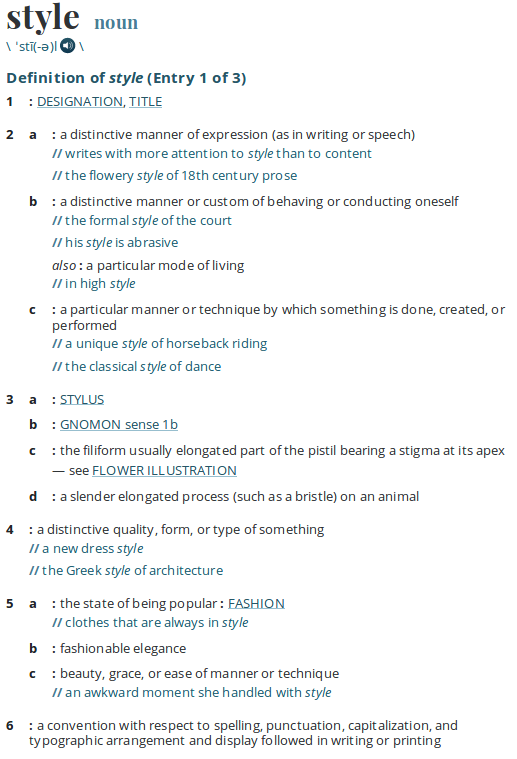
\includegraphics[scale=0.5]{./images/introduction/style_def_webster.png}}
    \caption{Definition of style in Merriam-Webster dictionary}
    \label{fig:style_def_webster}
  \end{figure}

  \begin{itemize}
    \item When we say the word "seriously?". Depending on the manner we say it, it will carry different meaning (sarcastic or surprise for example). One word, two different manners to say it.
    \item Handwriting: You can write down the same the letter (the task), but with multiple typefaces (the style) (figure \ref{fig:different_fonts}).
    \item A movie setting: the script is provided to the actor. There are, however, many ways for the actor to perform what is written in the script, in order to convey different messages/experiences to the audience.
    \item Clothing and fashion: different groups of people have different general style lines -- depending on the region, ethnicity \dots etc --. Within each group, we can see people having diverse styles within this general defining style.
  \end{itemize}

  \begin{figure}[!htbp]
    \begin{center}
      \boxed{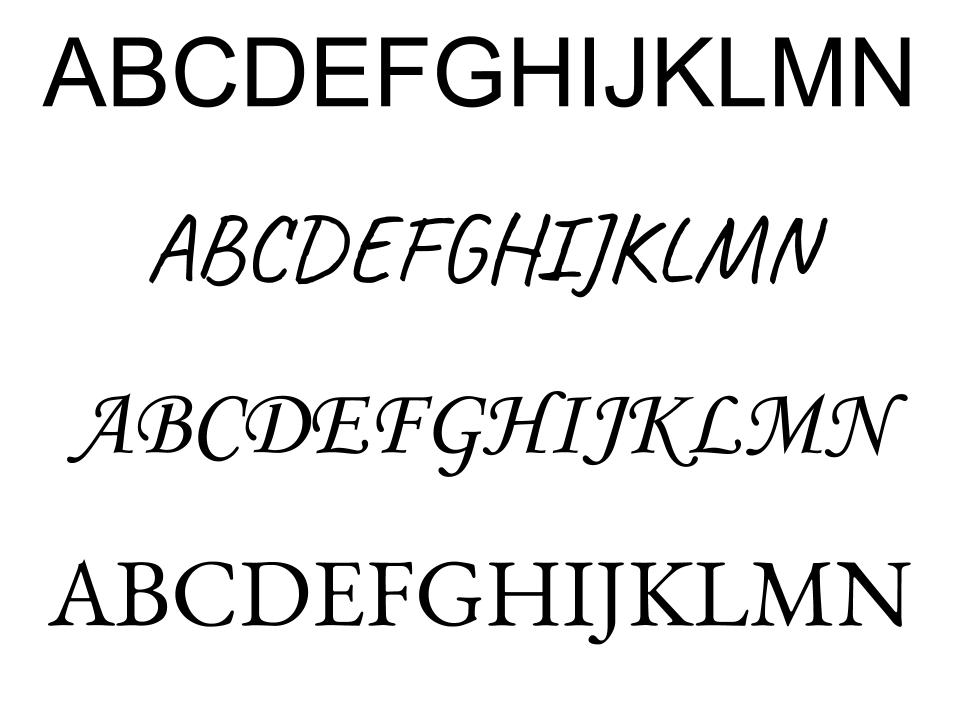
\includegraphics[scale=0.2]{./images/introduction/different_fonts.jpg}}
    \end{center}
    \caption{Multiple styles (different typefaces) for the same letters.}
    \label{fig:different_fonts}
  \end{figure}

  In these two examples, we see a basic structure:
  \begin{itemize}
    \item A fixed part: the word to be said, or the letter identity. We will call this the \textit{content}.
    \item A variable part: the manner we say the word, or the manner we write the letter. We will call this the \textit{style}.
    \item Together, a style and a content forms a \textit{task}.
  \end{itemize}

  \par The mention of styles is quite a lot in the literature in multiple domains, for example:
  \begin{itemize}
    \item \textbf{Speech synthesis}:~\citep{tachibana2004hmm} defines speaking style in a high-level manner, in terms of emotions expressed by the speaker, like 'joy', 'sad', or the interpolation between them, when reading a text.~\citep{wang2018style} looks at the speech style in a more detailed manner, considering different aspects of speech prosody, like the paralinguistic information, intonation and stress.
    \item \textbf{Car driving}: there are multiple ways to categorize the different driving styles. It can be based on the safety aspect~\citep{johnson2011driving}, the aggressiveness of the maneuver~\citep{dorr2014online,xu2015establishing}, the impact on fuel consumption~\citep{manzoni2010driving,neubauer2013accounting}. Many other identification basis for driving styles are summarized nicely in~\citep{martinez2017driving}.
    \item \textbf{Handwriting}: handwriting can be offline (the final image of the letter) or online (recording the movement of the pen/drawing tool). Depending on which one considered, the style profile can change. Figure \ref{fig:different_fonts} is an example of different offline styles (the typefaces). But when we consider the online aspect of the drawing, we can see different aspects, like in figure \ref{fig:online_handwriting_styles}, where we see that the same drawing can be in clockwise or counterclockwise direction (we will expand more on this point in chapter \ref{ch:framework_sec:styleperletter}).
  \end{itemize}

  \begin{figure}[!htbp]
    \centering
    \begin{subfigure}[tb]{0.45\textwidth}
        \boxed{
\includegraphics[width=\textwidth]{images/introduction/DIFFERENCE_IN_STYLE_PERCEPTION_1.jpg}}
        \caption{Offline drawing}
    \end{subfigure}

    \begin{subfigure}[tb]{0.45\textwidth}
        \boxed{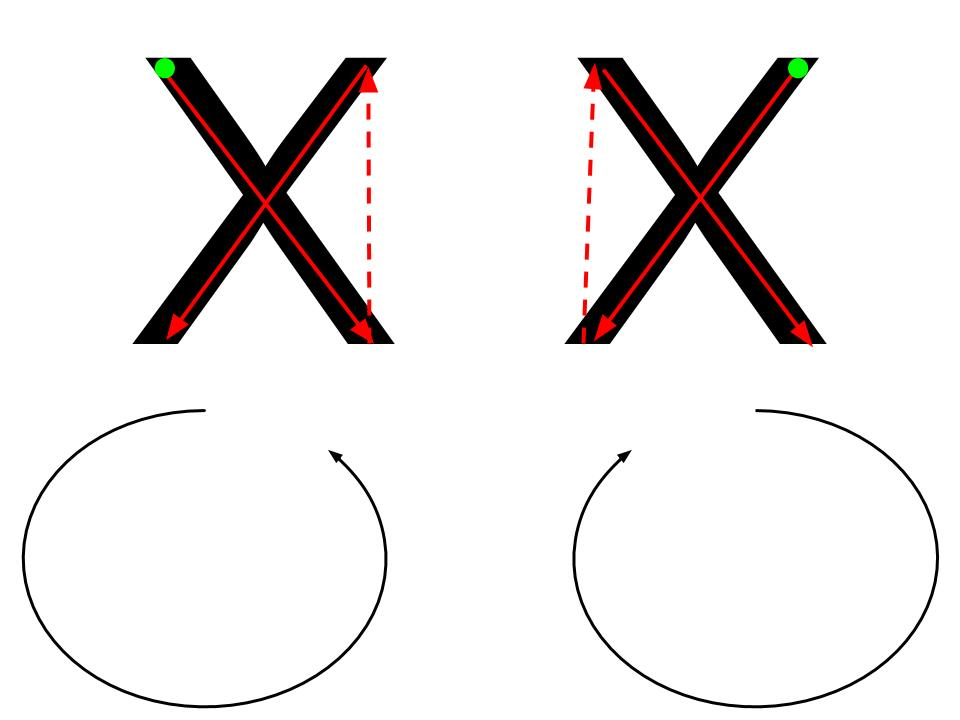
\includegraphics[width=\textwidth]{images/introduction/DIFFERENCE_IN_STYLE_PERCEPTION_2.jpg}}
        \caption{Online drawing}
    \end{subfigure}
    \caption{Example for style in case of online handwriting. Although both examples looks the same when we look at it in the offline mode (the final drawing), they are quite different when we consider the online aspect (the dynamics of the pen when drawing them). Although not illustrated here, it is important to note that some aspects of the online drawing dynamics can be deduced from the offline drawing -- in other words, the dynamics can affect the end result --~\citep{diaz2017recovering}. In this case, the starting point and the direction of drawing (clockwise or counterclockwise) are different. The solid line indicate a stroke, and the dotted line indicate an air stroke (the transition of the pen in the air between two strokes). The green dot is the starting point.}
    \label{fig:online_handwriting_styles}
  \end{figure}

  \par One thing we would like to highlight here: that styles are not thing we all agree on. It can be hierarchical as well. In the clothing example earlier, people are affected by the style group they belong to, but within this cluster, people have diverse individual styles. The same happens in handwriting: education and culture affects the style cluster people belong to, but we can observe a wide range of individual styles in each cluster.

  \par Another thing to highlight is that there is no one definition for styles. It depends on the aspect of interest that we want to observe and study -- in car driving, safety and fuel consumption are two areas of interest, leading to different type of styles --. This leads to an important characteristic of \textit{styles}, that it is an ill-defined concept. We know that \textit{styles} are rich in information and important in communication between humans. They are needed in order to convey meaning. As noted in~\citep{taylor2009text} -- in the context of speech synthesis --, a proper rendering of styles affects the overall perception. However, we can not completely remove the ambiguity in this definition.

% Talk about style in images, speech, handwriting, driving,...etc. Also, distinguish between static and temporal styles.
% \setlist{nolistsep}\begin{itemize}[noitemsep]
%     \item What is a task? what is a style? how both combine to give us an experience?
%     \item Possible scenarios: images, speech, handwriting, autonomous driving
%     \item Style perception depends on 'how you look at it' (the light - angle of view -, body - task - and shadow - the resulting style - example) (cooking rice: no spices or with curcuma. perception: color? taste?) (handwriting: online styles? offline style?). Then end up with the conclusion that styles are ill-defined.
% \end{itemize}


% \section{Why studying styles?}
% \setlist{nolistsep}\begin{itemize}[noitemsep]
%     \item Shortcoming of applying machine learning methods -- average over previous scenarios, doesn't consider styles in advance --.
%     \item HRI example: the need for personalization to enhance the interaction experience.
%     \item Speech example: different utterances change the perceived message
% \end{itemize}



\section{What is the objective of this project?}
\par Our long-term objective is to enable our humanoid iCub robot Nina \ref{fig:nina_robot}, to have a exhibit personalized behavior suitable for the person interacting with it. This will enhance the user experience, and will allow for a more natural interaction with the robot. It is shown that a robot which exhibit a personalized behavior is more likable acceptable by humans, and perceived as an intelligent entity~\citep{churamani2017impact}. Humans have different preferences when interacting with each other, or interacting with the robot, and taking them into account does improve the quality of interaction, and the potential of success for the task~\citep{kashi2018smooth}.

\par At the moment, we successfully used machine learning approaches in order to build models of human-robot interaction~\citep{mihoub2016graphical,bailly:hal-01939223,nguyen:hal-01609535}. However, when using these models to generate behaviors, this behavior usually represents an average over the learned behaviors (which is expected). The goal is to learn models of styles, and use it to bias the models of interaction that we have, in order to generate more personalized behaviors. We want the robot to adapt to the human partner on different levels, and not just act in a reactive manner to the human actions. It has been shown that a suitable cognitive model for human-robot interaction takes into account long term styles -- for example, the person age, gender and if he/she is shy or not --, and short term decision making -- in talking with the human for example --~\citep{thorisson2002natural,bailly2010gaze}. The ability to identify, extract and use the human style traits will enable biasing the robot model to adapt for the human partner.

\begin{figure}[!htbp]
  \begin{center}
    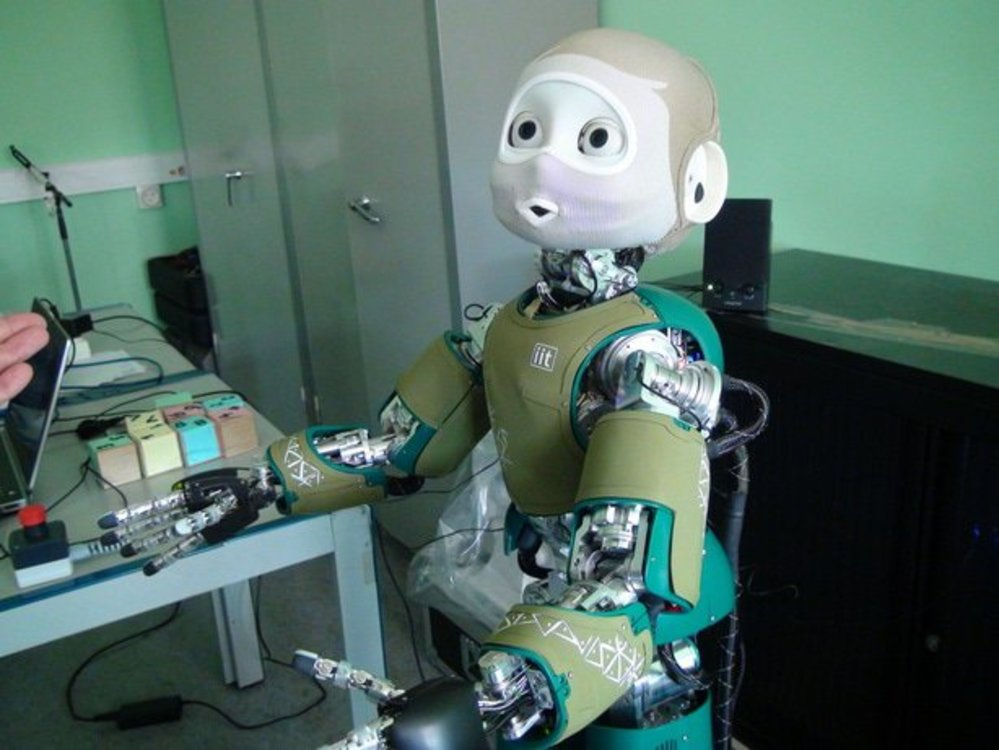
\includegraphics[scale=0.3]{./images/introduction/nina_robot.jpg}
  \end{center}
  \caption{The iCub humanoid robot (Nina).}
  \label{fig:nina_robot}
\end{figure}

\section{Why Handwriting?}
  \par As mentioned earlier, the final objective of this project is to extract and transfer styles in the context of human-robot interaction. What this has to do with handwriting?
  \par The usage of deep learning in HRI is still in its infancy, mainly because of the lack of datasets. The issue is not collecting the data (there are many small open-source datasets available online), but having a unified set of objective and platforms for HRI, which is not an easy challenge. We envision that this problem will be resolved, as there is a growing interest in the community to address it.

  \par Thus come handwriting. We use it as a proxy platform to understand, build and test different approaches to use deep learning. It has many advantages to make it a good proxy, including:

  \begin{itemize}
    \item Availability of datasets: several datasets already exist, with large quantities of data.
    \item Diverse of tasks and styles: there are many tasks (letters) in handwriting, ranging from simple (like letter 'C') to complex (like letter 'E'), and the writers exhibit a diverse set of styles on the different tasks, making handwriting a good candidate to explore the problem of styles.
    \item Several style aspects are accessible to investigate visually, making it more accessible for in-depth analysis, and getting insight on how the model behaves.
    \item Several datasets provide information about the writers, like the age, handiness, gender and the origin. This data is interesting in some aspects of the style problem.
    \item We have a clear idea about the content of each task (the identify of the letter or the shape). Usually, the task is presented to us with the content and the style mixed together. How to disentangle the content from the style is an open question, and the fact the styles is an ill-defined problem makes it more ambiguous. With the assumption that we know the content, we can focus our effort on the styles problem\footnote{We will argue later that the task identity is not necessarily a good representation for the task content.}.
  \end{itemize}
  % A disadvantage of handwriting is the lack of the \textit{human interaction} aspect in handwriting.
  While the subjects are interacting with the environment (the pen, tablet \dots etc) -- which is observed and recorded --, there are no human interaction aspects in this domain of data, which is a disadvantage

\section{What is transfer learning? and why do we need it?}
\par We will discuss transfer learning in more detail in chapter \ref{ch:seat}, but for now, we want to motivate having this as one of the PhD objectives.

\par Transfer of knowledge deals with the problem of leveraging the knowledge learned from one task, to accelerate/improve the learning of a new task. This is a skill human do naturally, for example, if you learn Mathematics, and you want to learn physics, you can easily leverage the knowledge of Mathematics to bootstrap your learning of physics. This, intuitive as it seems, is not straightforward for machine learning models. A change in the distribution of the input to the model leads to significant degradation in the performance of the model~\citep{shimodaira2000improving}.

\par Transfer learning is thus a field of machine learning, concerned with developing algorithms and procedures, to enable the transfer of knowledge between different tasks. So many techniques are available for transfer learning, but there is always a common assumption, that the transfer has the potential of success if the tasks are related (i.e., if there is common knowledge between the tasks), otherwise, a transfer learning can at best lead to no improvement, or even reduce the performance of the new model~\citep{weiss2016survey}.

\par Why do we need transfer learning? We do not always have the availability of large datasets on the tasks that we want. In many cases, the acquisition and/or the annotation of large dataset can be prohibitively expensive. For example:
\begin{itemize}
  \item In robotics~\citep{konidaris2012robot,Konidaris:2012:TRL:2188385.2343689}, collecting data can be quite expensive process, due to hardware limitations from one side, and human limitation as well (in case of human-robot interaction scenarios). In addition, with techniques like reinforcement learning~\citep{sutton2018reinforcement}, where the robot learns by trial and error, the process can be prohibitively slow, with safety concerns sometimes. Also, no data augmentation techniques does exist in the literature for HRI, thus synthesizing extra data is not possible. Thus, we need to be able to transfer the knowledge from the task where we have large amount of data, to a relevant task where we do not have this advantage (figure \ref{fig:illustrate_TL}).
  \item In underwater acoustics~\citep{malfante2018automatic}, an essential task is collecting and cleaning the data about the different fish sounds. This is a tediously manual job, and any change (type of fish, time of the day or place in the ocean) degrades the quality of prediction a lot. Transfer learning can be very useful in this case, to reduce the effort needed to collect, clean and annotate the data.
\end{itemize}

\par What we want to achieve in this thesis is to transfer the styles between different tasks. We hypothesize that, when the tasks are relevant (but different tasks, with different contents), that humans share leverage styles between the different tasks. In case of handwriting for example, we can reuse the strokes that we learn in the uppercase letters in order to learn the lowercase letters and digits. We will test this hypothesis in details in chapter \ref{ch:seat}.

\begin{figure}[!htbp]
  \centering
  \boxed{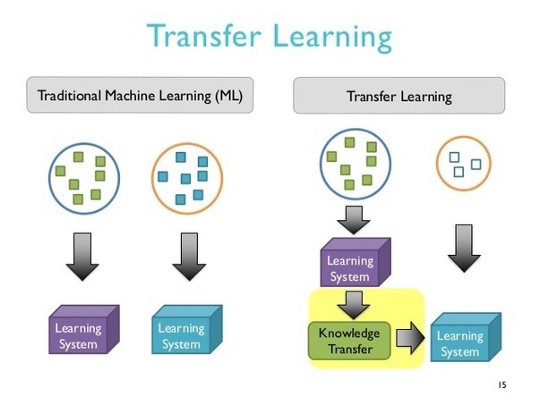
\includegraphics[scale=0.8]{./images/introduction/transfer_learning_illustration.jpeg}}
  % \caption[Transfer Learning Illustration]{Illustration for a practical case of using transfer learning, where we have insufficient data on the new task, and we want to leverage the knowledge learned from another relevant task in order to learn the new task\footnote{Source of this image is \url{https://medium.com/data-science-101/transfer-learning-57ce3b98650}}.}
  \caption{Illustration for a practical case of using transfer learning, where we have insufficient data on the new task, and we want to leverage the knowledge learned from another relevant task in order to learn the new task. Source of this image is~\citep{transimage}.}
  \label{fig:illustrate_TL}
\end{figure}
% \footnotetext{}

\section{If we want transfer learning, why extracting styles?}
  \par It is important not to forget our mission while being consumed by the shiny light of machine learning. It is easy to fall into the trap of "getting the extra 0.1\% accuracy", figure \ref{fig:current_ml_comic}. Extracting styles enables us to have an idea of what the model actually learned (i.e., it makes the model more interpretable). But why do we need interpretability? Many reasons:
  \begin{itemize}
    \item Debugging: Neural networks are notoriously known for being black box models. Extracting styles gives us some indication on what the system learned, and whether it learned relevant information.

    \item Discovery of new things: in the era of big data, trying to reason on the data directly is no longer feasible. Instead, a good approach is to reason on a model that fits these data (i.e., the model compresses the data into fewer dimensions). We would like to use this model to reason and discover new things about the data. After all, \textbf{the goal of science} is to gain knowledge about the world, and an understanding of how it works. One thing we are interested in is to illuminate the workspace of interaction: what are the limits of possible actions, expected reactions and end results. These kind of questions will benefit a lot understanding what the model actually learned.

    \item Understanding why: in some cases (e.g., in case of unexpected events), it is human curiosity to understand the reasoning behind the different decisions. We would like to get insight on why the model led to that particular decision.

    \item Developing safety measures: in many applications (like when dealing with the robots), it is important to be sure that the robot is a 100\% safe for the human. Understanding what the model learned can give us insight on the shortcomings of the model, allowing us to fix or improve.

    \item Social acceptance: humans always tries to attribute beliefs, intentions, personality traits and desires to different objects~\citep{heider1944experimental}. An interpretable machine will reinforce these sensations in humans.

    \item Improve social interactions: when the robot can explain itself and its perception of the world, it creates a common understanding with the human. This allows the humans to build a mental model for what the robot is actually trying to do, thus, building trust between humans and the robot.
  \end{itemize}

  \par For further details, we strongly recommend the book~\citep{molnar2019} on the topic of machine learning interpretability.

  \begin{figure}[!htbp]
    \centering
    \boxed{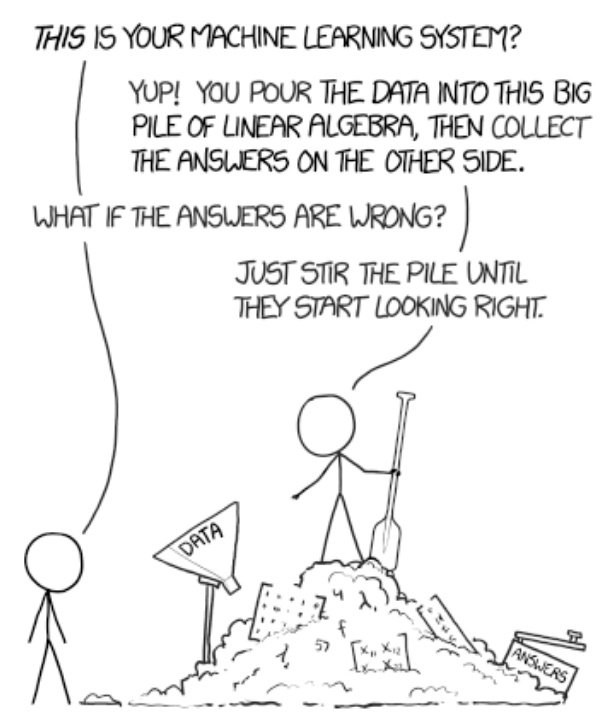
\includegraphics[scale=0.5]{images/introduction/current_ml_tradition.png}}
    \caption{Source: \url{https://xkcd.com/}}
    \label{fig:current_ml_comic}
  \end{figure}


\section{Contributions of this PhD}
\par In this manuscript, we discuss the different contribution of this PhD, addressing different aspects of the styles:
\begin{enumerate}
  \item Propose a manner of thinking about styles: traditionally, a lot of work has been done in order to manually extract and annotate styles, and deal with styles in terms of predictability (using the extracting styles in a regression/classification problem). In this PhD, we propose to implicitly evaluate styles by observing the generative aspects of the model (letting the model generates behaviors, and trying to evaluate the distance between these behaviors and the target/ground truth ones). This is discussed in chapter \ref{ch:GBEM}.
  \item Propose and build benchmarks and evaluation metrics, and ground those metrics, in order to compare and evaluate future style extraction methods. This is discussed in chapter \ref{ch:GBEM}.
  \item Propose a generic framework to study styles, using a conditioned-autoencoder. We evaluate this framework in its basic form against the benchmarks. We further validate this framework by extracting verbose styles from it, including ones that are not known from the literature. This is discussed in chapter \ref{ch:framework}.
  \item Last, we address the problem of style transfer. We show how to use our proposed framework in order to transfer styles. We perform extensive experiments in a lot of combinations of tasks, on two different datasets. We also enhance and expand on the evaluation metrics we use in order to quantify the quality of transfer. This is discussed in chapter \ref{ch:seat}.
\end{enumerate}
% Some informal contributions are: \textbf{not sure about this section}
% \begin{enumerate}
%   \item Definition of styles??
% \end{enumerate}

% \section{An overview of the manuscript}
% \par The main contribution of the PhD is a thinking framework to study and observe styles, in the temporal case, using neural networks, while the task is defined beforehand. Through implementation, benchmarks and evaluation, and analysis of the networks performance (and sometimes its behavior), we seek to provide support to ground this framework, and our hypotheses about it.
%
% \par The most general elements/components has been used in our study, in order not to couple the effect of more advanced/complicated items with our conclusions. This leaves a big room for further improvements and exploration as well.
%
% \par Using machine learning as tool enables us to process large amount of data.

\section{Thesis outlines}
\par We start in chapter \ref{ch:dataset} by explaining the datasets used in this PhD, and explore their different characteristics, and the preprocessing performed on them. In chapter \ref{ch:GBEM}, we discuss first the different aspect of deep learning that we are using in this PhD. We then discuss the different benchmarks and evaluation metrics we propose, and how can we ground them.

\par Once this step is done, it paves the way to discuss our proposed framework to study styles in chapter \ref{ch:framework}. We start first by presenting the relevant literature, then move on to the experimental part, where we show the performance of the proposed framework relative to the benchmarks. We conclude this chapter by a section on style extraction, where we shade some light on what the model actually learned.

\par With the elements in place, we can explore the topic of style transfer, in chapter \ref{ch:seat}. As usual, we study with literature over transfer learning, followed by the proposed experiments in order address our hypotheses. We perform a wide range of experiments, to solidify our conclusions about style transfer. We also discuss another possibility to interpret what the model actually learned in section \ref{ch:seat_sec:rf}.

\par We conclude the manuscript by a general discussion over this thesis (chapter \ref{ch:discussion}), the difficulties it faced, and the possible future research directions based on the results. We believe that this thesis answered multiple questions, but it also created more questions and research interests for further investigation. We then make a short summary and conclusions about the work done in this thesis in chapter \ref{ch:closing_remarks}.

% \theendnotes
% \setcounter{endnote}{0}

% \theendnotes
% \setcounter{endnote}{0}

\chapter{Datasets}
\minitoc% Creating an actual minitoc

\section{Introduction}
\par In order to test the different hypotheses and ideas presented in the introduction chapter, we need to select suitable domain to carry out the experiments, which determined by the data. The choice of the data is a selection between different trade-offs: relevance (i.e., it contains the relevant information to perform the study) VS readiness of the data (i.e., is it already available? and how expensive it is to acquire the data?), simplicity VS realism (simple data has less noise and less irrelevant patterns, but the ability to handle realistic data provides stronger support for the hypothesis), and the amount of data available.

\par It is traditional in the machine learning community to use two or more datasets to address the questions. This way, it is possible to detect issues like having a very specific method that work only in a limited context\sidenote{This is not wrong in itself, it depends on the objective of the work. In our case, we want to show an indication that our methods can generalize.}, and to avoid the effect of unknown contributing variables.

\par We settled on the domain of handwriting and drawing \textbf{Remeber to explain the reasoning for this choice in the introduction}. In this chapter we present two datasets: Online english letters handwriting dataset, \textit{IRONOFF}, and online sketch drawing dataset, \textit{Quick Draw!}. We present general information and exploratory statistics about both datasets, and discuss the categories/tasks in each dataset, and argue why both datasets are suitable for this study.

\begin{mdframed}[backgroundcolor=blue!20]
    \begin{center}
        Points addressed in this chapter
    \end{center}

    \setlist{nolistsep}
    \begin{itemize}[noitemsep]
        \item Present \textit{IRONOFF} handwriting dataset.
        \item Present \textit{QuickDraw!} sketch drawing dataset.
        \item Motivate the suitability of these datasets for this study.
    \end{itemize}
\end{mdframed}

% \setlist{nolistsep}
% \begin{itemize}[noitemsep]
%     \item Write something about the reasoning behind choosing each dataset. IRONOFF has diversity of styles, but clear semantics for each task -- most of the time --. QuickDraw is more chaotic, the task semantics are not well perceived by the different contributors.
% \end{itemize}

\section{Online Handwriting -- \textit{IRONOFF}}

\par \textit{IRONOFF} \citep{791823} is a cursive handwriting dataset provides us with isolated letters, thus allowing us to focus on the problem of styles with a reasonable complexity, and gives us the advantage that the content of the task is well known beforehand (i.e, the identity of the letter). Other cursive handwriting datasets do exist, like \textit{IAM Handwriting Database} \citep{marti1999full}. However, they use whole sentences/paragraphs, instead of individual letter, thus making the problem more complicated.

Basic information about \textit{IRONOFF} dataset as a whole:
\setlist{nolistsep}
\begin{itemize}[noitemsep]
    \item Around 700 writers in total. We use the 412 writers who have written isolated letters.
    \item 10,685 isolated lower case letters, 10,679 isolated upper case letters, 4,086 isolated digits and 410 euro signs.
    \item The gender, handiness, age and nationality of the writers.
    \item For each writer/task (letter or digit) example, we have that example's image - with size around ~167x214 pixels, and a resolution of 300 dpi -, pen movement timed sequence comprising continuous X, Y and pen pressure, and also discrete pen state. This data is sampled at 100 points per seconds on a Wacom UltraPad A4. Figure \ref{fig:ironoff_example} shows an example for format of the the provided data.
\end{itemize}

\par We explored the information available about the writers in the dataset (see figure \ref{fig:ironoff_basic_stats}), we can see that almost all the participants are of French nationality, and majority of them are less than 30 years old. The data is almost balanced between males and females, but largely unbalanced between left and right handed people. This indicates that this dataset is not a representative for all the people. This, however, does not limit our study (a fair representation for all the people is not a point of concern).

\par We then explored the handwriting examples from multiple points of view. In figure \ref{fig:ironoff_strokes}, we can see the frequency of strokes for different tasks. We can see that letters like \textit{C} and \textit{L} needs one stroke only, while \textit{I} and \textit{E} requires the most number of strokes in order to draw properly. By combining this with observation about the drawing time for different tasks (see figure \ref{fig:ironoff_drawingtime}) and the pausing time (see figure \ref{fig:ironoff_pausingtime}), we can have a good indication about the complexity of each task relative to the other tasks. The more strokes the task has, the more drawing and pausing time is needed, and the more complex the task is.

\par One challenging issue with this dataset however is that we have only one example for each writer-letter combination. This makes the task more difficult, because it is hard to extract a writer style using very few items (the 26 letters/writer in this case).

\begin{figure}[!htbp]
    \centering
    \begin{subfigure}{0.45\textwidth}
        \boxed{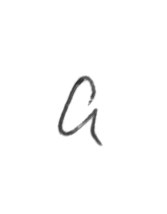
\includegraphics[scale=1.0]{images/dataset/B1_a.png}}
    \end{subfigure}
    ~
    \begin{subfigure}{0.45\textwidth}
        \boxed{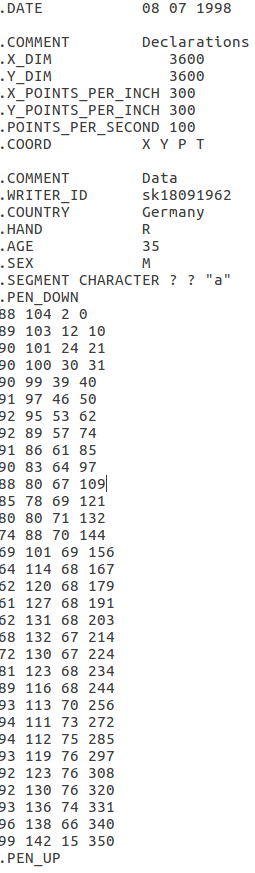
\includegraphics[scale=0.5]{images/dataset/ironoff_file_example.png}}
    \end{subfigure}
    ~
    \caption{An example from \textit{IRONOFF} (letter 'a'). To the left, we have the image of the letter (i.e., offline-handwriting). To the right is an example of the format for the online-handwriting. We have the writer's ID, origin, handiness, age and gender. The sequence of pen movement to draw the letter are then given: pen state (PEN\_DOWN, PEN\_UP), X, Y coordinates, pen pressure, and time.}
    \label{fig:ironoff_example}
\end{figure}

% Omar TODO: crop these images, then they cover part of the header
\begin{sidewaysfigure}[!htbp]
    \centering
    \begin{subfigure}{0.45\textwidth}
        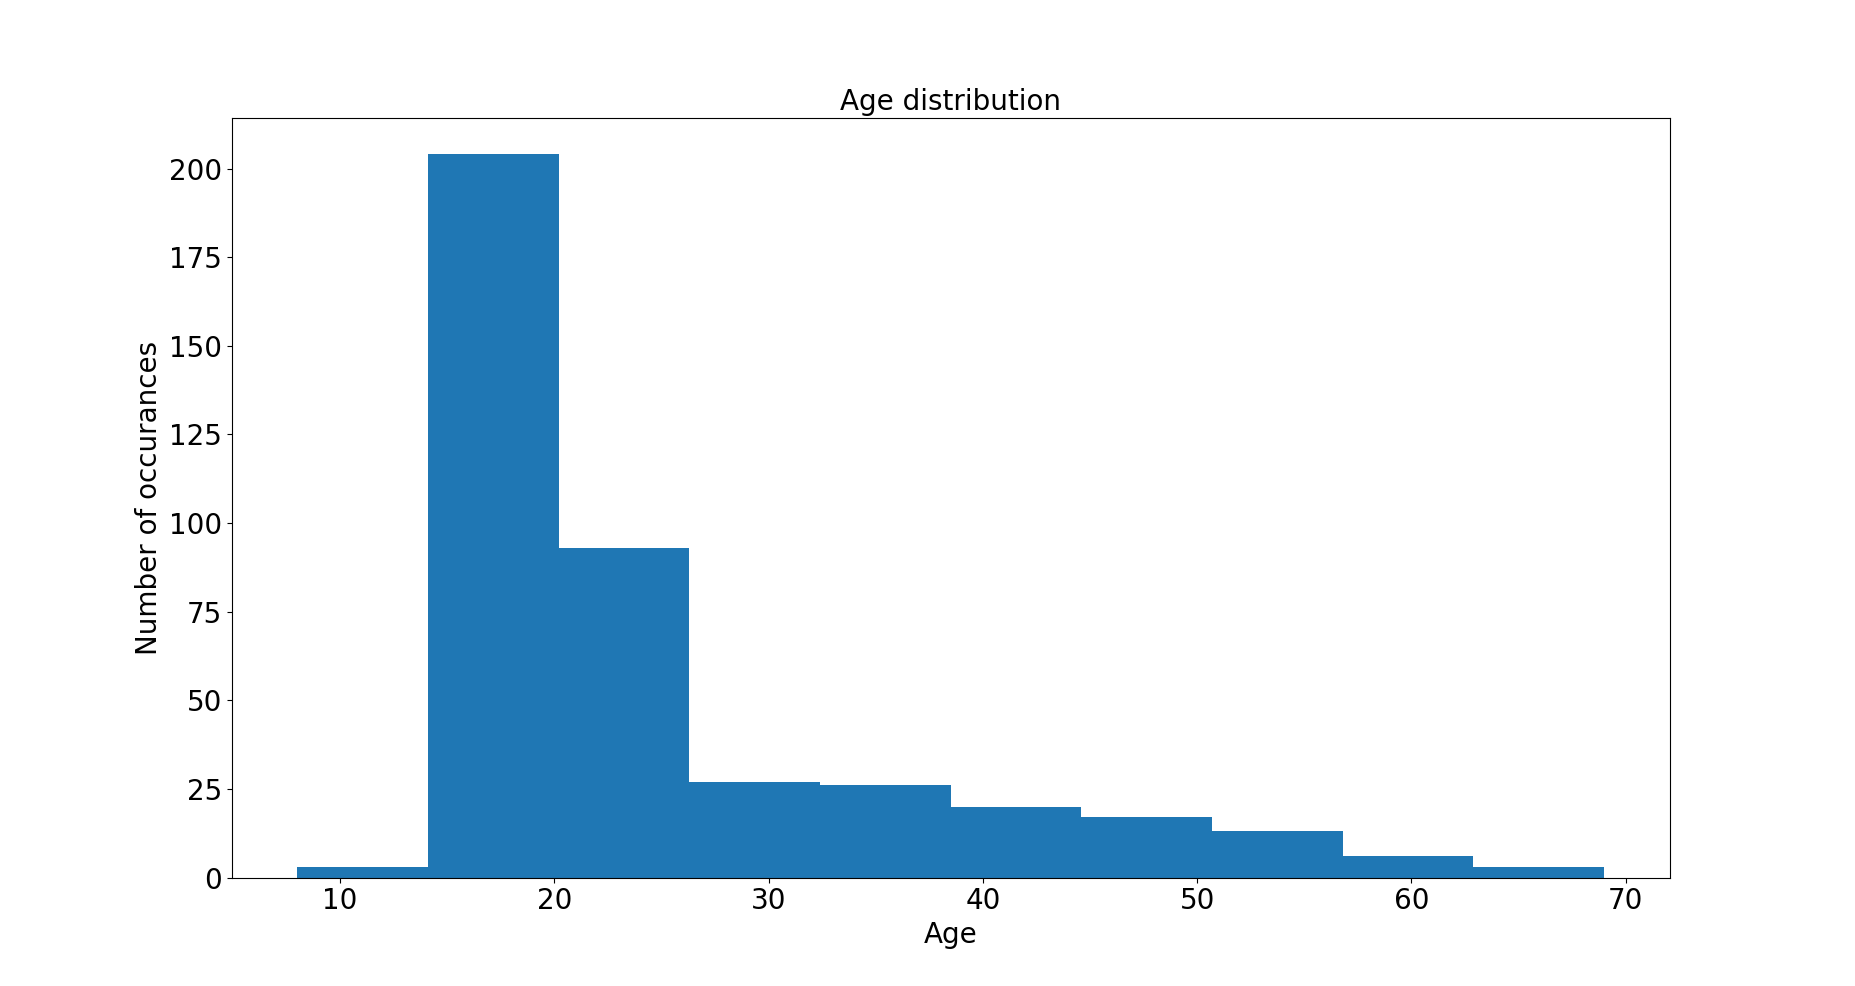
\includegraphics[scale=0.25]{images/dataset/age_dist.png}
    \end{subfigure}
    ~
    \begin{subfigure}{0.45\textwidth}
        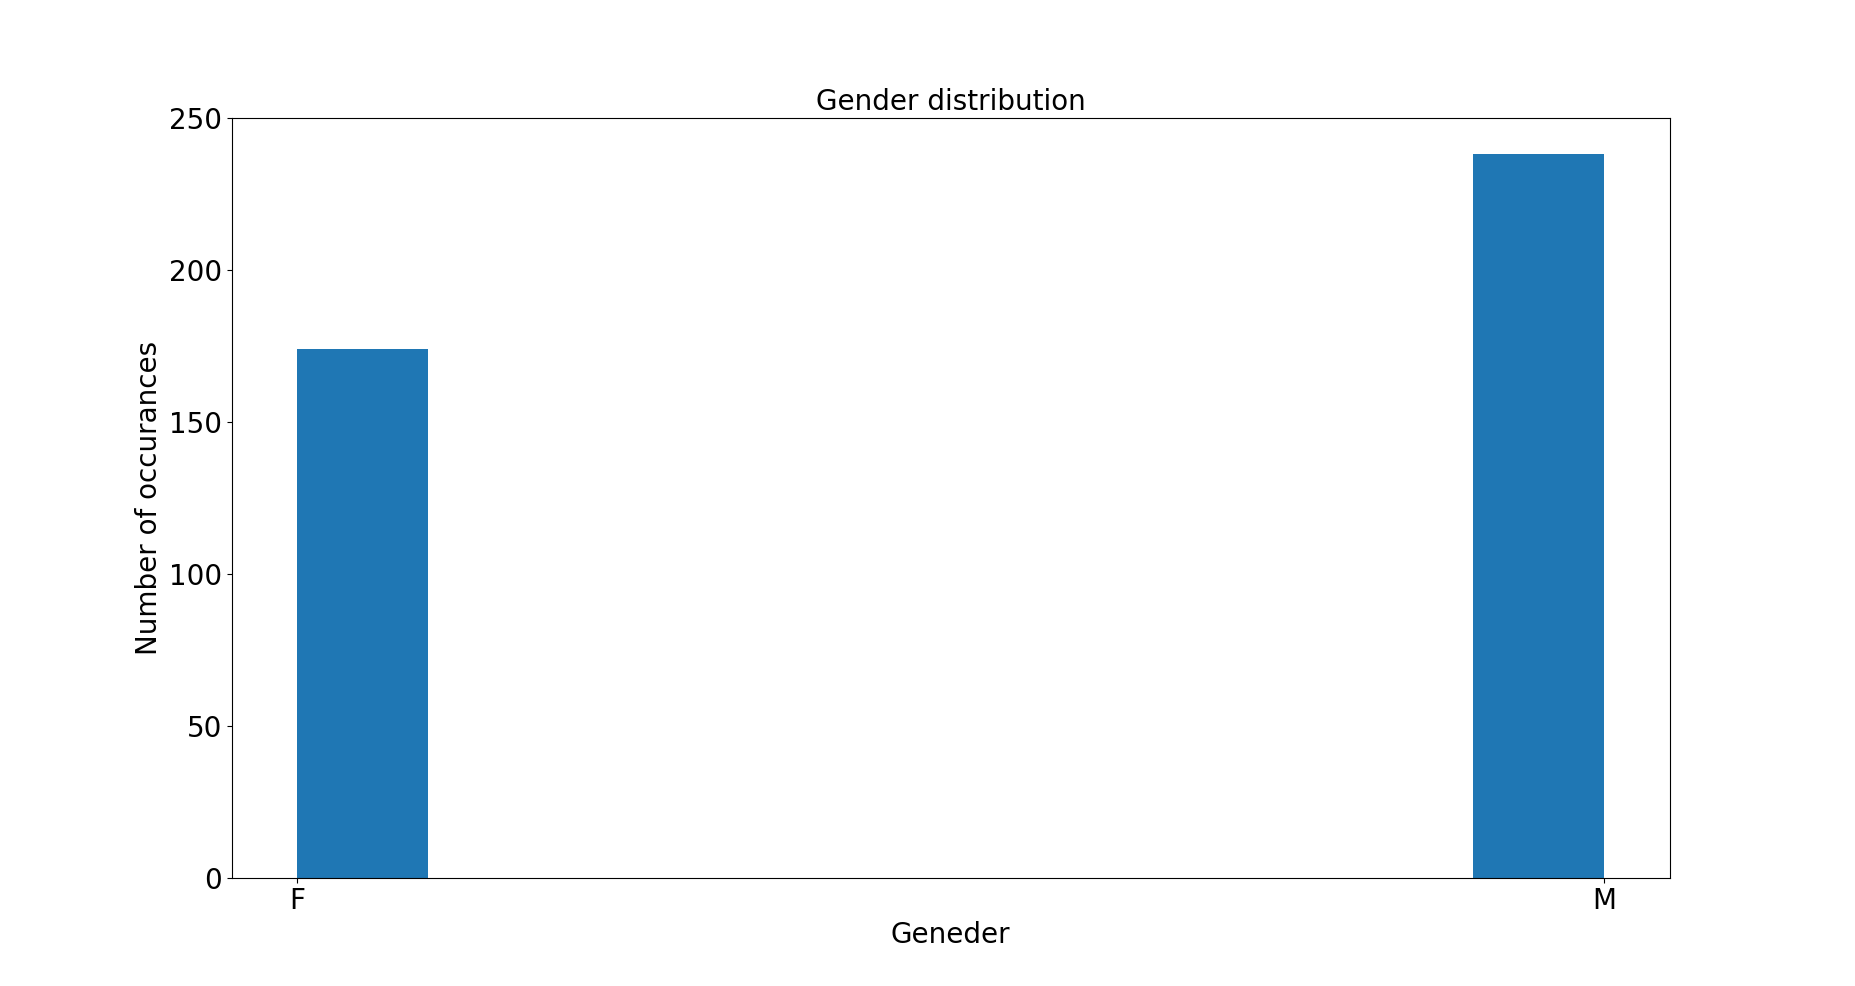
\includegraphics[scale=0.25]{images/dataset/sex_dist.png}
    \end{subfigure}
    ~
    \begin{subfigure}{0.45\textwidth}
        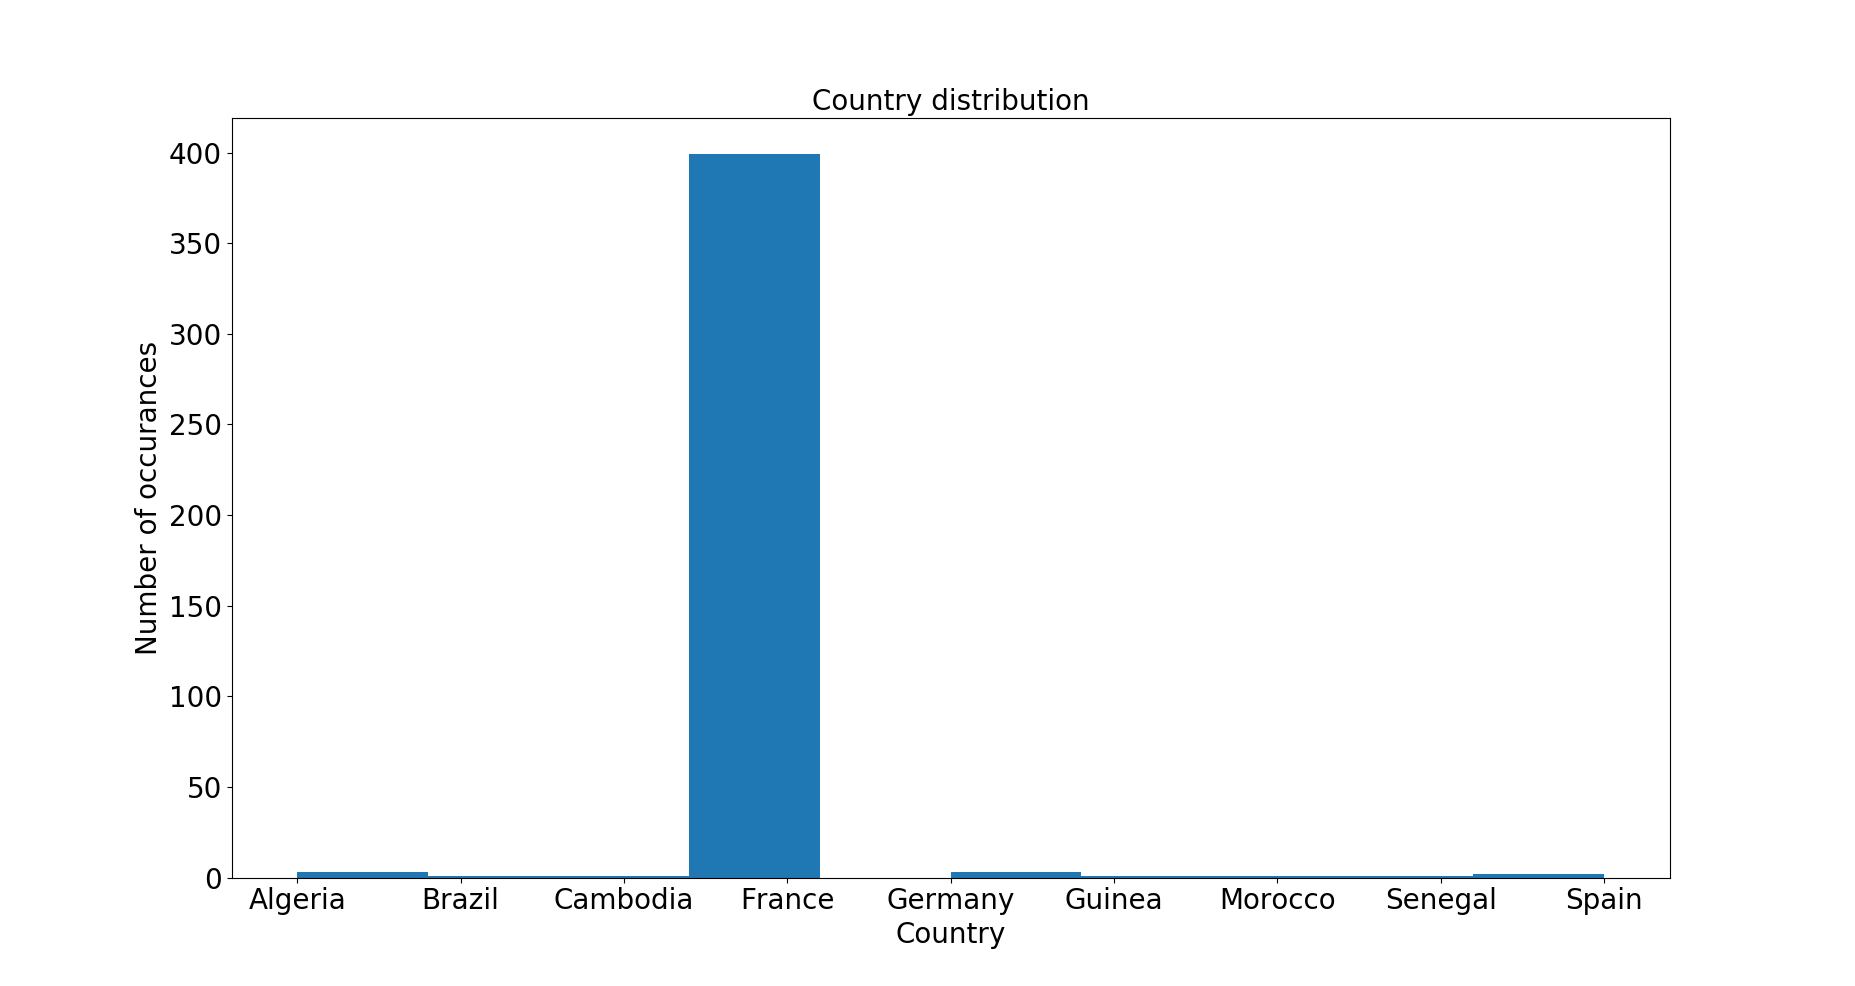
\includegraphics[scale=0.25]{images/dataset/country.png}
    \end{subfigure}
    ~
    \begin{subfigure}{0.45\textwidth}
        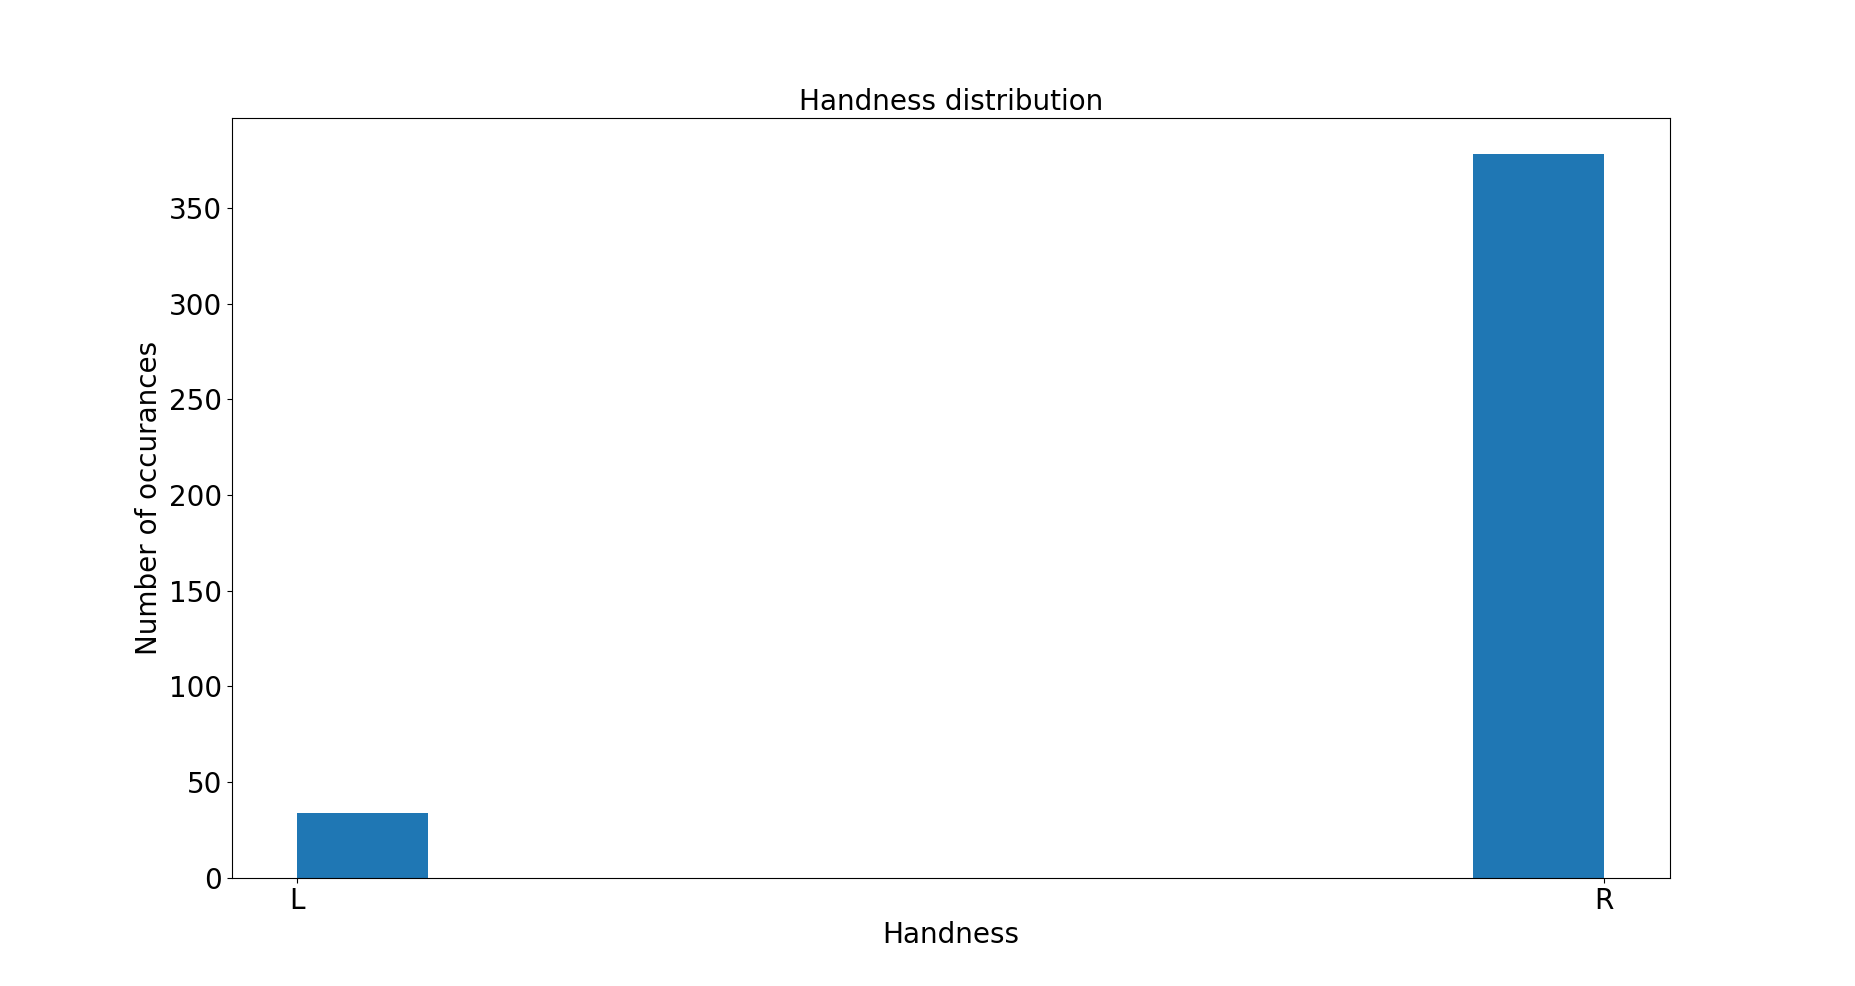
\includegraphics[scale=0.25]{images/dataset/handness_dist.png}
    \end{subfigure}
    ~
    \caption{Summary statistics about the writers in \textit{IRONOFF}: the age, gender, country and handiness.}
    \label{fig:ironoff_basic_stats}
\end{sidewaysfigure}

\begin{sidewaysfigure}[!htbp]
    \centering
    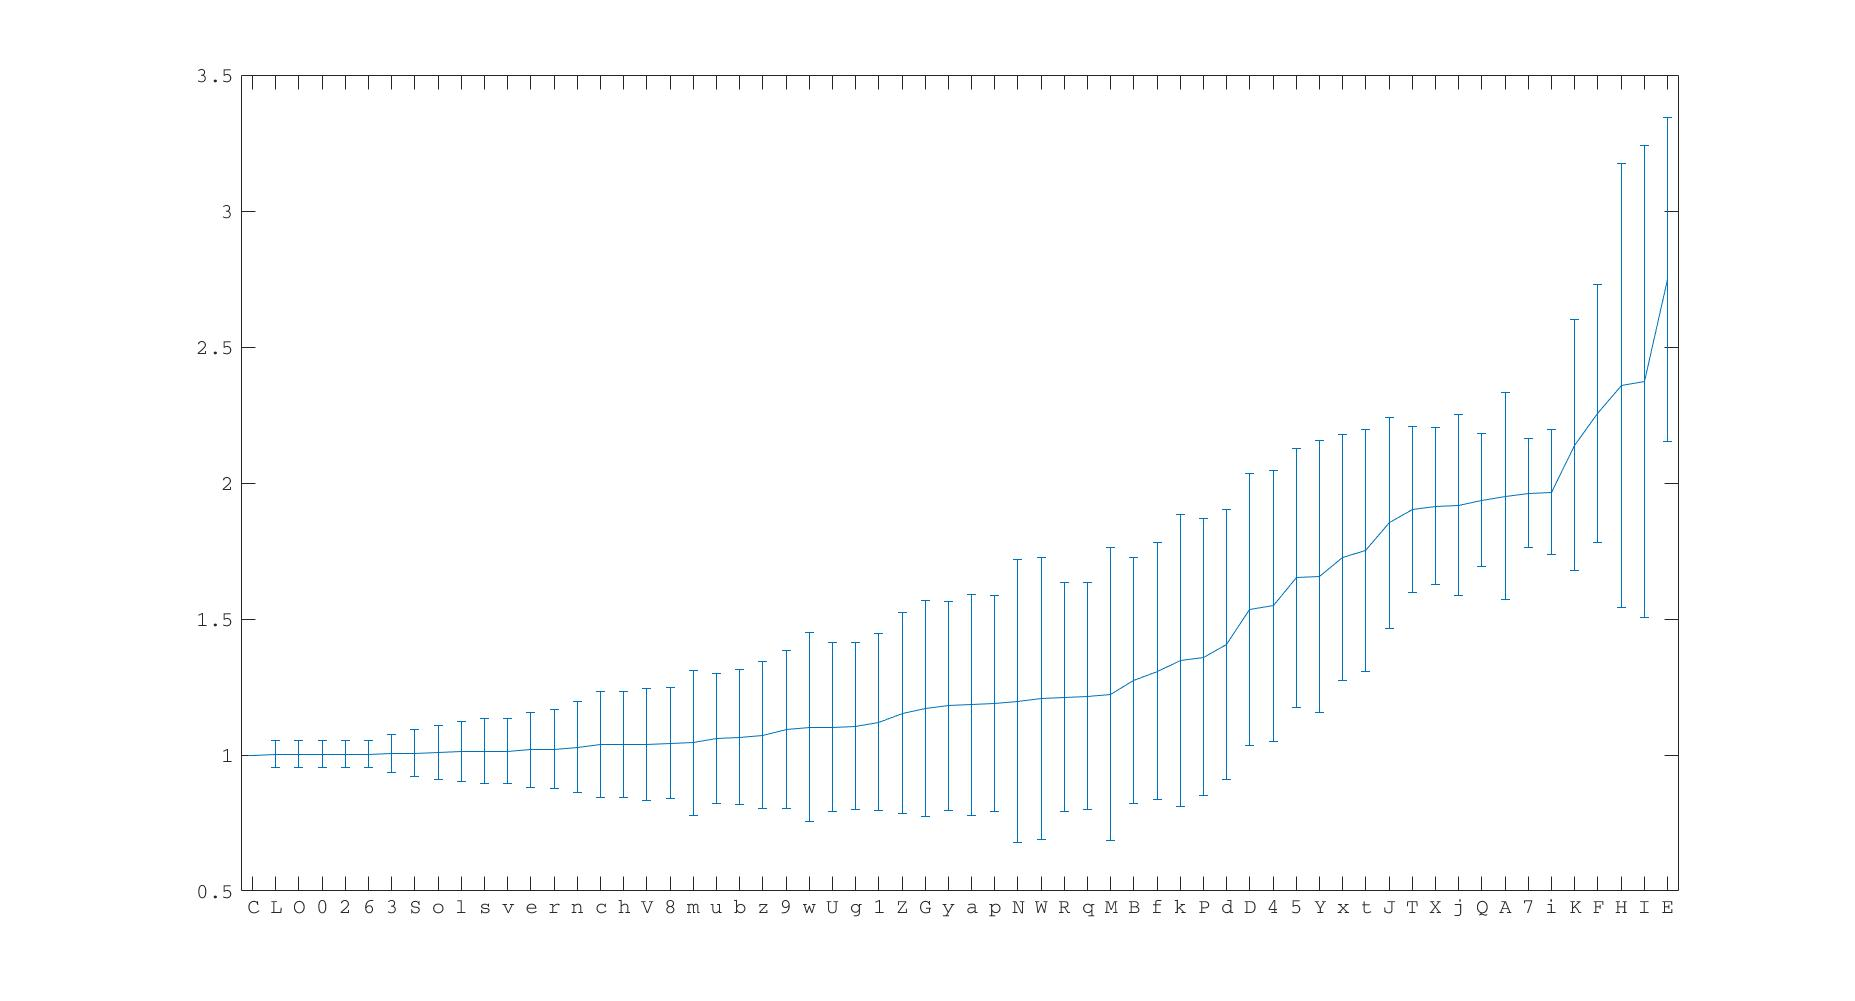
\includegraphics[scale=0.32]{images/dataset/ironoff_strokes.jpg}
    \caption{Summary statistics strokes for all categories in \textit{IRONOFF} dataset (uppercase and lowercase letters, and digits), starting from the simplest to the more complex.}
    \label{fig:ironoff_strokes}
\end{sidewaysfigure}

\begin{sidewaysfigure}[!htbp]
    \centering
    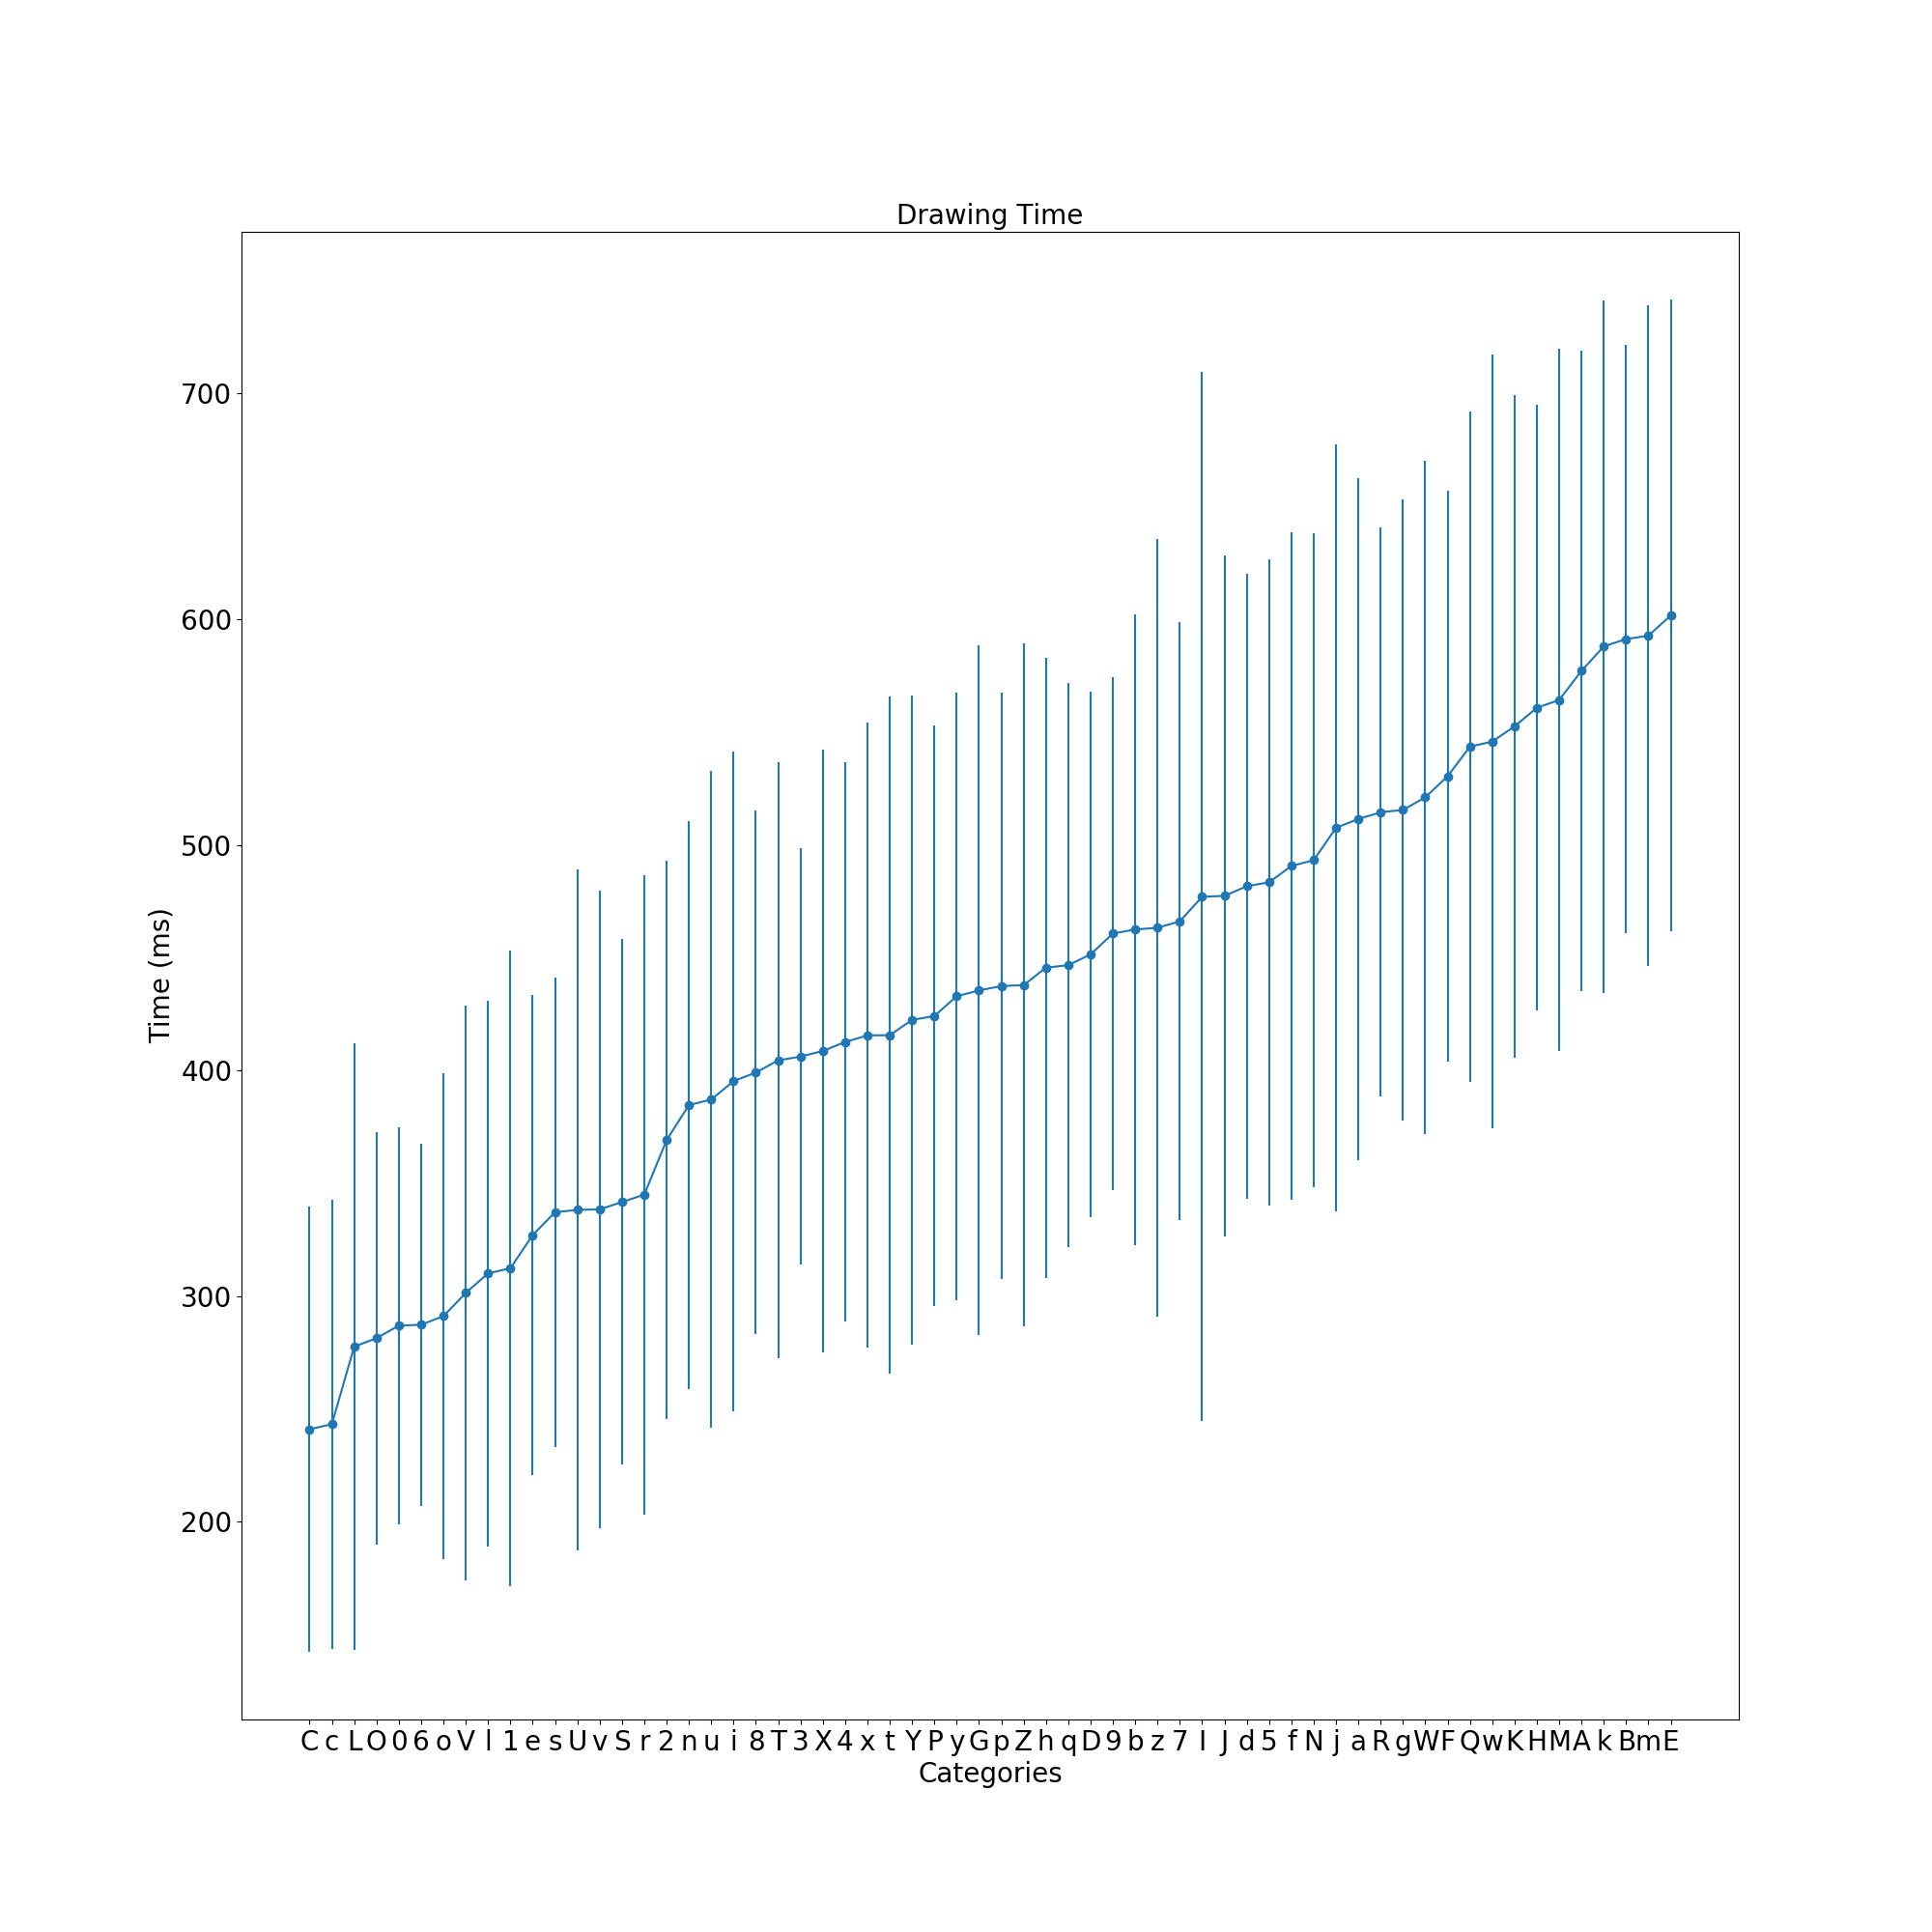
\includegraphics[scale=0.4]{images/dataset/drawing_time.png}
    \caption{Drawing time for all categories in \textit{IRONOFF} dataset, arranged from the smallest to the largest.}
    \label{fig:ironoff_drawingtime}
\end{sidewaysfigure}

\begin{sidewaysfigure}[!htbp]
    \centering
    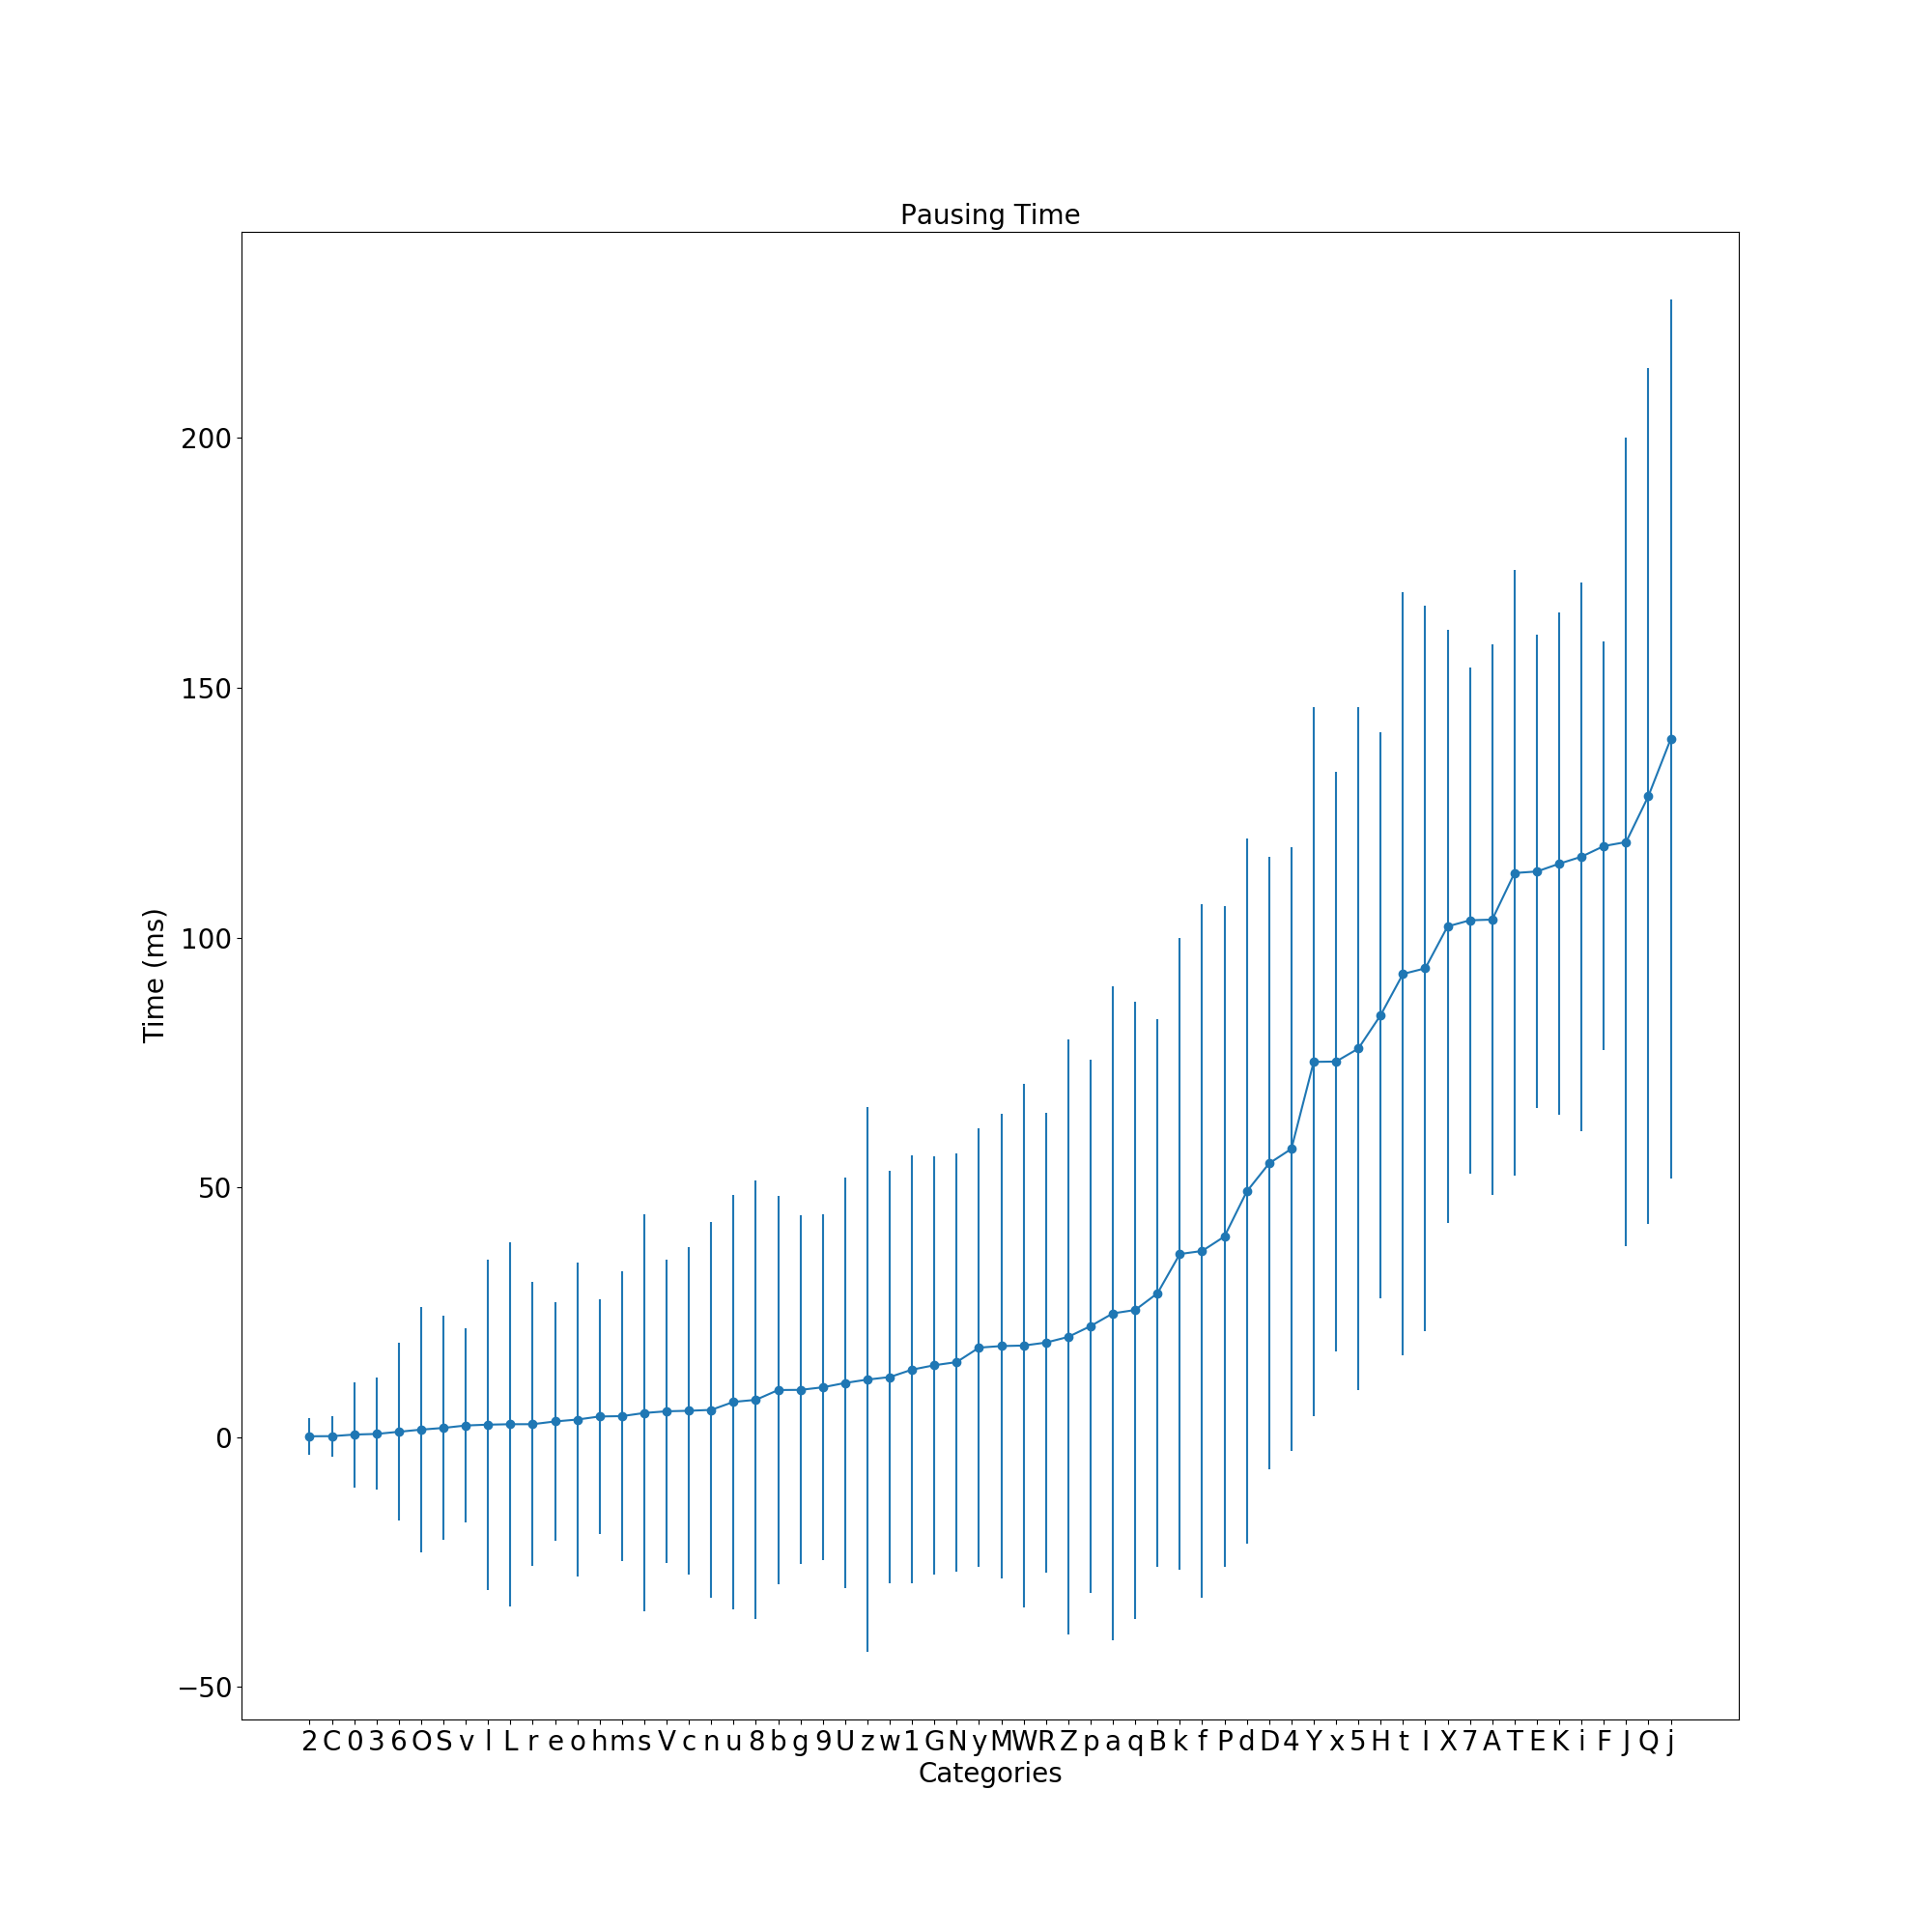
\includegraphics[scale=0.4]{images/dataset/pausing_time.png}
    \caption{Pausing time for all categories in \textit{IRONOFF} dataset, arranged from the smallest to the largest.}
    \label{fig:ironoff_pausingtime}
\end{sidewaysfigure}

\section{Sketch Drawing -- \textit{QuickDraw!}}
\par Around 50 million drawings have been collected by players of the game \textit{Quick, Draw!} \citep{quickdrawgame}, where players are asked to draw one of 345 categories, and a neural network tries to classify the drawings into the right categories. With more data collected and labelled, the network gets better (it learns from the flagged errors). The collected dataset is available online for free \citep{quickdraw}. Example of the shapes collected are in figure \ref{fig:quickdraw_preview}.

\begin{sidewaysfigure}[!htbp]
    \centering
    \boxed{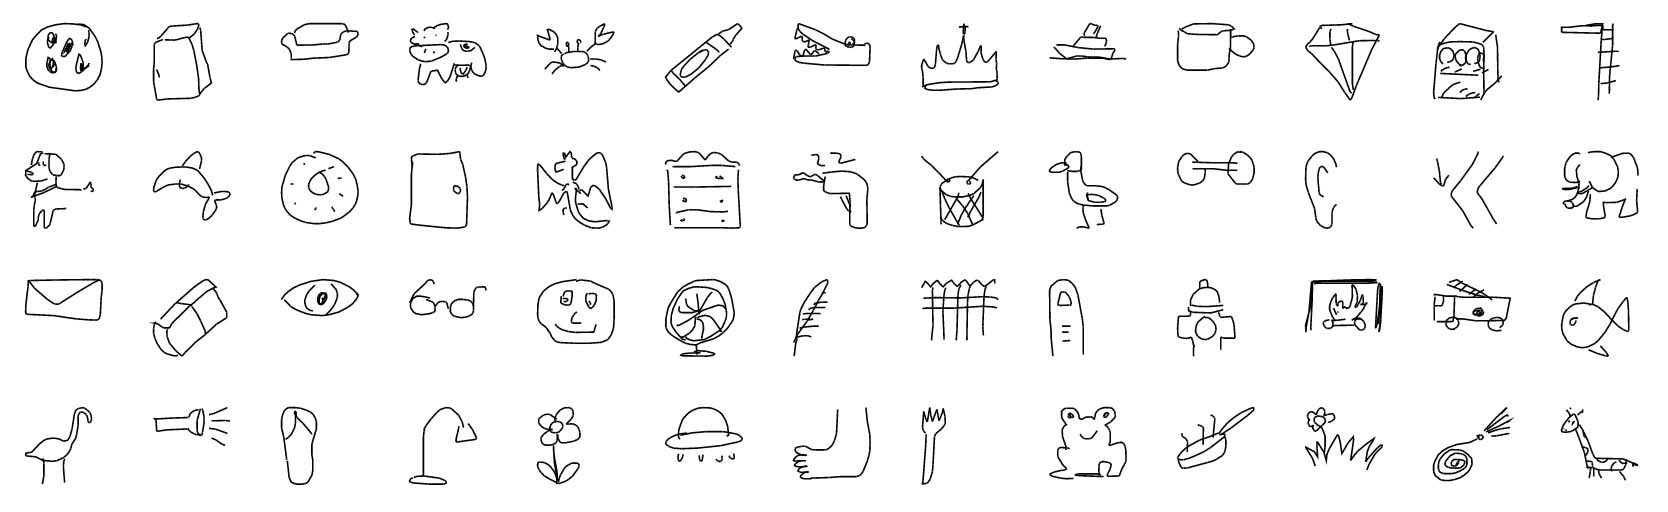
\includegraphics[scale=0.7]{images/dataset/quickdraw_preview.jpg}}
    \caption{Examples from different categories in \textit{QuickDraw!} dataset. Source of the images are \citep{quickdraw}}
    \label{fig:quickdraw_preview}
\end{sidewaysfigure}


\par Each sample in the dataset contains the following data:
\setlist{nolistsep}
\begin{itemize}[noitemsep]
    \item key\_id: a unique identifier for this sample.
    \item word: the category the player was asked to draw.
    \item recognized: if the neural network in the game did recognize the drawing as part of this category.
    \item timestamp: to mark the creation time of the drawing.
    \item countrycode: the location of the player when the drawing was made.
    \item drawing: an array containing the $X$, $Y$ trajectories, and the time $T$ for each point in the trajectory. Points belonging to each stroke are grouped together.
\end{itemize}

\par In order to focus on the styles aspect, we decided to focus on 5 categories: circle, triangle, square, hexagon and octagon. Our reasoning is that the more complex the task gets (cats for example), it is harder to have a subjective opinion about the styles, and hard to give insights about the results. This is not a limitation on the methods we are proposing though.

\par We sampled 20K samples from each task to perform exploratory analysis on them. In terms of strokes (see figure \ref{fig:quickdraw_strokes}), we can see that there is a large variance surrounding the mean of each category. This trend continues when we look at the drawing time (see figure \ref{fig:quickdraw_drawing_time}) and the pausing time (see figure \ref{fig:quickdraw_pausing_time}). In the sample we analyzed, there are players from around 160 countries, figure \ref{fig:quickdraw_countries}. This is one indication to the increasing complexity \textit{QuickDraw!} dataset presents in compare of \textit{IRONOFF} dataset. \textbf{Put the country distribution in the dataset.}

\par Not all examples are recognizable during the game though. In many cases, the players do not draw the required shape, or draw something quite complicated. The results of the recognition can be seen in figure ~\ref{fig:recognition}, with the relation between number of strokes and length of the drawing. We can conclude that, for the selected categories, the more complex the drawing is (more length or more strokes), the less likely it is to become a recognizable drawing.

\par This dataset is considerably more challenging than \textit{IRONOFF}, for several reasons:
\setlist{nolistsep}
\begin{itemize}[noitemsep]
    \item Even though the players are asked to perform a particular task (draw a circle for example), in several cases, there is no clear resemblance between the drawing and task (e.g., when drawing an octagon, a lot of the recognized drawings do not really resemble an octagon).
    \item The players used a mouse in order to perform the drawing\sidenote{Although there is no reporting about the tools used in the drawing, it is a valid assumption to assume that the mouse is the main tool. }. This sometimes lead to weird behaviours in terms of speed of movement (too slow, too fast), and the number of strokes (players sometimes tend to simplify complex shape, by drawing the whole shape in one stroke, and sometimes they spend too much time to draw it well, with too many strokes).

    This is unlike handwriting, where the writers usually tend to follow some rules (\citep{seraphin2019analyzing}), which is not mostly the case in this dataset.

    \item Thus, some extra parts of pre-processing will need to be added in order to reduce the reduce these effects of the mouse, and make the data more closer to handwriting behavior.
    % \item The choices made in the pre-processing are vital. A basic pre-processing (similar to \textit{IRONOFF}) can still give a lot of variety to learn, which make the learning task challenging. However, with a shape classification in mind, one can be tempted to smooth the shapes and introduce extra about the strokes - for example -, which make the task easier to learn, but not challenging enough to test transfer learning on it.

    \item As mentioned earlier, the variance for each of the selected categories in this dataset is considerable higher than \textit{IRONOFF}.
\end{itemize}

% \par Since the study of styles is challenging, we decided to go for basic/elementary shapes. We selected: circle, triangle, square, hexagon and octagon -- this is also a tricky choice, since if the shapes are too easy, the benefit of transfer learning will not be noticed --.

\par Since these drawings are done using the mouse, an interesting aspect for the recognizable images is the simplicity of strokes used -- easier for player -- (see figure \ref{fig:quickdraw_strokes}). If a pen is used in the drawings, this particular behaviour would not observed. For example, in case of hexagon and octagon, one can expect a higher density on the 6 and 8 strokes respectively, and much less on 1 stroke. Our observation is that it is easier with the mouse to draw the whole shape with one (or few) strokes only. This has two consequences:
\setlist{nolistsep}
\begin{itemize}[noitemsep]
    \item It is difficult to generate the strokes: One/few strokes means that a direct stroke representation is quite sparse (if the length of the shape sequence is 200 time steps, then among all the zeros (199 zeros, representing the current stroke), there is a single 1 value (representing the end of the stroke). This problem has also been noted in the work done in \citep{ha2017neural}, and it is a challenging task to tackle.
    \item Unlike in \textit{IRONOFF} dataset, where the strokes is a contributing feature in identifying the letter and the rules of drawing it, the strokes are not expected to play the same rule in \textit{QuickDraw} -- unless further processing is done --.
\end{itemize}

\par For each class, we randomly -- without replacement -- sampled only from the recognized drawing, traces with less than 200 time step long. ~2K samples (total is ~10K samples). 1K is used for test, 900 for validation, and the rest is the training data.

\begin{sidewaysfigure}[!htbp]
% \begin{figure}[!htbp]
    \centering
    \begin{subfigure}{0.3\textwidth}
        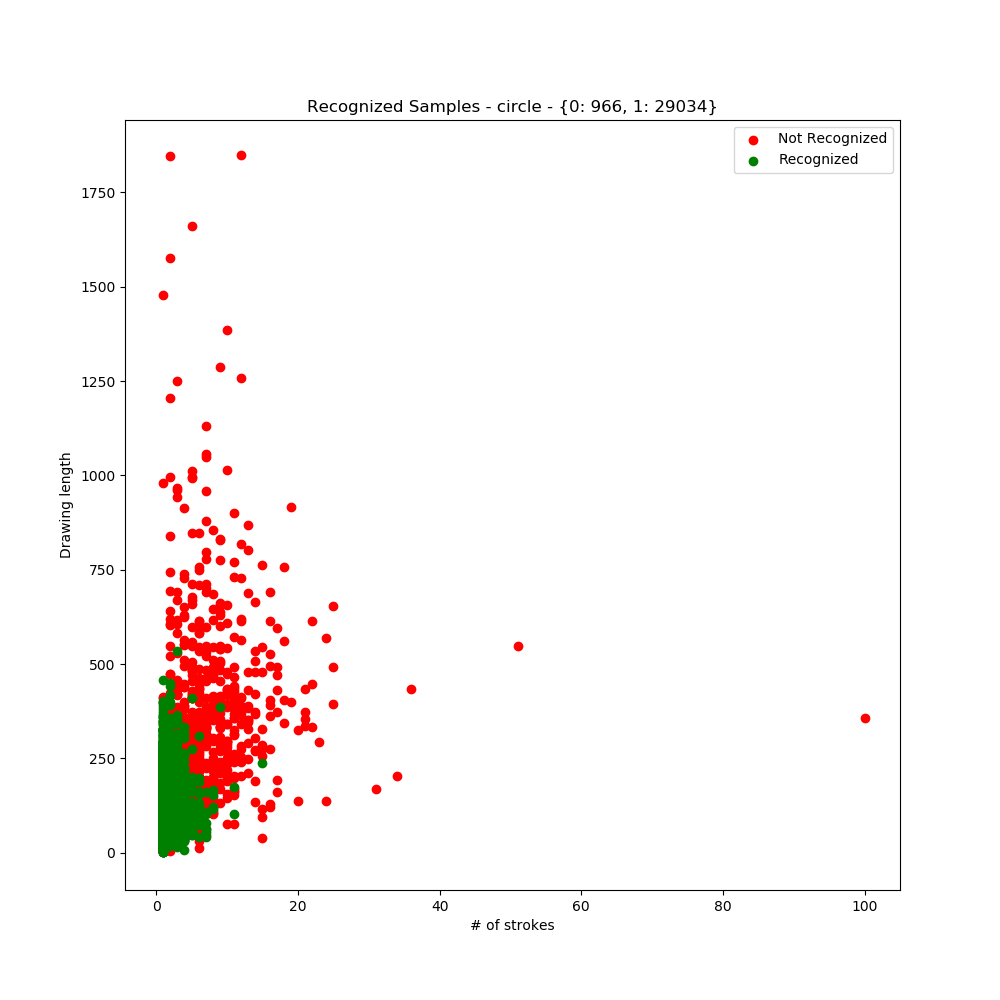
\includegraphics[scale=0.28]{images/dataset/recog_circle.png}
    \end{subfigure}
    ~
    \begin{subfigure}{0.3\textwidth}
        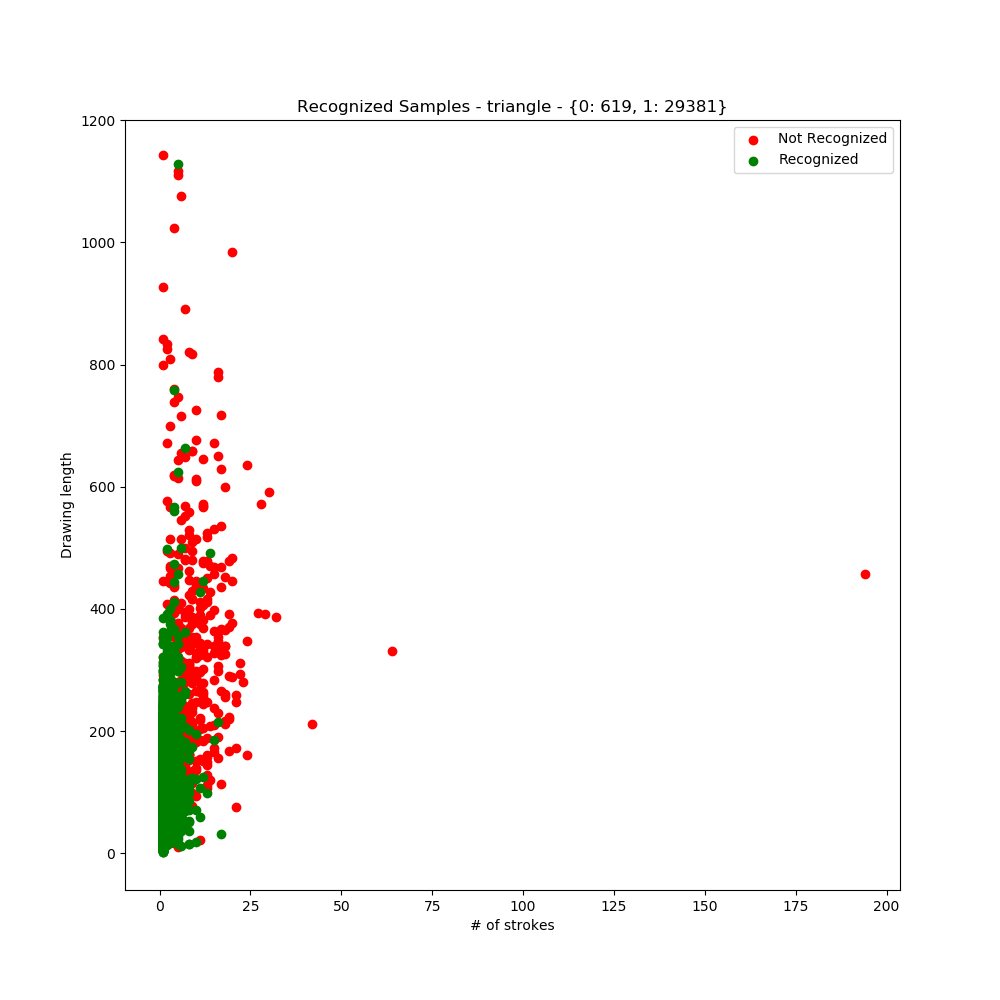
\includegraphics[scale=0.28]{images/dataset/recog_triangle.png}
    \end{subfigure}
    ~
    \begin{subfigure}{0.3\textwidth}
        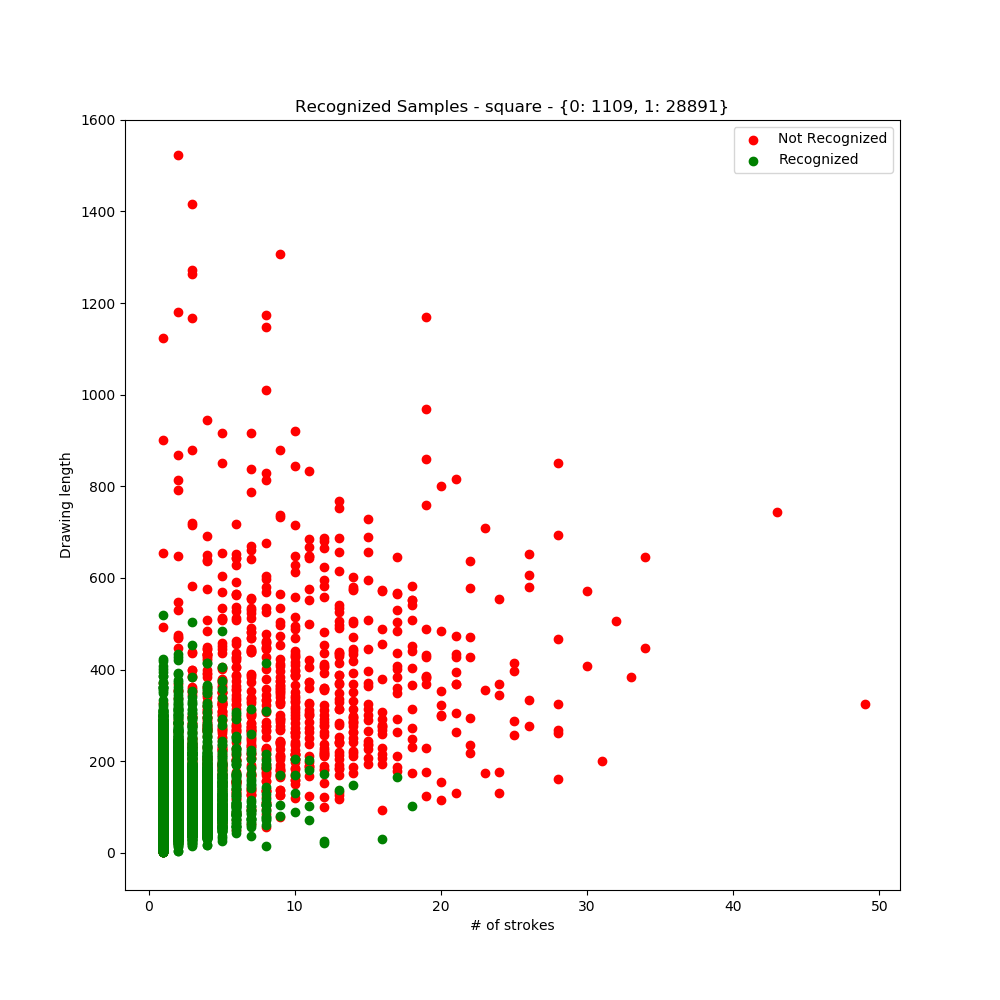
\includegraphics[scale=0.28]{images/dataset/recog_square.png}
    \end{subfigure}
    ~
    \begin{subfigure}{0.3\textwidth}
        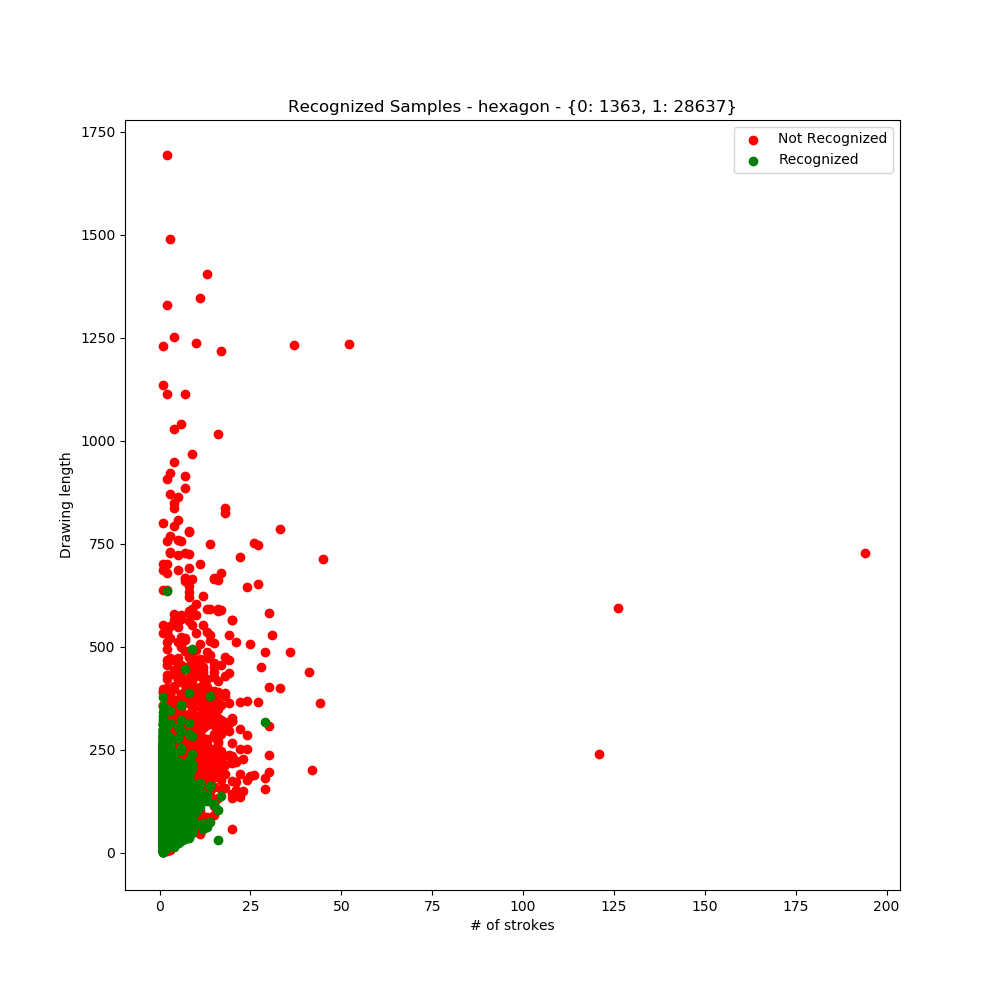
\includegraphics[scale=0.28]{images/dataset/recog_hexagon.png}
    \end{subfigure}
    ~
    \begin{subfigure}{0.3\textwidth}
        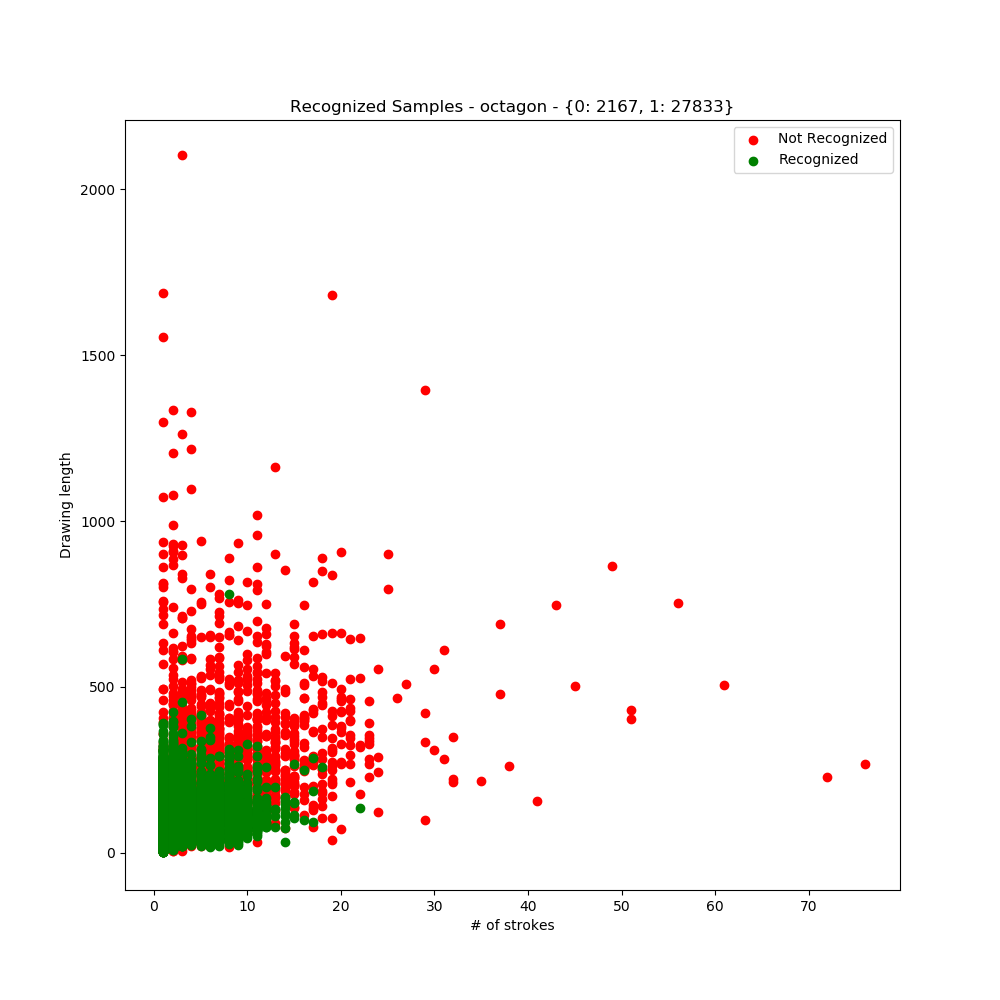
\includegraphics[scale=0.28]{images/dataset/recog_octagon.png}
    \end{subfigure}

    \caption{The distribution of the strokes in \textit{QuickDraw!} for the recognized shapes, for each category.}
    \label{fig:recognition}
% \end{figure}
\end{sidewaysfigure}

\begin{sidewaysfigure}[!htbp]
    \centering
    \begin{subfigure}{0.3\textwidth}
        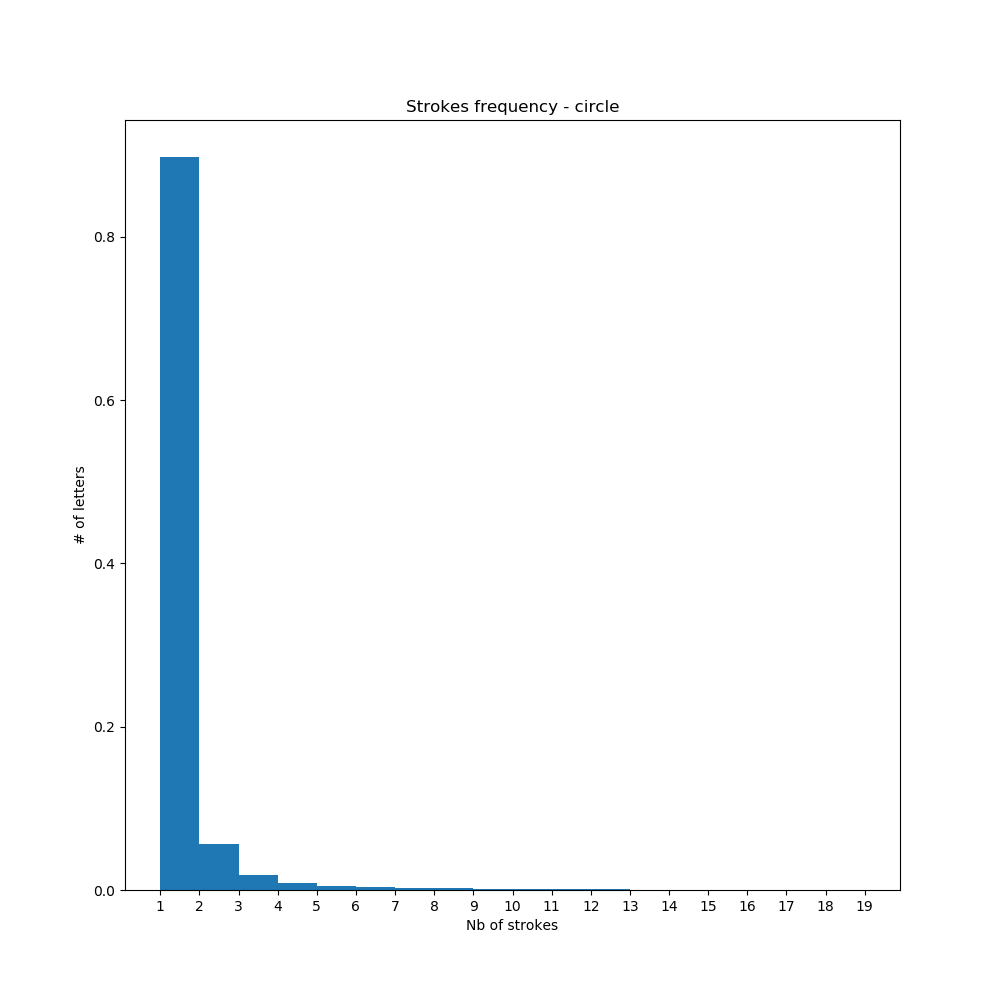
\includegraphics[scale=0.28]{images/dataset/strokes_frequency_circle.png}
    \end{subfigure}
    ~
    \begin{subfigure}{0.3\textwidth}
        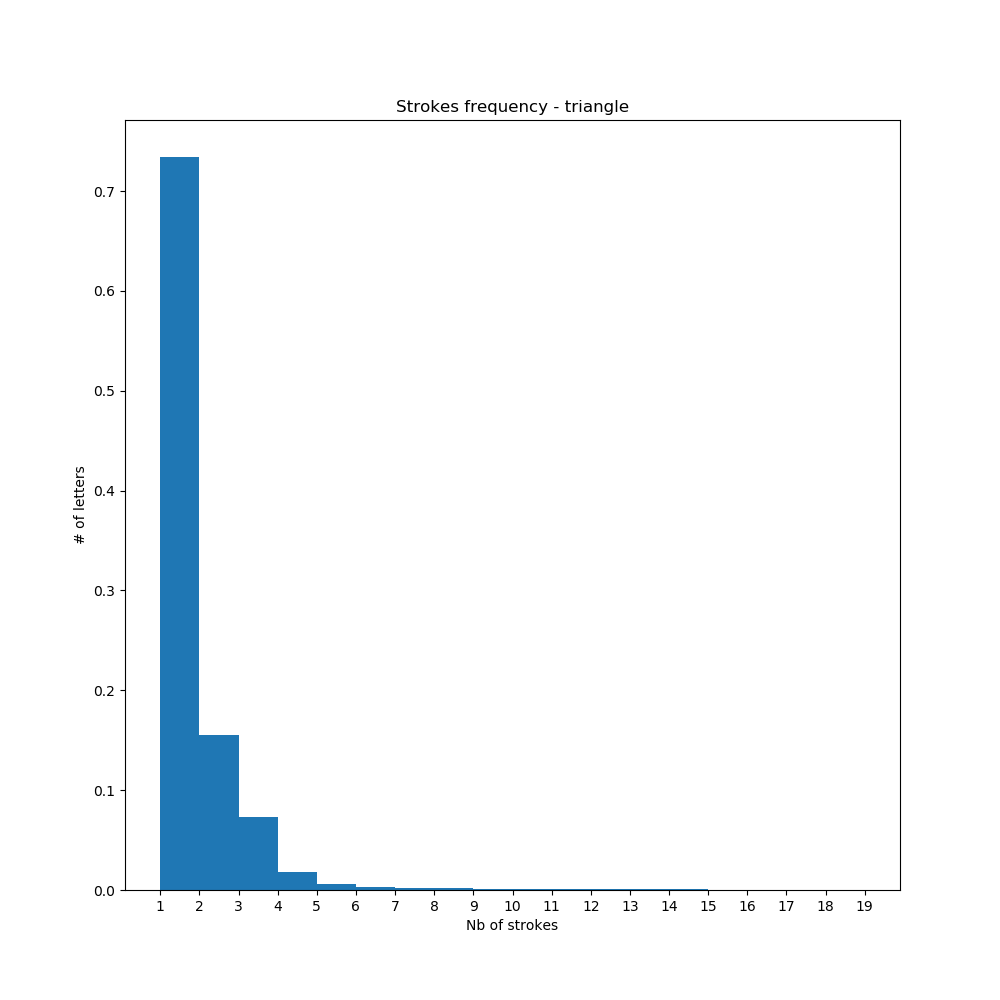
\includegraphics[scale=0.28]{images/dataset/strokes_frequency_triangle.png}
    \end{subfigure}
    ~
    \begin{subfigure}{0.3\textwidth}
        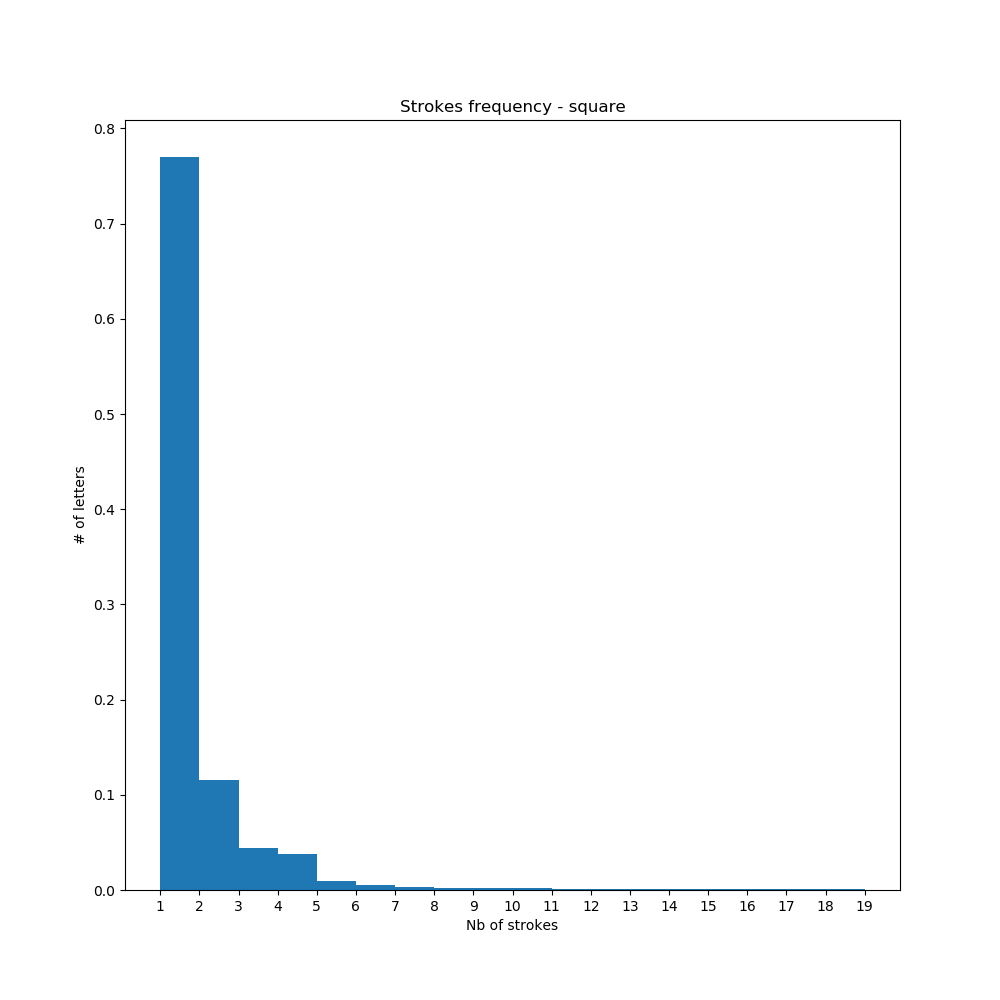
\includegraphics[scale=0.28]{images/dataset/strokes_frequency_square.png}
    \end{subfigure}
    ~
    \begin{subfigure}{0.3\textwidth}
        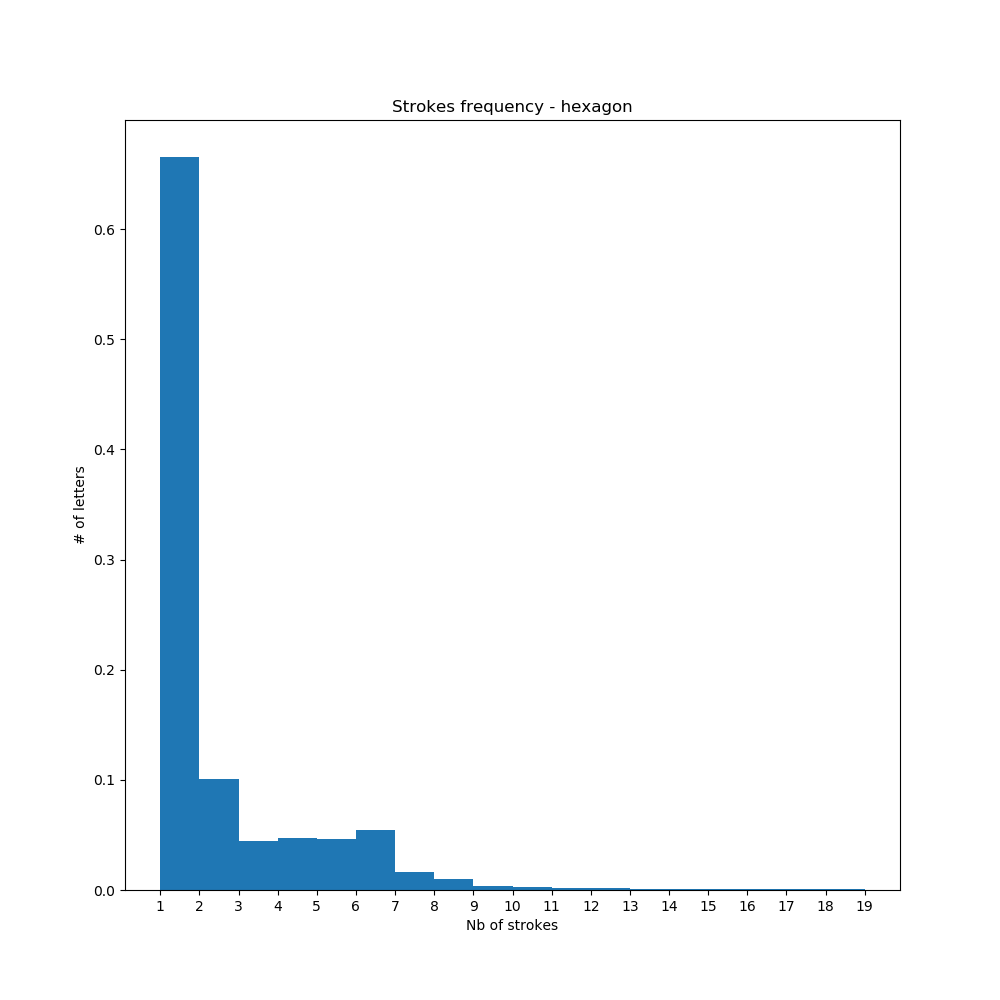
\includegraphics[scale=0.28]{images/dataset/strokes_frequency_hexagon.png}
    \end{subfigure}
    ~
    \begin{subfigure}{0.3\textwidth}
        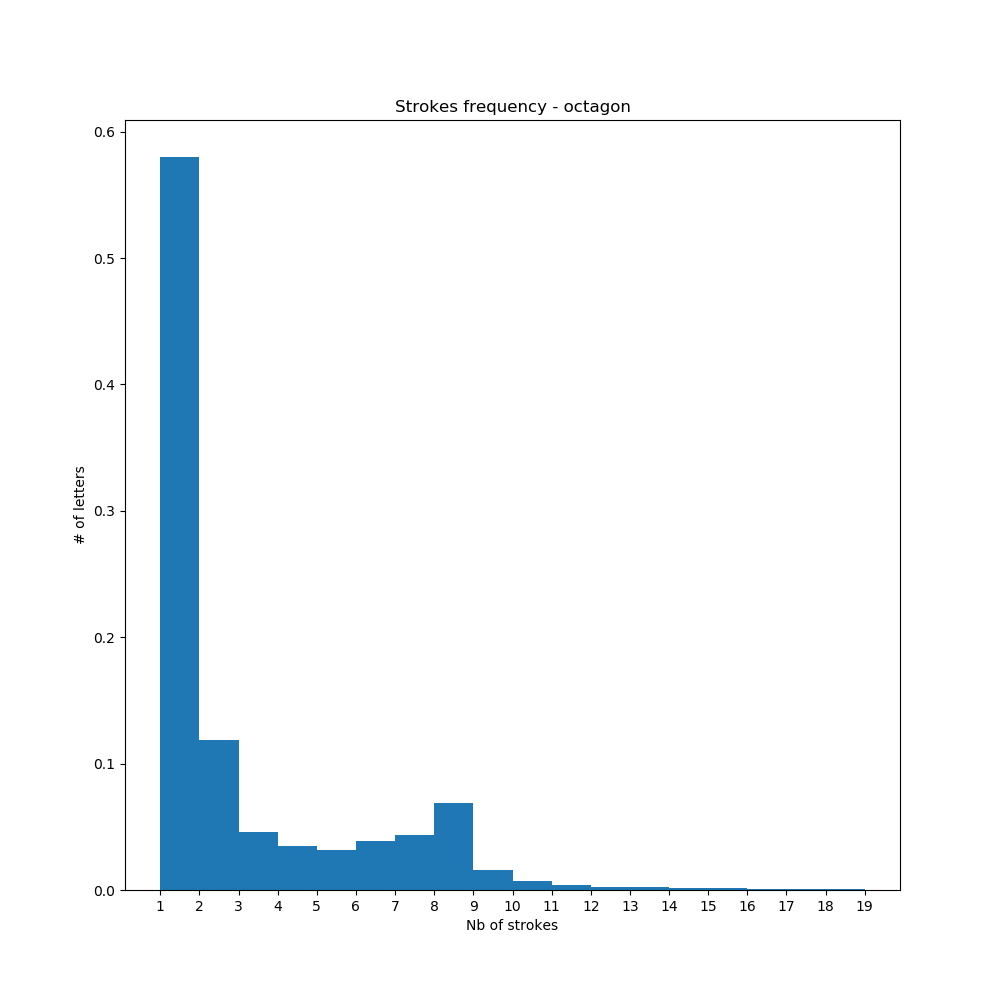
\includegraphics[scale=0.28]{images/dataset/strokes_frequency_octagon.png}
    \end{subfigure}

    \caption{The recognized VS non-recognized drawings in \textit{QuickDraw!} in each of the selected categories.}
    \label{fig:stroke_count}
\end{sidewaysfigure}

\begin{sidewaysfigure}[!htbp]
    \centering
    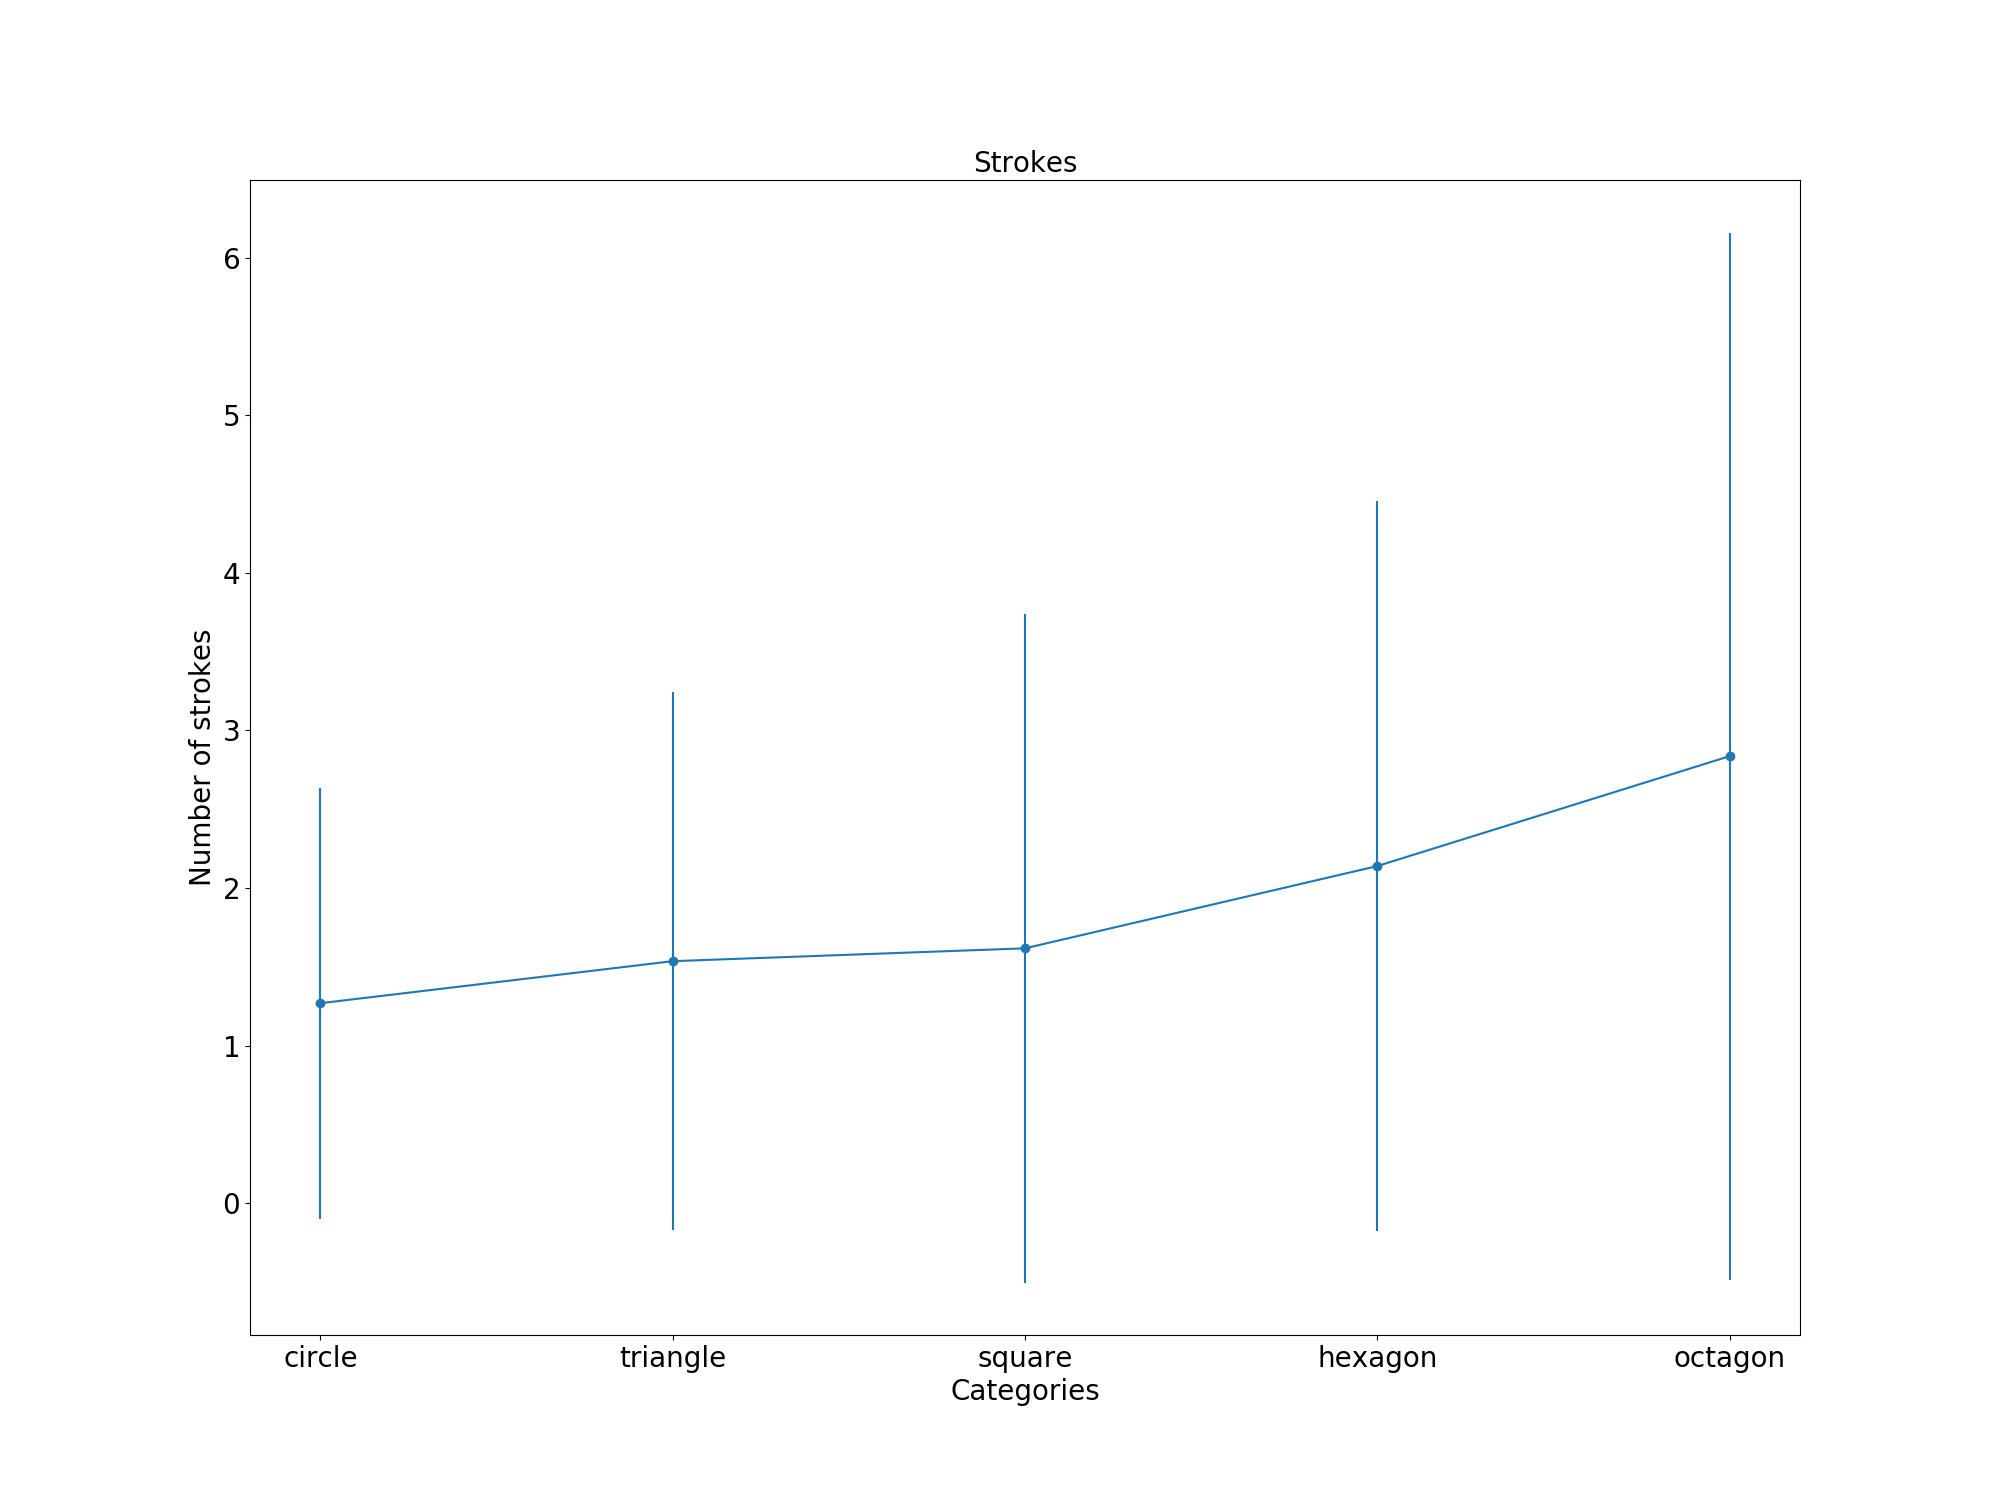
\includegraphics[scale=0.4]{images/dataset/quickdraw_strokes.png}
    \caption{QuickDraw! strokes statistics for each of the selected categories.}
    \label{fig:quickdraw_strokes}
\end{sidewaysfigure}

\begin{sidewaysfigure}[!htbp]
    \centering
    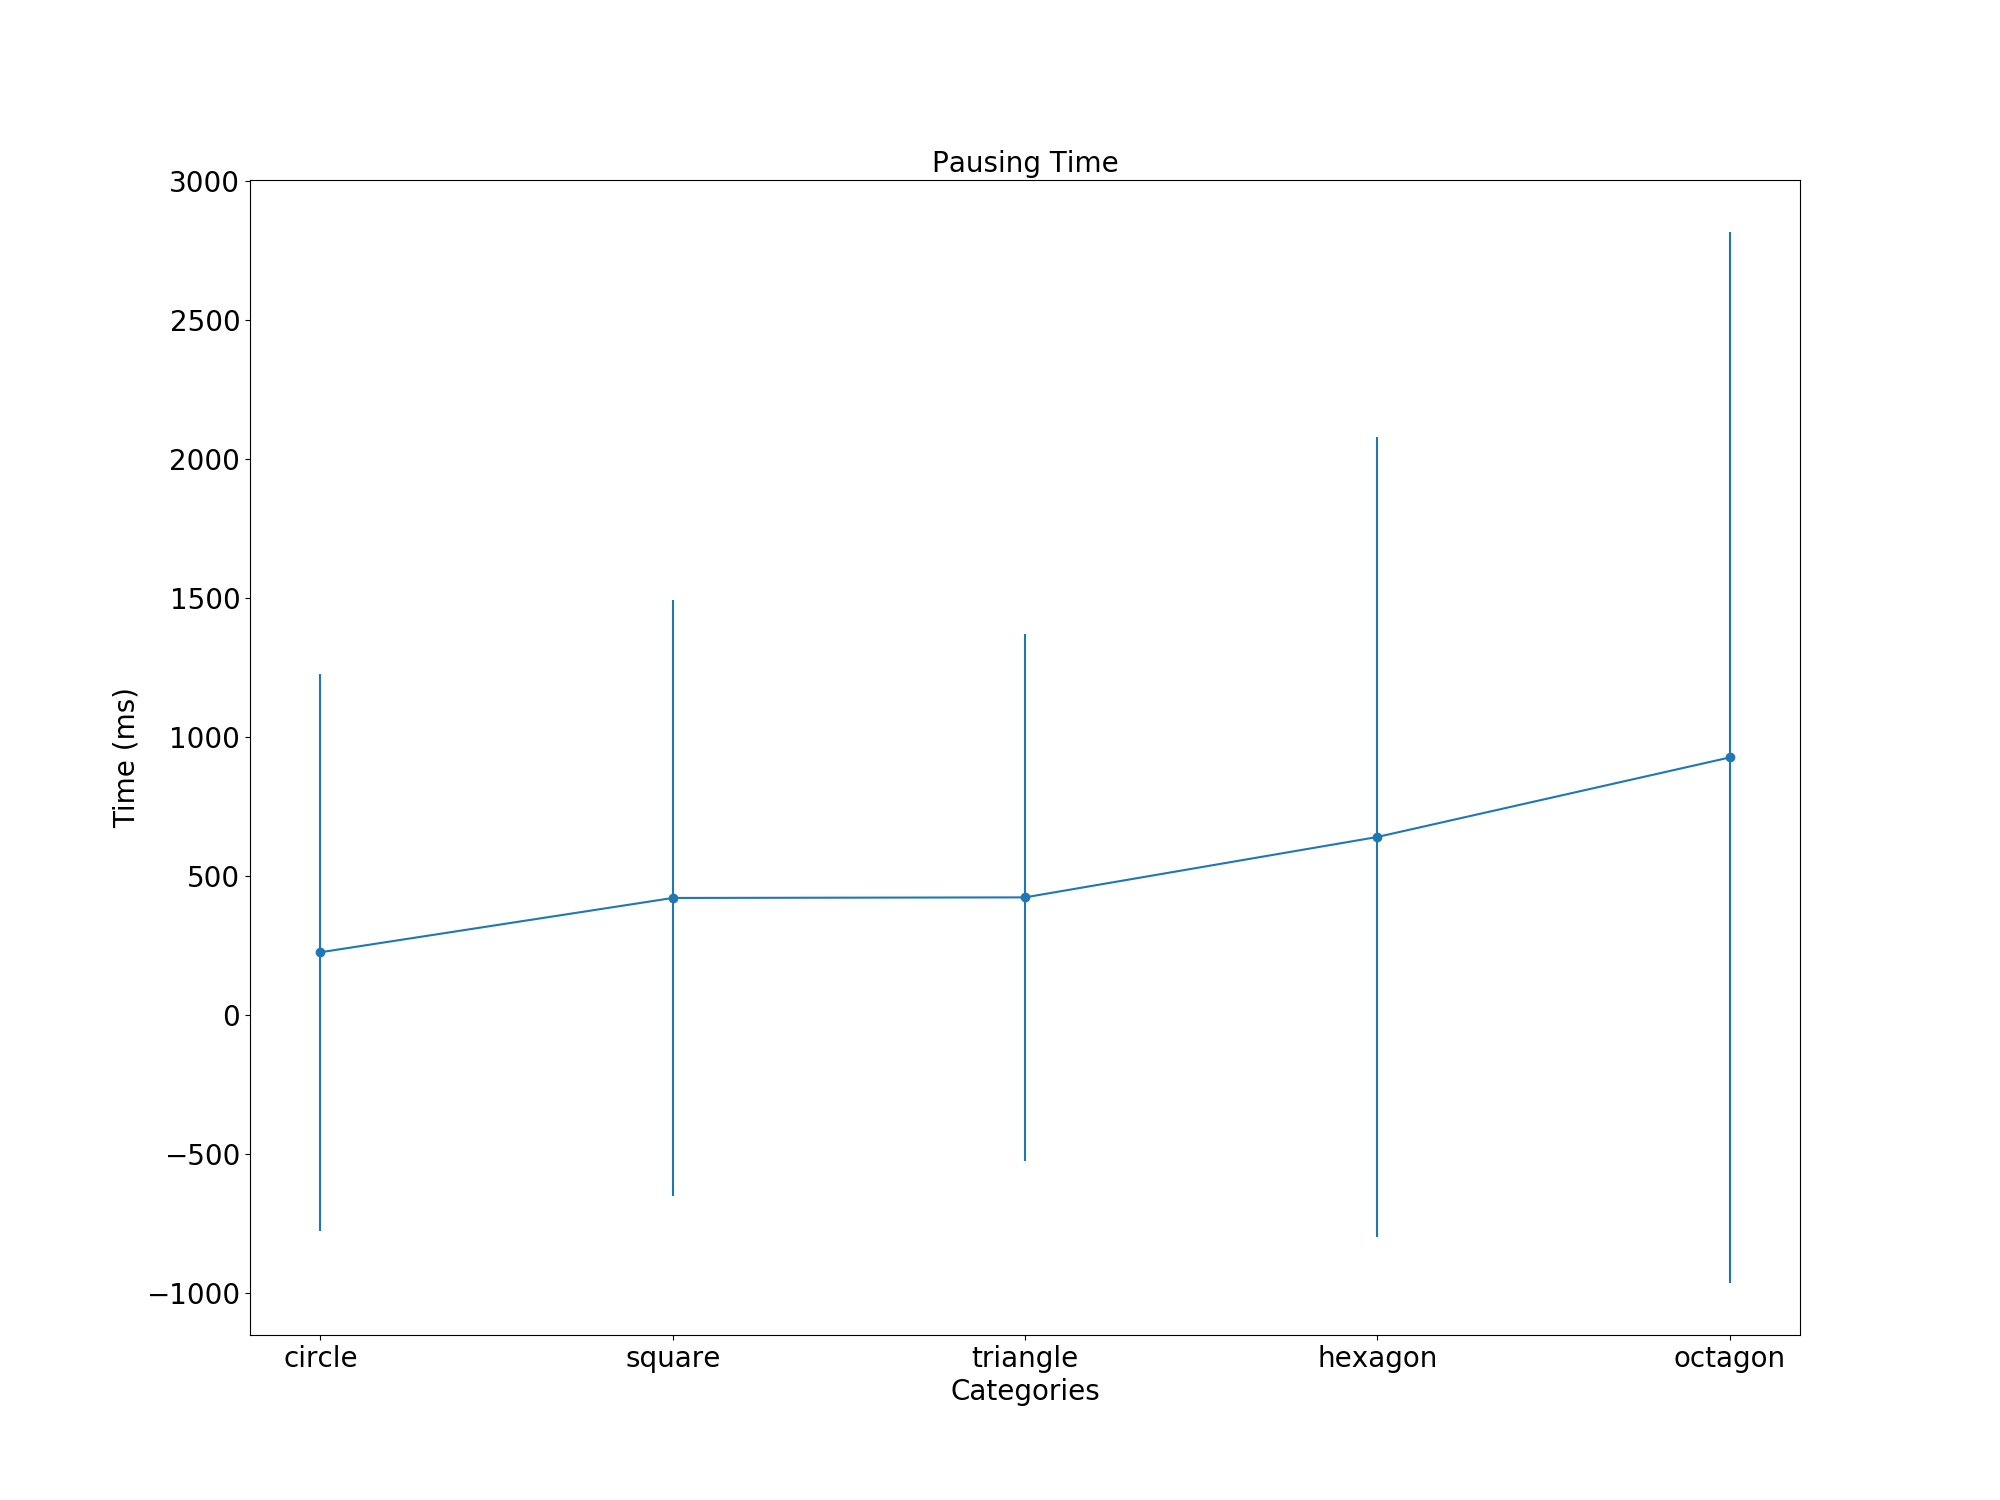
\includegraphics[scale=0.4]{images/dataset/quickdraw_pausing_time.png}
    \caption{QuickDraw! pausing time statistics for each of the selected categories.}
    \label{fig:quickdraw_pausing_time}
\end{sidewaysfigure}

\begin{sidewaysfigure}[!htbp]
    \centering
    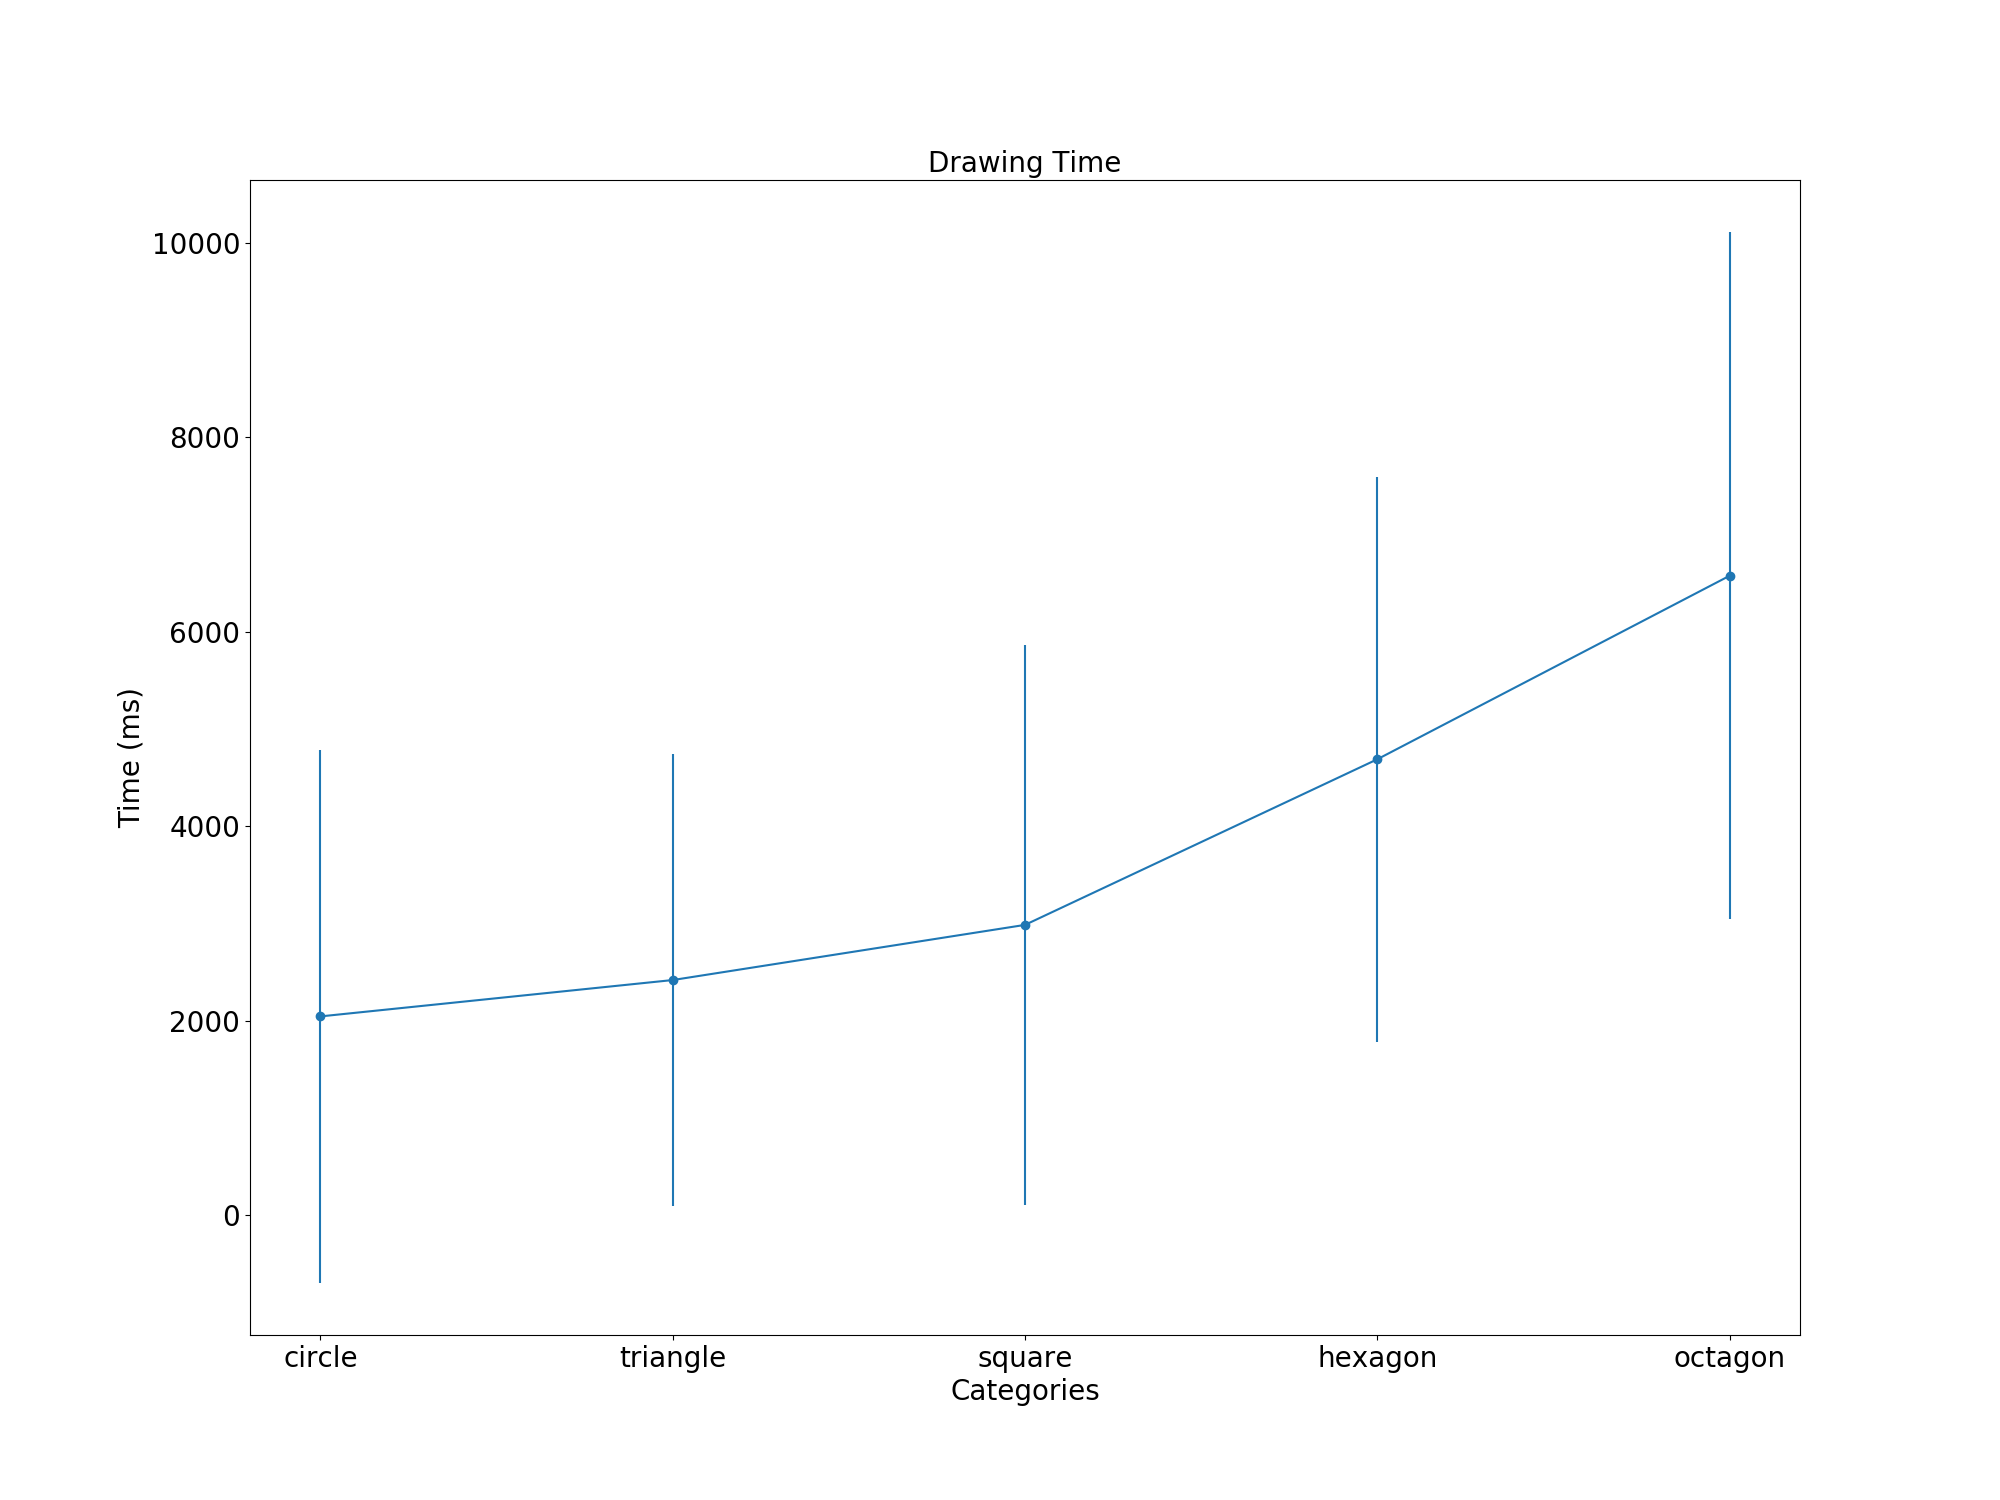
\includegraphics[scale=0.4]{images/dataset/quickdraw_drawing_time.png}
    \caption{QuickDraw! drawing time statistics for each of the selected categories.}
    \label{fig:quickdraw_drawing_time}
\end{sidewaysfigure}

\begin{sidewaysfigure}[!htbp]
    \centering
    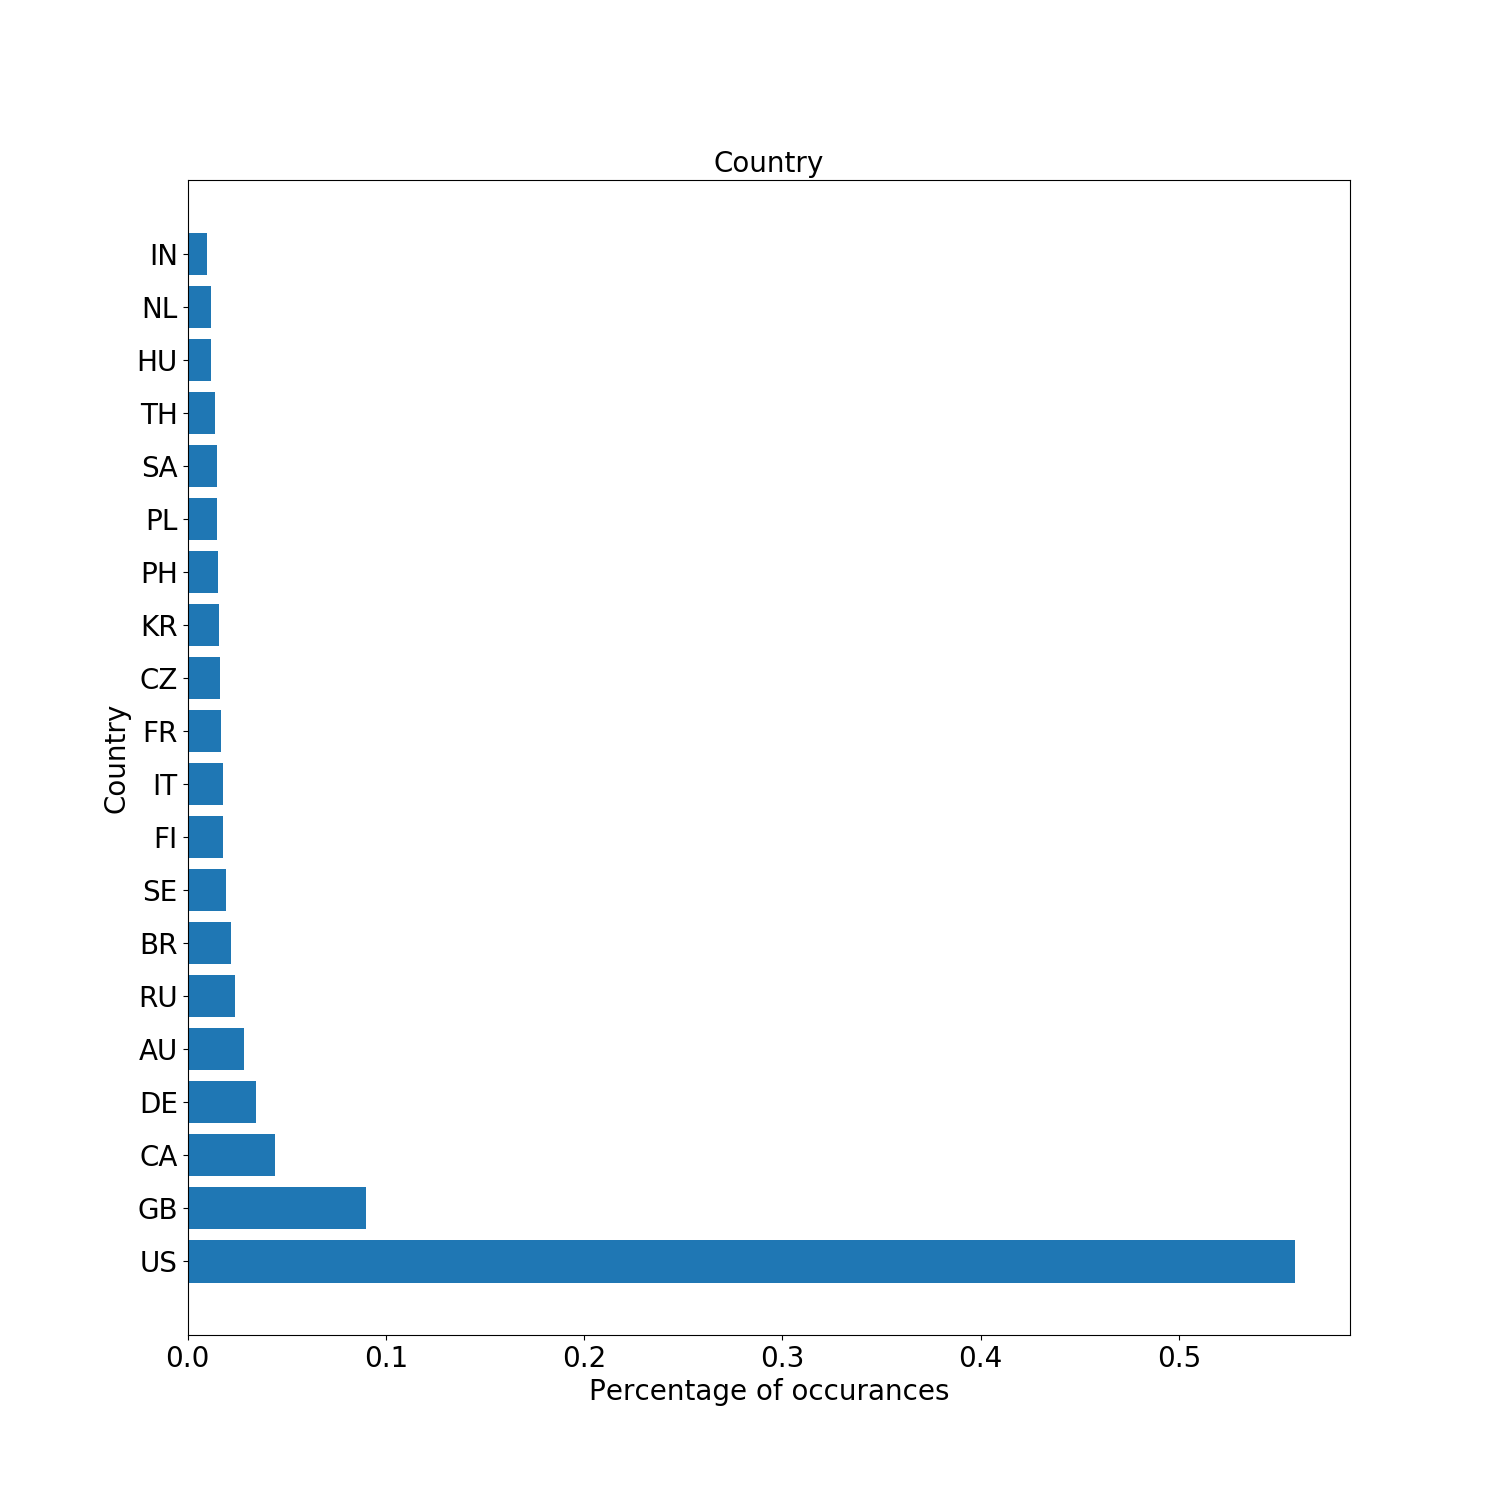
\includegraphics[scale=0.4]{images/dataset/quickdraw_countries.png}
    \caption{The most dominant countries for the players in QuickDraw! dataset. In the sample we analyzed, there is players from around 160 countries, but the majorty are from United States, followed by Great Britain.}
    \label{fig:quickdraw_countries}
\end{sidewaysfigure}

% A standard scaling process is applied on the X and Y traces, and then the feature extraction step is applied (discussed in detail in section \ref{sec:data_representation}).


\section{Data representation}\label{sec:data_representation}
  \textbf{This section should be more general, discussing both pre-processing and represenation in the same time. Otherwise, we can discuss only the representation, and move the pre-processing steps to the appendix (which makes sense). Also, there is the pre-processing part Gerard performed on QuickDraw, which should be discussed.}

  The choices of data representation is a key factor in the success or failure of the machine learning based approaches. This choice, however, is also entangled with the task to be done (in this case, the study of styles).

  A good representation tries to:
  \setlist{nolistsep}
  \begin{itemize}[noitemsep]
      \item Maximize the density of $data/patterns$ ratio: machine learning algorithms are statistical algorithms. It performs better when we have more examples for the patterns we want to learn (e.g., in case of cat/dog image recognition, having more example images for these two categories will always lead to a better performance).
      Another way is to reduce the number of irrelevant/unnecessary patterns to be learned from the data. This is the task of \textit{feature selection}, which is a fundamental step in machine learning. The target is to increase the amount of signal-to-noise ratio in the data.
      All-in-all, the objective is to increase the ratio of $data/patterns$, either by adding more data (if it is possible, or by using synthesis data using methods like \textit{Generative Adversarial Networks} \citep{goodfellow2014generative}), or removing irrelevant patterns.
      \item Simplify the learning procedure (differentiability/richness of distributions): while working with deep neural networks provide us with a lot of power in modeling a large variety of task, it also imposes some constraints.
      For example, the whole learning pipeline must be differentiable (this is a limitation imposed by the optimization methods, which will be discussed later). There are a lot of already available \textit{off-the-shelf} functions that can be used, but care must be in the design of the experiment, to make it fit with these functions.
      Sometimes however, these functions are not enough to model the task properly. Thus, there is a need to adapt new tools to fit within the neural networks paradigm. This including finding a proper way to differentiate them, or, if not possible, to move around the non-differentiability problem (usually by finding a surrogate function to optimize), which is not always a straightforward task for deep learning practitioners.
      \item Keep enough patterns to perform the intended study: it is quite tempting to focus on the scores of the machine learning algorithm, while forgetting about the original task. In our case, machine learning is a tool to help us perform our analysis, but not the final objective. For example, a low-level quantization of the X and Y traces of the pen will remove a lot of patterns, and will make it easier for the algorithm to learn the data distribution. But it will also remove essential information about the styles in this case.
  \end{itemize}

  \par In the following subsections, we will discuss two different data representation choices (continous versus discrete representation, and the features used), and the implications of each of them on the machine learning , and the study of the styles.

  \subsection{Continuous or Discrete representation?}

    \par The X, Y and pressure of handwriting tracings are always recorded as continuous distribution, while the pen state is discrete (categorical). Thus, it probably makes sense to model the data in their native form. In the neural network design, a typical design choice will be to use a linear activation function as output function, and the \textit{Minimum Square Error} (MSE) as loss function. Unfortunately, it is not that straightforward.

    \paragraph{Continuous Data Representation}
      \par To understand the problem, we first need to consider how a simple feed-forward neural network works, figure \ref{fig:mlp_simple}. The input is $x$, the output of the network is $a$, and we want to predict $y$. The neural network tries to project $x$ to a new space $z_{21}$ through a series of continuous folding of space. Then, the rule of the last activation layer is to model $P(y|z_{21})$.

      \begin{figure}[!htbp]
          \centering
          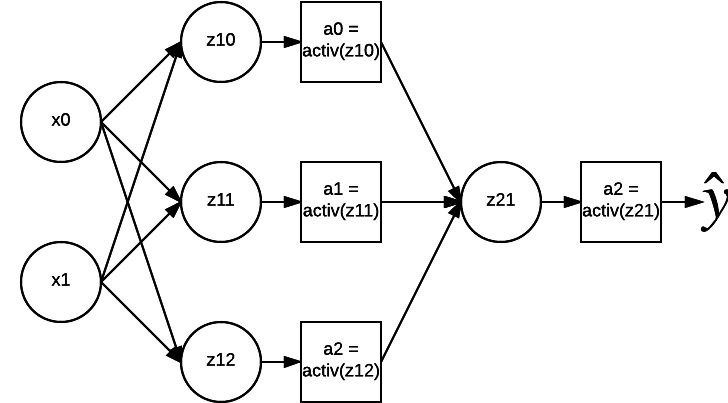
\includegraphics[scale=0.8]{images/sota/Multi-layer-perceptron2.png}
          \caption{Example of a single-hidden layer neural network. The circle units is the sum of the weighted neurons connected to this unit, and the square units is the application of the activation function on that sum.}% \textbf{MAKE A BETTER DIAGRAM}}
          \label{fig:mlp_simple}
      \end{figure}

      \par Although a linear activation is very simple, $y=z_{21}$, it is also shown to have limitations. In \citep{bishop1994mixture}, a simple example is shown (see figure \ref{fig:linear_activation_issue}). If each input $x$ gets a unique output $y$ (one-to-one mapping), then linear activation performs well (figure \ref{fig:linear_activation_issue}, left). But if the input can have multiple possible outputs (one-to-many), the model learns to average over these outputs (figure \ref{fig:linear_activation_issue}, right). The author concludes that a simple linear activation function is not powerful enough to represent a complex/rich distributions. He then proposed the use of a \textit{Gaussian Mixture Model}~\citep{Murphy:2012:MLP:2380985} (GMM) as the final activation of the neural network, which is powerful enough to enable modeling complex continuous distributions, and avoids the problems of a simple linear activation function. This combination of neural network and GMM is called \textit{Mixture Density Network} (MDN). The loss function in this case is changed from the MSE to the a posterior log-likelihood of the GMM. The neural network output in this case is not the required prediction directly, but the parameters of the GMM (means, variances, weights, correlations). The required prediction is then sampled from this parameterized GMM.

      \begin{figure}[!htbp]
          \centering
          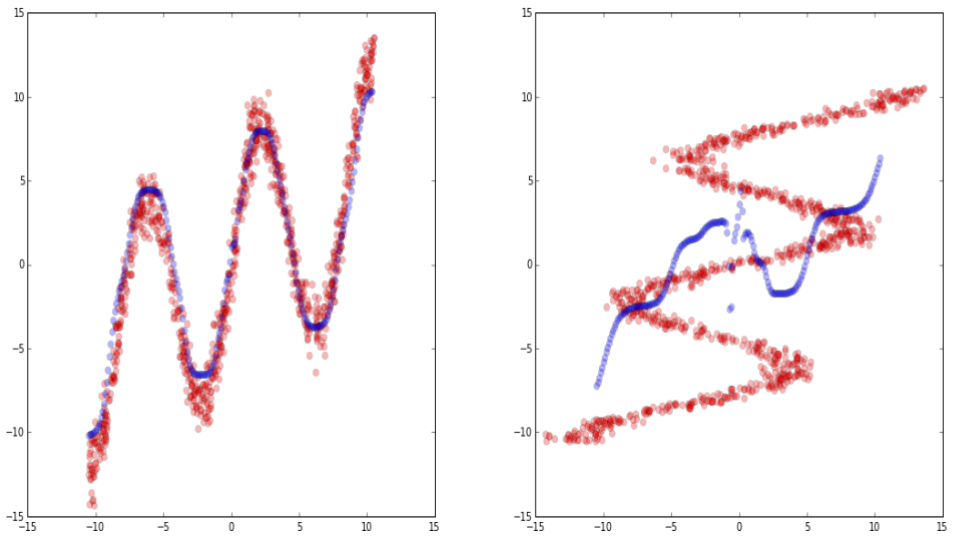
\includegraphics[scale=0.3]{images/sota/linear_activation_problem.png}
          \caption{The performance of the simple linear activation function on two setups. Left: in case of one-to-one mapping between the input and the output, it performs well. Right: In case of one-to-many mapping, the function starts to average over the seen observations, leading to undesirable behaviour. Source of this image is \citep{ha2015mdntf}.}
          \label{fig:linear_activation_issue}
      \end{figure}

      \par The work done in \citet{graves2013generating} demonstrated a system which generates impressive results on handwriting demonstration. He used an adaptation of the MDN for temporal data. Other applications for MDN can also be found in speech synthesis \citep{zen2014deep,wang2016gating,Wang2017AnAR}. While there is no question about the power the MDN approach provides, it was reported in \citep{graves2013generating} that training model kept collapsing (the explosion of gradients, the loss going to $inf$ or $NaN$), thus requiring tweaks and tricks in order to train properly. This is in-line with the experiments I performed with MDN, leading to similar conclusions.
      % \par The work done by \citep{graves2013generating} demonstrated a system which generates impressive handwriting results. In his approach, instead of using a linear activation at the end, he used a \textit{Gaussian Mixture Model}\citep{Murphy:2012:MLP:2380985}, GMM , eand changed the objective function from mse to the log-likelihood of the GMM. This idea of using GMM is called \textit{Mixture Density Networks}\citep{bishop1994mixture}, MDN. While this worked brilliantly, the author reported that training model kept collapsing (the explosion of gradients, the loss going to $inf$ or $NaN$).
      % \subsection{Discrete data representation}
    \paragraph{Discrete Data Representation}
      \par Discrete representation of originally continuous data requires transforming the data via feature engineering and/or quantization step on the raw data. While it is guaranteed there will be some information loss in the discrete data, discretization provide a lot of robustness to noise (this is why it is used in digital communication for example), and flexibility (many tools based on information theory do exist to handle digital data). Plus, a categorical distribution does not make assumption of the shape of the data distribution, unlike continuous distributions. The use of discrete distribution and how to infer from a discrete distribution will be covered later in section \ref{sec:gbem_background}.

      \par The challenge in this case is to choose a good quantization technique, that preserve the relevant information in the original signal one one side, and while keeping the dimensionality of the problem to a tractable level. For example, in case of speech synthesis, the authors in \citep{oord2016pixel,oord2016wavenet} showed that applying the $\mu$-law to the raw speech signal, and then quantize it (thus, the quantization is not linear), revealed a superb sound quality. This is better than performing naive linear quantization on the data, and saves a lot of memory as well: with non-linear quantization, they only need 256 levels. To get a similar behavior with linear quantization, around 65K quantization levels or required.

  \subsection{Feature engineering: Direction and Speed}
    \par As argued in the previous section, we choose discrete representation for our data. A requirement for a good quantization scheme should keep the important information in the original signal\sidenote{In some applications, like in digital communications for example, the quantization (or digitization process) has other rules, like compressing the signal, increasing the signal-to-noise ratio, and increase the robustness of the signal. This is outside the scope of our work however.}

    \par In case of \textit{IRONOFF}, the letters tracings has been cleaned by removing points related to false starts or corrections as well extra strokes. Tracings were re-sampled with $10ms$ time interval, and the ones with length exceeding 1 second has been removed, as well as tracings more than 100 time steps. This is because they are quite rare, thus, their existence would significantly degrade the performance of our model.

    \par For \textit{QuickDraw!}, the re-sampling interval is $20ms$, and consider tracings that are less than 200 time steps. This is because the tracings tend to be longer than in \textit{IRONOFF}. This start to became more clearer when the task gets more complex (the octagon being the most complex one).

    \par We represent each letter tracing by two features: directions and speed. Each feature is quantized into 16 levels and represented as a one-hot encoded vector.

    \par Freeman codes \citep{freeman1961encoding} is used in order to encode the direction feature. It belongs to a family of compression algorithms called \textit{Chain Codes}. This set of algorithms proved to be useful to encode an image with connected components. They can transform a sparse matrix to just a small fraction of the size of the image, in the form of a sequence of codes. Thus, they are being used as compression algorithms as well.

    \par Freeman codes can N-directional codes (where N are the directions), depending on the needed resolution. It is quite simple as it encodes each direction with a unique number from 0 to N-1. A direction is defined as the directed vector connecting two neighbouring pixels on the contour of a connected component in the image.

    \par We compute the change of directions between three consecutive points. Then, we map this change to its corresponding freeman code number, as shown in figure \ref{fig:freeman_dir}. Last, we transform the direction number into one-hot encoding scheme, and use this as input to our network. We also quantize the speed of each displacement.

    \begin{figure}[htbp!]
    \centering
    \includegraphics[scale=0.7]{images/dataset/Freeman_dir.png}
    \caption{Example for freeman code representation for 8 directions. Each direction is given a unique number.}
    \label{fig:freeman_dir}
    \end{figure}

\section{Summary}
  \par In this chapter, we explored two datasets: Cursive Handwriting dataset, \textit{IRONOFF} and sketch drawing dataset \textit{QuickDraw!}. Each of these datasets contains several tasks/categories (the letters/digits in case of \textit{IRONOFF}, and the shapes in case of \textit{QuickDraw!}), and we can explore the styles around each of those tasks. We explored basic information about each task (number of strokes, drawing time, and the pausing time).

  \par We motivate the use of these datasets because we can see that there is a variance in these information of each task, suggesting different styles for each task. This variance differs a lot depending on the complexity of tasks: in \textit{IRONOFF} for example, letter \textit{c} seems to be the simplist task, thus, the variance in it is relatively not that large. This variance increases as the task get more complex (letter \textit{E} for example). In \textit{QuickDraw!} dataset, a similar trend can be observed (the \textit{circle} being the simplest task, and the \textit{octagon} being the most complex one).

  \par Last, we argue that although that \textit{QuickDraw!} has simpler tasks than \textit{IRONOFF}, it is actually more complicated. We hypothize that this is due to the fact that there is a huge variety in the players (many different countries, compared to mosty \textit{French} people in \textit{IRONOFF}). The players use mostly the mouse in order to draw\sidenote{The players did not receive any special training on drawing with the mouse beforehand.}, which leads to behaviors usually unobserved with hand drawing/writing. Also, in such environment, it is expected that the human curioisty will prevail, and people will try to draw complex shapes, outside the limit of the required task, in order to see if the neural network classifier will recongize it correctly or not.

  \par We will consider that there are two heirarichty of tasks in \textit{IRONOFF}: the first is uppercase, lowercase letters, and digits. The second is the individual letters and digits. When we perform transfer learning, we will do it on the tasks of the first heirarichy only (for computational reasons).

  \par We will use \textit{QuickDraw!} side-by-side to \textit{IRONOFF} in our last part of our work in order to validate our approach and conclusions, but the first two parts will be done on \textit{IRONOFF} only.
% \par \OSM{Compare the reconstruction error between naive digitization of the pixels and the use of freeman and the speed, on the same number of bins -> 32 total}

% \par \OSM{Should we say that speed feature is important? I really don't think so, since we don't have any support for this argument.}

% \theendnotes
% \setcounter{endnote}{0}

\part{Experiments}
% \chapter{Generative models, benchmarks and evaluation metrics}
\chapter{Generation, benchmarks and evaluation}\label{ch:GBEM}

\minitoc% Creating an actual minitoc

\par Since styles are ill-defined, they can not be evaluated explicitly (we can not quantify them in advance). Thus, we need a proxy method in order to implicitly evaluate them. We can do this by using them in order to generate behaviors (i.e., synthesis handwriting traces), and evaluate the quality of those behaviors relative to the target behaviors (i.e., the original letters traces). In other words, to study styles, we would like to use reconstruct the target behaviors using generative models, and given the task and the styles to perform the behavior. We discuss the recent advances in neural generative models: how are they trained? how do we infer from them?. Then we look at paradigm for reconstruct target behaviors, with focus on the usage of neural networks.

\par After we generate the behaviors, we need to evaluate them in a manner that evaluates the styles. This is still an open research question, and a complicated one as well. It also goes hand-in-hand with the choices made in generative models. We discuss the used evaluation metrics across different domains (e.g., text, speech and handwriting evaluation). We also discuss the difficulties associated with finding the suitable evaluation metric.

\par I then present the experiments done in order generate letter and ground our proposed evaluation metrics. I will explain our choices for the model design, the inference methods, and our approach to ground the metrics.

% \par This chapter sets the foundation for the PhD.

\begin{mdframed}[backgroundcolor=blue!20]
    \begin{center}
        Questions addressed in this chapter
    \end{center}

    \begin{itemize}
        \item How to generate handwritten letters using deep learning framework?
        \item How to evaluate the generated traces?
        \item What benchmarks are suitable to compare to?
    \end{itemize}
\end{mdframed}

\clearpage

\section{Background}\label{sec:gbem_background}
\par We start by introducing the different basis in the literature for our work. Most of this work uses deep learning and generative models. How and why deep learning emerged in the last few years is quite important to keep in mind, since it is the starting point for any successful usage of deep learning. We then explore a particular aspect of deep learning: generative models. In particular, we focus on the domain of sequential data, where the problem gets more challenging. A direct consequence for using generative models is the challenge of evaluating what is generated. Generation, after all, is an artistic aspect, unlike well defined machines learning tasks like regression and classification. We try to make sense of what exists in the literature, and try to deduce what would be a good criteria for new evaluation metrics for a generative task.
% \subsection{Deep Learning: quick overview}
% \textbf{\textsc{this part will be modified. focus only on RNN, leave generative models to the next section}}
% \setlist{nolistsep}\begin{itemize}[noitemsep]
%     \item Talk about deep learning and its current uses in general
%     \item
% \end{itemize}

\par Deep learning is a subset of machine learning~\citep{lecun2015deep,Goodfellow-et-al-2016}, mainly applicable on neural networks. These set of techniques perform remarkably well nowadays on a wide range of tasks and benchmarks (for example, in image recognition~\citep{krizhevsky2012imagenet,simonyan2014very,he2016deep}, speech synthesis~\citep{oord2016wavenet}, image segmentation, handwriting recognition, image captioning~\citep{DBLP:journals/corr/VinyalsTBE14,karpathy2015deep}, language translation\citep{sutskever2014sequence}), even outperforming humans in some of them (GO game~\citep{silver2016mastering}).

% \GB{I would distinguish between recognition tasks (that discard irrelevant variability) and generation/prediction tasks (that have to deal with output variability)}
% \OSM{07/06: Noted. Will update it.}

% Before deep learning, in order to use machine learning algorithms were good to find patterns, given good features. This task, referred to as \textit{feature engineering}, was quite challenging in many applications (like identifying objects in images for example \textbf{PUT SOME REFERENCES HERE}), and require specific skills related to the domain of interest.

\par Before deep learning, in order to use classical machine learning algorithms, an important step was \textit{feature engineering}: extracting the relevant features from the data, in order to get the relevant information needed to perform the task. In images, techniques like \textit{Scale-invariant feature transform} (SIFT) \citep{lowe1999object}, and in speech, feature like \textit{Mel-frequency cepstrum} (MFCC) and \textit{Probabilistic  Linear  Discriminate  Analysis} (PLDA) \citep{narang2015speech}, were quite dominant at that time. There is no one solution that fits all here; it depends on the task in hand, and that required experience. Thus, feature engineering was quite challenging.

The advantage of deep learning techniques is that it overcome (to a big extent) the need for the daunting task of feature engineering. Instead, it tries to learn, from the raw data, hierarchy of features, that are optimal in order to solve the task in hand (i.e., it performs \textit{automated feature engineering}). In our work for example, we did not need to do any kind of temporal feature extraction.

\par A detailed discussion into the basics of deep learning is out of the scope of this document (and has been done properly in many books and tutorial available online). We refer you to the excellent book \citep{Goodfellow-et-al-2016} for more theoretical treatment of deep learning, and to \citep{chollet2017book,geron2017hands} for a more practical aspect.
% GB: not fan:
%\textbf{Write about the history of deep learning, and how did it become the way it is now - algorithmic\citep{srivastava2014dropout}, hardware, data, software frameworks and language... -}

\subsection{Sequential data} \label{sec:seq_data}
\par Sequential data appears in a lot of our daily life, for example: text, speech, the weather status,...etc. In a more formal manner, a sequential data example is formed of tokens, and can be represented as $x_1, x_2, ..., x_N$, where $x_n$ is one token, and $N$ is the total length of this sequential data point.

\par Let's take a more concrete example: text. We have multiple sentences in a given text. We can consider each sentence as a data point/example. If we consider an example sentence: \textit{the cat is eating the food}, and we define our tokens to be the words\footnote{There is no rule here for how we define the tokens. We can, for example, define the letters to be our tokens. In the case of text, it is a tradeoff: considering words as tokens allow the model to be more fluent, but it also means that the learning space is very large (sometimes the number of unique words to predict at each time step is in the order of tens of thousands). If we consider letters as tokens however, it make the model job more tractable (all the letters, symbols, digits, can be in the order of tens), but it leads to less quality for the model.}. In this case, $x_1=the$, $x_2=cat, \dots\ etc$.

\par What is common between all the sequential data (and what also distinguish them from non-sequential data points) is that each token is dependent on the previous token/s. In general, when we want to model sequential data, we in essence want to learn the following probability distribution:
\begin{equation}
    p(x_1, x_2, ..., x_N) = p(x_1) \times P(x_2|x_1) \times p(x_3|x_2, x_1) \times .... \times p(x_N|x_1 ... x_{N-1})
    \label{eq:rnn_obj_training_0}
\end{equation}

\par In order to model such a distribution using neural networks, we can either:
\begin{enumerate}
    \item Adding a \textit{state variable} in order to factorize the problem. In this case, we introduce an intermediate state variable, $h$, which model the dependency on the previous tokens. Our objective in this case will be
    \begin{equation}
        p(h_n) = p(h_{n-1}, x_{n})
        \label{eq:rnn_factorization}
    \end{equation}
    This can be done using \textit{Recurrent Neural Networks} (RNN), which will be explained later in detail (section \ref{sec:RNN}). In this case, the network is looping over the tokens one-by-one, updating the state variable each time.
    \item Use the whole sequential data (all its tokens) as input to the network in the same time. In this case, the network is trying to model equation \ref{eq:rnn_obj_training_0} heads-on. This approach has gained popularity recently with the work done in \citep{oord2016wavenet,gehring2017convolutional}, using convolution networks in order to model sequential data (speech for the first, language text for the second). The advantages of this approach is removing the sequential aspect of the network, and leveraging parallelism when treating the whole sequence. This results in faster training, while still achieving state-of-the art results.
\end{enumerate}

\par There is no one solution that fits all here, it simply depends on the problem and the constraints on the solution. In case of variable-length sequential data, the first approach is the one to go for. In the case of fixed-length sequential data, the second approach should be considered (easier to train the model, faster to optimize, faster to infer from).

\subsection{Recurrent Neural Networks and Sequence Modeling} \label{sec:RNN}
As mentioned briefly in the previous section (\ref{sec:seq_data}), \textit{Recurrent Neural Networks} (RNN) is a type of neural networks, that can handle sequential aspect in data. In its simplest format, it is a simple feed-forward network, applied on each token in the sequential data point, while carrying the information about the previous tokens using a latent variable $h$, commonly referred to as \textit{the hidden state variable}. This is demonstrated in figure \ref{fig:basic_rnn_model}.

\begin{figure}
    \centering
    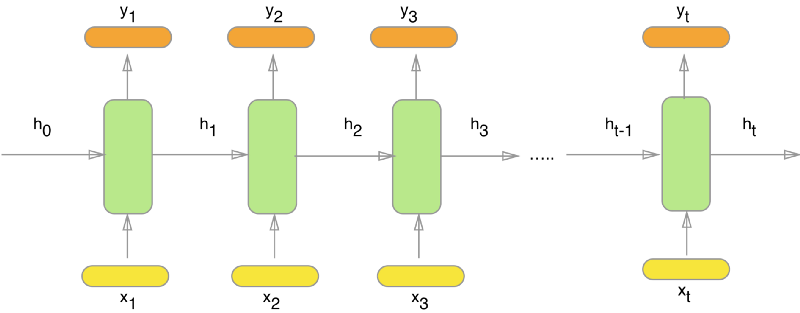
\includegraphics[width=\textwidth]{images/gbem/basic_rnn.png}
    \caption{A demonstration of how RNN works: the network is applied on each token in the input ($x_1, x_2, ..., x_t$), while update the hidden state variable every time ($h_0, h_1, ..., h_t$). The output at each step is a function of the hidden state variable (not demonstrated here). Source of the image is \citep{howrnnworks}.}
    \label{fig:basic_rnn_model}
\end{figure}

\par To describe it in a more formal manner, let's first assume the following:
\begin{itemize}
    \item The input $x$ is first processed by a set of weights, $W_{ih}$, and bias $b_{ih}$.
    \item From each step to the other, the hidden state $h$ is processed via a set weights, $W_{hh}$, and bias $b_{hh}$.
    \item Last, the output is given by processing the hidden state $h$ via another set of weights, $W_{ho}$, and bias $b_{ho}$.
\end{itemize}

\par If we assume that output activation is a simple linear layer (thus, it is a regression task), then the equations of this simple RNN are the following:
\begin{align}
    \begin{split}
    z_n = W_{ih} \cdot x_{n} + b_{ih}
    \\
    h_n = W_{hh} \cdot [h_{n-1}, z_{n}] + b_{hh}
    \\
    y_n = W_{ho} \cdot h_{n} + b_{ho}
    \label{eq:rnn_equations}
    \end{split}
\end{align}

\par Where the brackets $[\ ]$ indicate a concatenation process. In case of a simple regression task, a typical loss function is the \textit{Minimum Square Error}, which can be formulated as:
\begin{equation}
    Loss = \frac{1}{T \times N} \sum_{n}^{N} \sum_{t}^{T} \left ( y_{n, t} - \hat{y_{n, t}}\right )^2
    \label{eq:loss_fn_mse}
\end{equation}
where $T$ is the length of the sequence, and the $N$ is the number of sequential data points available, and $\hat{y_{n, t}}$ is predicted output by the model, while $\hat{y_{n, t}}$ is the ground truth output.

\par Given this formalization, the objective is to find the set of weights and biases of the network, that will minimize the chosen loss function. We will explore the optimization algorithms in section \ref{subsec:optimization}.

\subsection{Optimization Algorithms} \label{subsec:optimization}
\par One of the important factors in the recent success of deep learning is the advances in optimization algorithms. These algorithmic advances make the optimization easier, converges to a better solution, and less tweaking is required in order to achieve a good performance. All these methods are derivatives of gradient descent optimization, defined as \citep{gradientdescent}:

\begin{quote}
    Gradient descent is a first-order iterative optimization algorithm for finding the minimum of a function. To find a local minimum of a function using gradient descent, one takes steps proportional to the negative of the gradient (or approximate gradient) of the function at the current point.
\end{quote}

\par If the function to be optimized is convex \citep{convexfn} -- differentiable, and have a global optima --, then gradient descent can find this global optima. An example for the different optimization iteration can be seen in figure \ref{fig:grad_descent}.

\begin{figure}
    \centering
    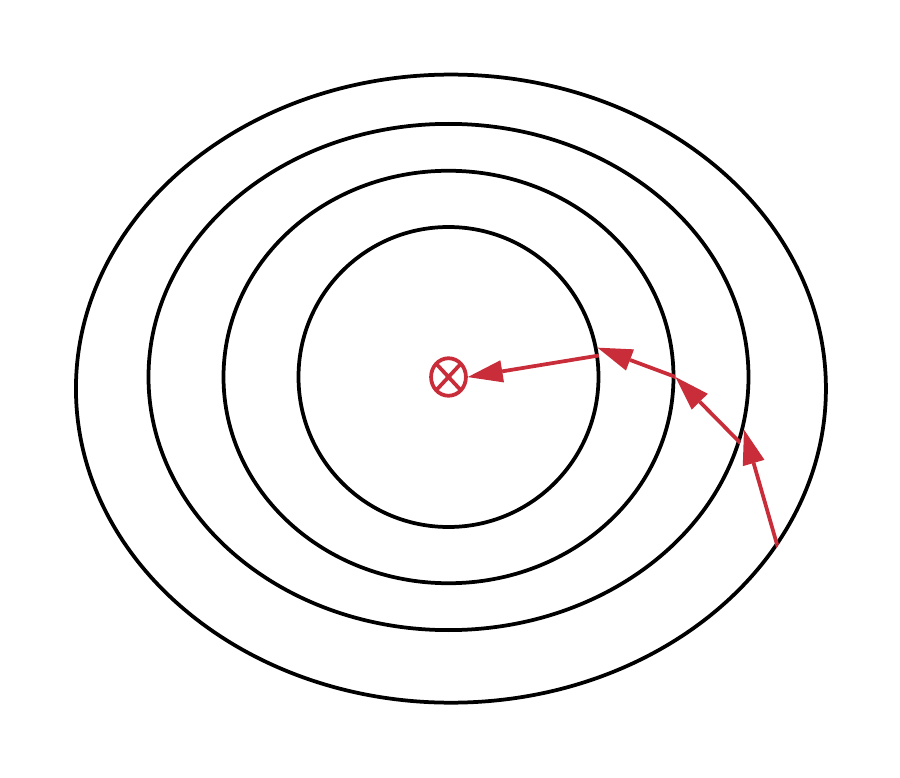
\includegraphics{images/gbem/grad_descent.png}
    \caption{A demonstration for how a gradient descent algorithm work. The optimization process progress each step towards the global optima (the indicated point in the center).}
    \label{fig:grad_descent}
\end{figure}

\par Gradient descent can be formalize by the following equation:
\begin{equation}
    % \theta_{t+1} = \theta_{t} - \alpha \times \dv{Loss(\theta_t)}{\theta_t}
    \theta_{t+1} = \theta_{t} - \alpha \times \frac{d Loss(\theta_t)}{d\theta_t}
    \label{eq:grad_descent}
\end{equation}
where $\theta$ refers to the parameters we want to optimize, $t,t+1$ refers to the current and the next iterations respectively, $\alpha$ is the learning rate (how large the step to take at each iteration), and $Loss$ is the loss/objective function we want to optimize our parameter for. Optimization by gradient descent is a \textit{batch optimization}: the loss function and its gradient is calculated all given data examples. This iterative process keeps going till we wither do not observe a tangible change in the performance of the parameters, or we exhaust our computational budget. An illustration for this process can be seen in figure \ref{fig:grad_descent_inuitive}.

\begin{figure}
    \centering
    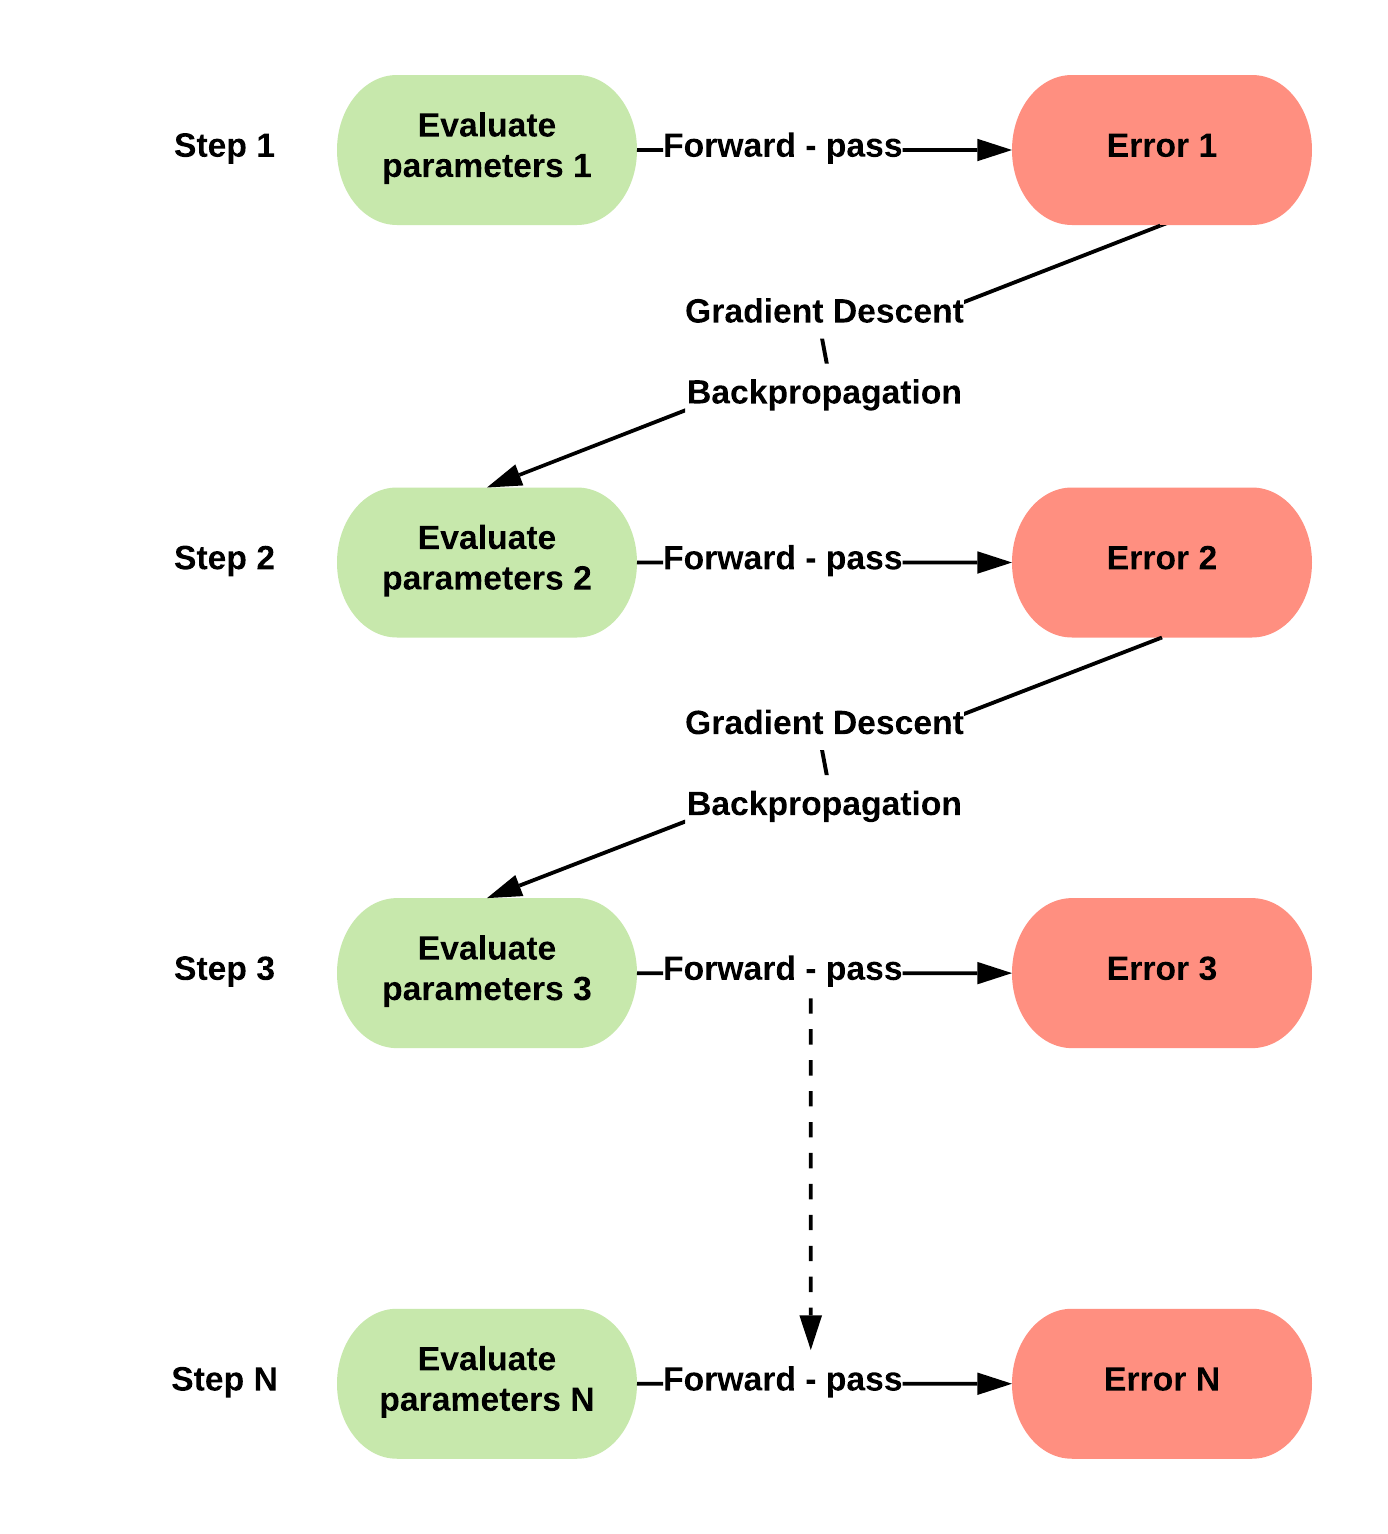
\includegraphics{images/gbem/gradient_descent_informal.png}
    \caption{The process of gradient descent is iterative, and include 3 steps: evaluate the quality of the current parameters (forward-pass step), get the error value, use the error-value in order to update the parameters/getting new set of parameters (back-propagation step). This process is repeated N times, which is decided by either not observing any update in the error, or we ran out of computational resources.}
    \label{fig:grad_descent_inuitive}
\end{figure}

Before we dive into the different optimization methods currently used, it is important first to stress on an important characteristic of all modern deep neural networks, which are \citep{Goodfellow-et-al-2016}:
\begin{itemize}
    \item \textbf{Differentiability}: All the components of the neural networks (activation function, loss objective, regularization, ...etc) are differentiable components. This issue is not about mandatory by theory, but by convenience: good optimizers exist that can use this feature in order to optimize the network faster, while being able to scale with appropriately with the given number of data points and the number of parameters to be optimized.
    \item \textbf{Non-convexity}: While the neural network is built of convex parts, the composition of those parts together is not convex. The reasoning for this particular point is out of the scope of this document. We refer you to the excellent book \citep{Goodfellow-et-al-2016} for more details --. While this seems to be a disadvantage, it is actually a powerful advantage of the neural network. Neural networks are \textit{universal approximator}, meaning that they can approximate/learn any function. A convex function can not approximate non-convex function, but the other way around works \citep{lecture_nn_optimization}.

    Using gradient descent optimization methods in this case leads to convergence to local optima points. The initial conditions of the network (the initial random parameters, and the strategy of their selection) and the optimization strategy and parameters (learning rate, decay factor,...etc) will play an important rule to determine the convergence characteristics (speed of convergence, and local optima) of the neural network.
\end{itemize}

% \subsubsection{Mini-batch optimization}
\par Another important aspect of the success of deep learning is the availability of large amount of data. To optimize a deep neural network (can be the order of millions of parameters) using large amount of data (can be in the order of millions of data examples) using gradient descent, is not physically feasible. We do not have the hardware capability to process all of these data in the same time.

\par To get around this issue, \textit{mini-batch} optimization is used: instead of performing gradient descent based on the information from the whole data, we divide the data into chunks (mini-batches). For each mini-batch, we calculate the loss and the gradient, and update the parameters, and then move on the next batch. The gradient descent in this case is called \textit{Stochastic Gradient Descent}, SGD, \citep{robbins1951stochastic}, following the same equation \ref{eq:grad_descent}, but applied to only a mini-batch at a time, instead of the whole data (batch).

\par Many advances built on top of SGD helped in advancing deep learning, like combining SGD with momentum \citep{rumelhart1988learning}, RMSProp algorithm \citep{hinton2012neural} and Adam algorithm \citep{kingma2014adam}.

%TODO: Not sure if I should keep and expand this part, or no.
% \subsection{Architectures}
% \OSM{INCOMPLETE PART}
%
% In section \ref{sec:RNN}, we discussed the idea behind the basic RNN and its operation. Then, in section \ref{subsec:optimization}, we how we can optimize the parameters of a neural network in general.
%
% \par One important aspect of RNN is the ability to keep the information over many time-steps. This is an issue however with basic RNN networks. This can happen with a better choice of the architecture, that allow to keep the memory, which also learning to select what is not necessary to keep (what we can forget). This problem is called \textit{vanishing gradient}.
%
% A formal discussion for \textit{vanishing gradient} is extensively and better treated in many excellent resources. To get an intuition for it, let's re-phrase what gradient descent optimization is actually doing: the network parameters are evaluated over the data, giving us an error value (the evaluation of the loss function). Using this error value, we move/update the parameters of the network in a direction that minimizes the future error. We keep repeating these steps till we no further improvement is observed (or we exhausted our computational budget). In RNN,
%
% Talk about Vanilla RNN (and what is their problem), LSTMs (and the intuition behind then in solving the problems), and then GRUs (simpler than LSTMs -- fewer parameters --, yet perform similar)

\subsection{Inference: How to generate sequences from the network?}
\par There exists several approaches in order to generate information from the networks. In the case of recurrent neural networks, this is a sequential process (one step at a time, till we generate the whole sequence), as illustrated in figure \ref{fig:text_gen}.

\begin{figure}
    \centering
    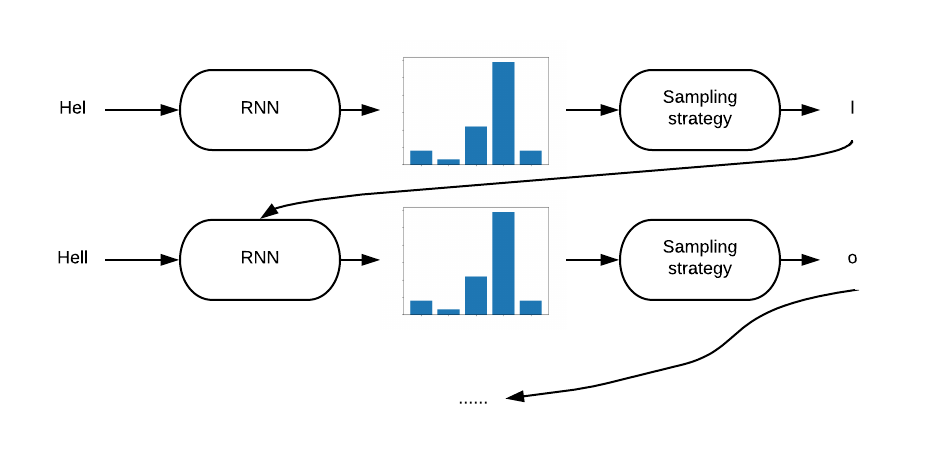
\includegraphics{images/gbem/text_gen.png}
    \caption{An example of using RNN in order to infer a sentence. The token to be generated here is a character. At each time step, the model is given the part of the sentence that has been generated so far, and asked to give the probability distribution over the next character. This distribution is then given to the selected sampling distribution, which sample the next character, and so on.}
    \label{fig:text_gen}
\end{figure}

During the inference mode, the objective is to generate the most likely sequence. We want to solve the following problem

\begin{equation}
    \begin{split}
    \textrm{Find $x_1, x_2, ..., x_N$ that }\\
    {argmax}_{x_1, x_2, ..., x_N}p(x_1, x_2, ..., x_N)
    \label{eq:rnn_obj_inf}
    \end{split}
\end{equation}

% \par Unfortunately, this problem is not tractable, as it scales badly with the number of options (i.e, dimensions) per time step, and the number of time steps required. Multiple methods are being used currently to find an approximate solution to this problem \GB{I would order from the simplest to the most complex}: beam search, temperature sampling, and greedy selection.
% \paragraph{Beam Search} \GB{Describe: selection of N best candidates at each time step of the forward pass given the past and perform a back-pass picking up the best solution}
% \paragraph{Temperature Sampling} \GB{Sample the distribution up to a certain threshold} Since the output of the network is discrete, we use a $SoftMax$ function in order to model this distribution\footnote{The concept of temperature sampling is not limited to the discrete distributions only. You can use it to sample from a \textit{Gaussian Mixture Model} (GMM) for example. In that case, higher temperatures smooth the difference in the weights between the different Gaussian distributions during the sampling process.}.
% \paragraph{Greedy Selection} is a special case of temperature sampling, $T = 0$. In other words, for every time-step, we sample value with the highest probability (e.g., like in the training paradigm). The advantage of this scheme is that it is deterministic and computationally cheap, thus easy to reproduce. The disadvantage on the other side is, like other greedy algorithms, it is sub-optimal, thus yielding worse results.

\par This problem, however, is not tractable, as it scales badly with the number of options (i.e, dimensions) per time step, and the number of time steps required. One simple way is to perform \textit{greedy sampling}, where, at each time step, we select the most likely token. This, however, leads to repetitive and predictable patterns \citep{chollet2017book}.

\par A better way will be to use \textit{stochastic sampling}, by leveraging the fact that at each step, we have a probability distribution over all possible tokens. This allows more diversity in the generated tokens, and also allow unlikely tokens to be sampled some of the time.

\par But what if we want to control the level of randomness in the sampling process? Having such control will allow us to explore different ways to infer from the model, in order to determine the most satisfying way. This control can be done using \textit{temperature sampling}. The idea is to reshape the probability distribution over the different token. On one extreme, very high temperature (going to infinity) will flatten the distribution, making the distribution equivalent to \textit{uniform distribution}. On the other extreme, a temperature of zero will be mount to greedy sampling. This is illustrated in figure \ref{fig:temperature_sampling}.

\begin{sidewaysfigure}[!htbp]
    \centering
    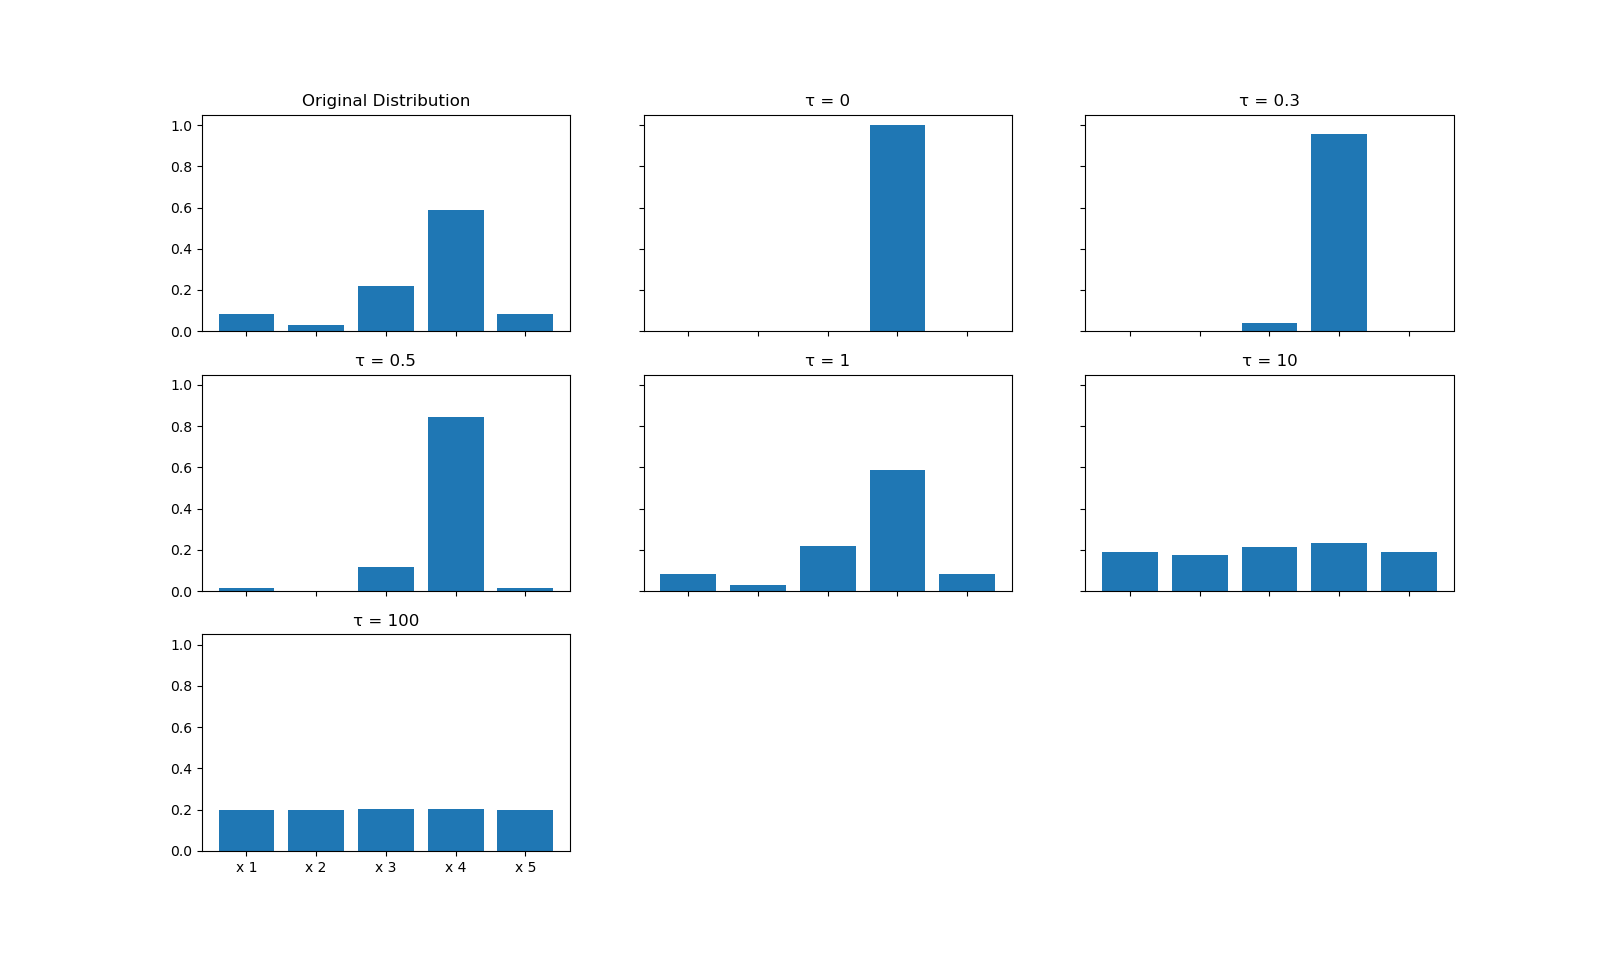
\includegraphics[scale=0.5]{images/gbem/temperature_sampling.png}
    \caption{Illustration of temperature sampling. When the temperature $\tau$ is very low, it becomes greedy sampling. With the increase of temperature, we can see more higher possibility of sampling the lower-probability tokens. When the temperature is too high, it becomes uniform sampling.}
    \label{fig:temperature_sampling}
\end{sidewaysfigure}

\par A clear advantage for temperature sampling is its simplicity, ease of implementation, and ability to generate diverse outputs. However, this also create a challenge when we want to focus on issues like repeatability and reproducibility.

\par Another important thing to notice is that the training/optimization part is not the same as the generation part. Usually in machine learning, there is a symmetry between the training and testing procedures. However, in generation, we are suddenly letting the model generate long sequences, and use it output from the current step as the input to the next step. The model is not trained to see its own output in the input. It is trained to see always the ground truth in the input. Overtime, there is an accumulation of errors that build up, leading to the degradation in the quality of generation \citep{DBLP:journals/corr/RanzatoCAZ15}. This discrepancy between the training and generation will have consequences in the evaluation process, as we will see shortly.

\subsection{How to introduce prior to the model? (conditioning the model)}
\par When training a RNN network, we initialize the first hidden state with zeros. This way, we are informing the model that we are not making any prior assumptions about that particular sequence, and that all sequences in the data have the same 'no prior assumption' condition.

\par However, what if you want to add some prior knowledge about the sequence to the model? There are two reasons why we may want to do that:
\begin{itemize}
    \item Increase accuracy: In case we are doing some classic pattern recognition task (classification, regression), having extra useful information will definitely help increasing the model final performance.
    \item Act as a command: In case of generative model -- during the generative mode -- we need a way to \textit{trigger} the model in order to start generating a sequence in a particular context. For example, we want to tell the model to generate letter 'A'.  Initializing the model with this value allow it to start generating letter A.
\end{itemize}

There are multiple ways to bias the model, all targeting the same thing: initializing the hidden state of the model. Some work in the literature combines multiple of these approaches in the same setup. To the best of my knowledge, there is no one place which all these methods are discussed together.

\paragraph{Initialize the first hidden state directly} This is a common approach, used image captioning \citep{karpathy2015deep}, machine translation, and sequence-to-sequence autoencoders. This is illustrated in figure \ref{subfig:hidden_state}.

\paragraph{Using the first time-step} This method was used in the work done in \citep{vinyals2015show}, in the area of image captioning. The prior in this case is the image, and the objective is to generate the text caption for it. In order to condition the model, the authors projected the image information into the same size as the word embedding used, thus creating a \textit{fake} word, and concatenated this new word with the rest of the words. This is similar to have a word at $X_{-1}$. The hidden state after this fake word is now condition on the information from the image. This is illustrated in figure \ref{subfig:first_timestep}.

\paragraph{Using context sequence -- multiple time-steps --} In this approach, the model is provided with some time-steps from the ground truth, in give it a context. At the end of the these given time-steps, the hidden state is initialized with information about what to be done. A use case for this scenario -- for example -- is when training a language model on multiple authors. When asking the model to generate, you can provide some sentences from the author you want, so the model can follow on this.

\paragraph{Concatenating input time-steps with the condition} In the work done by \citep{ha2017neural}, although not mentioned explicitly, the dataset used -- the \textit{QuickDraw} dataset, discussed earlier -- is quite complicated -- they choose different tasks than us --. It is hard to make the model remember the information about such a complex task over a long time span. Thus, the authors use a mix of \textit{initializing the first hidden state} and \textit{concatenating with the first time-step} in order to make it easier for the model to remember the task. This is illustrated in figure \ref{subfig:cat_timestep}.

\paragraph{Concatenating the hidden state with the condition} This approach is more popular now, since it allows the use of \textit{attention mechanisms} \citep{NIPS2010_4089,denil2012learning}. Examples for this in image captioning \citep{xu2015show}, speech synthesis \citep{wang2017tacotron}.

\begin{figure}
    \centering
    \begin{subfigure}[b]{\textwidth}
      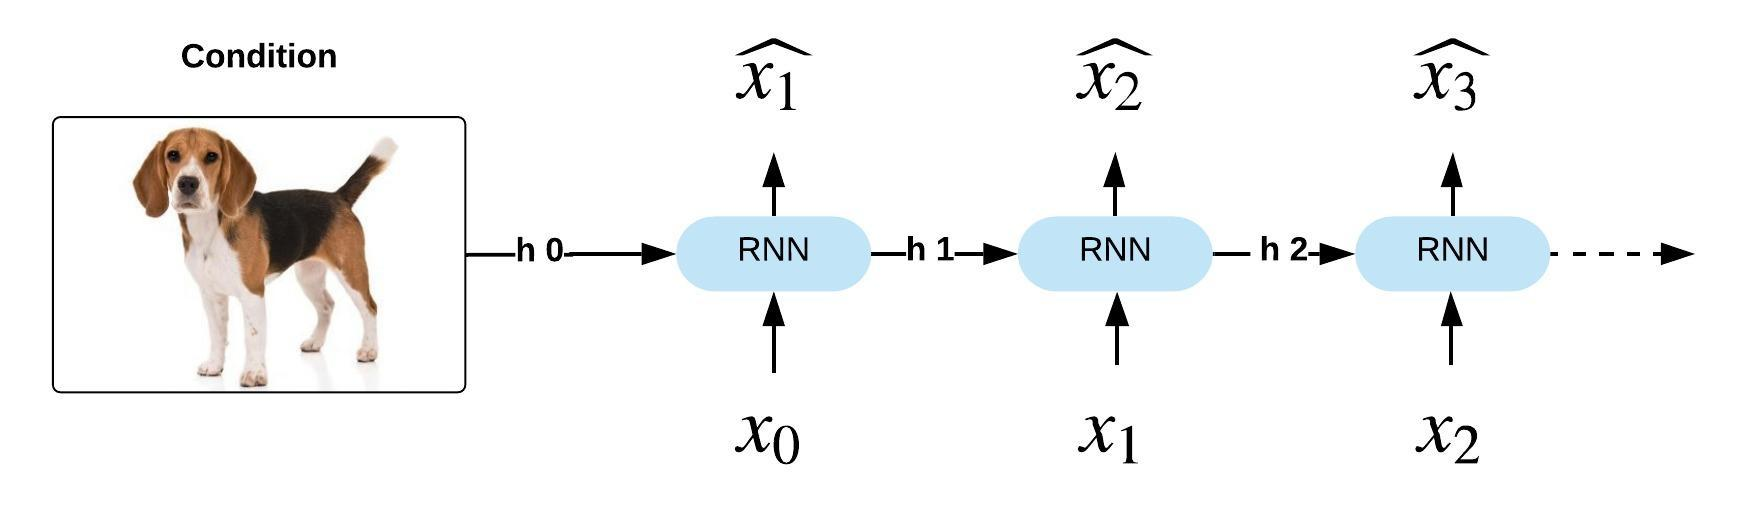
\includegraphics[width=\textwidth]{images/gbem/conditioning_model/hidden_state.jpeg}
      \caption{Initializing the hidden state}
      \label{subfig:hidden_state}
    \end{subfigure}
    ~
    \begin{subfigure}[b]{\textwidth}
        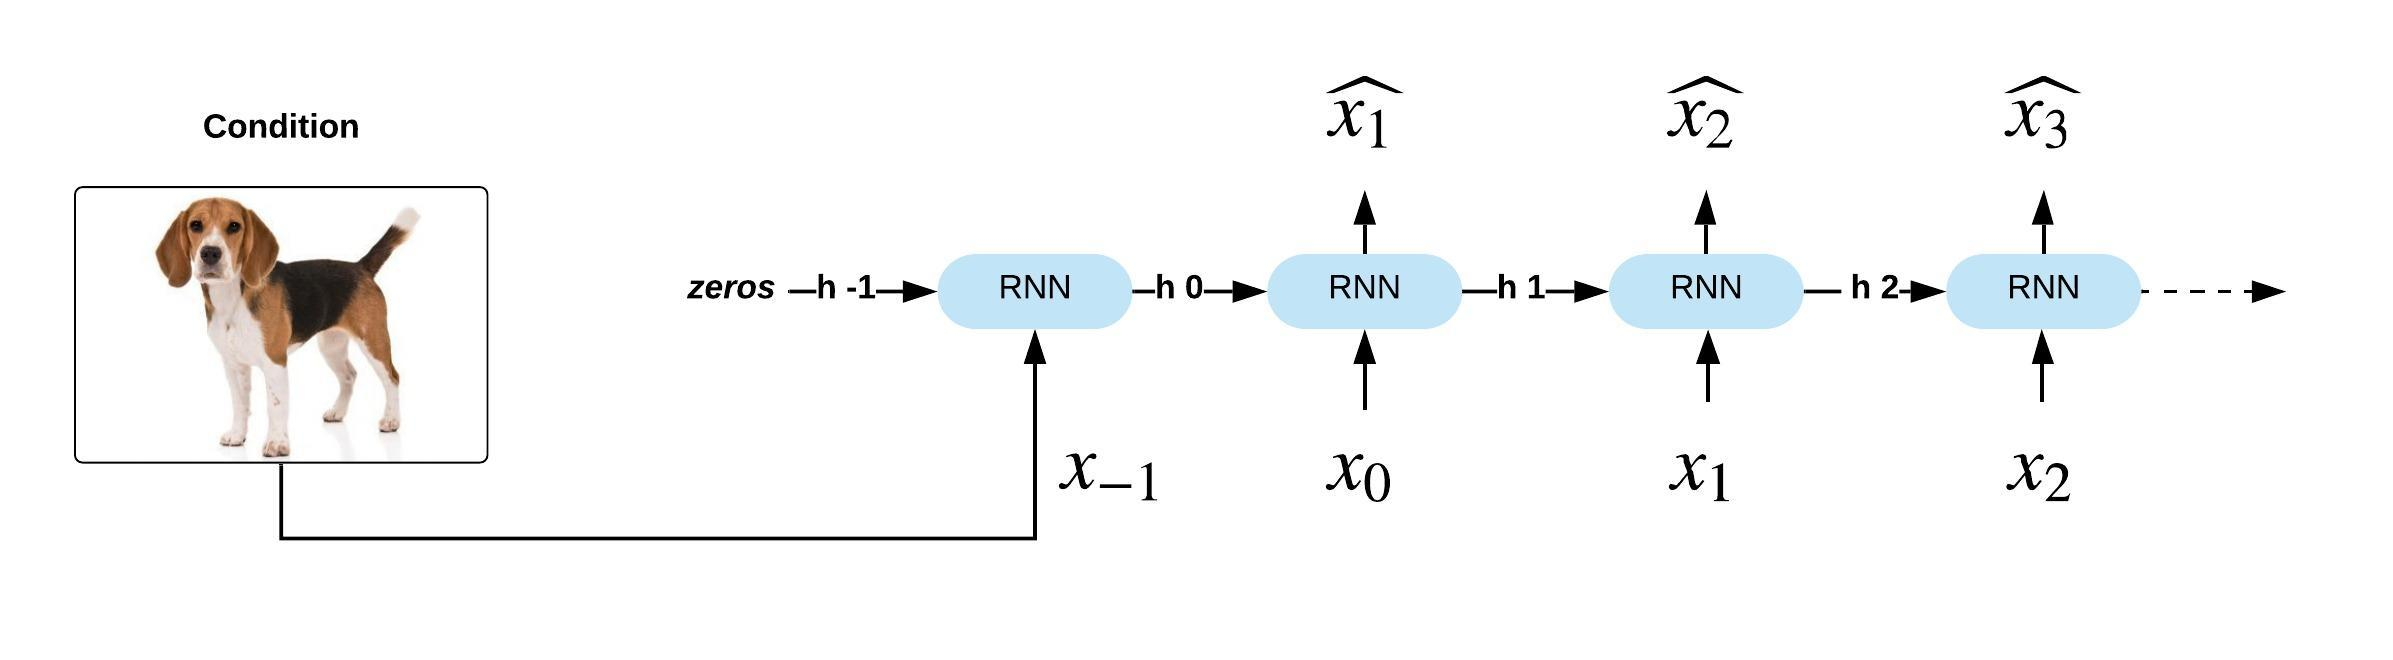
\includegraphics[width=\textwidth]{images/gbem/conditioning_model/first_timestep.jpeg}
        \caption{Initializing using the first time-step}
        \label{subfig:first_timestep}
    \end{subfigure}
    ~
    \begin{subfigure}[b]{\textwidth}
        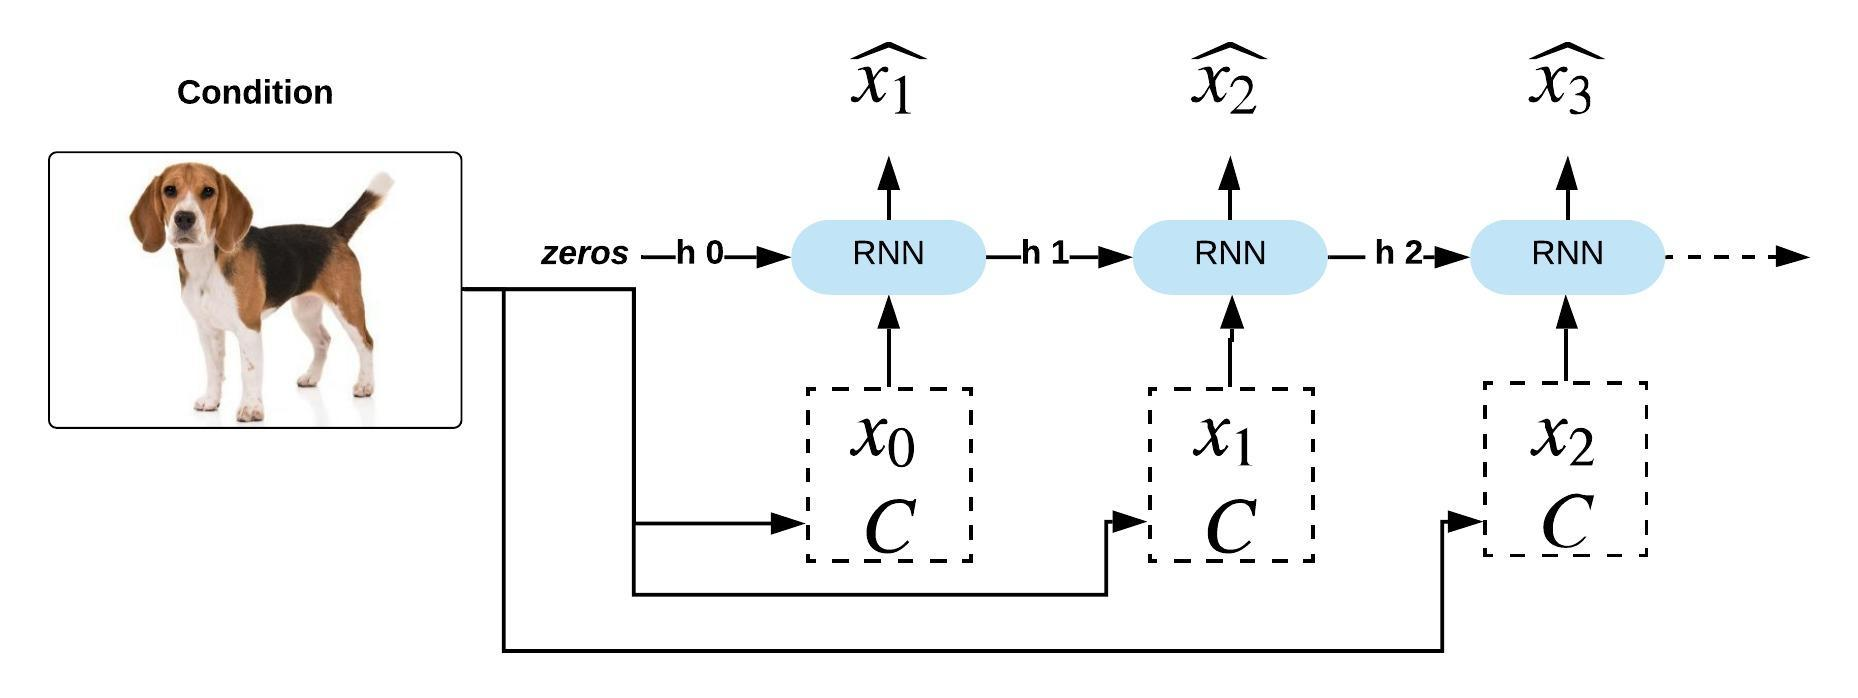
\includegraphics[width=\textwidth]{images/gbem/conditioning_model/cat_timestep.jpeg}
        \caption{Concatenating the condition with time-step}
        \label{subfig:cat_timestep}
    \end{subfigure}
    \caption{Different conditioning method for RNN}
    \label{fig:conditioning_model}
\end{figure}

\subsection{How to evaluate the quality of generation?}\label{sec:eval_metrics}
  % \OSM{INCOMPLETE SUB-SECTION}
  %
  % \textbf{NOTE: Explore this problem in speech and statistical machine translation/text generation.}
  % \begin{itemize}
  %     \item divide into sections: static and temporal data
  %     \item text, speech evaluation
  %     \item using an oracle model (the error concatenation problem, and the adversarial attack).
  % \end{itemize}
  % \par The problem of evaluating the quality of the generation/synthesis process is a challenging task in the domain of generative models.
  \par The objective evaluation of a generative model is a challenging task, since there is no consensus for objective evaluation metrics. We can not simply make strict comparisons between the generated data and the ground truth, since, as we saw earlier in the inference section, there is asymmetry between the training and the generation task. While a subjective evaluation can be a workaround to this problem, it is quite slow, expensive and hinders the development of new models and approaches. The need for objective evaluation that are consistent with the relevant subjective evaluation is thus a necessity.

  \par Let's see how this problem is approached in different domains:
  % In many cases, a subjective evaluation is performed to overcome this problem. For handwriting of Chinese letters, \cite{DBLP:journals/corr/abs-1801-08624} proposed two metrics:
  \begin{description}
    \item [Text] Evaluating text is an essential task to assess the quality of generation in many applications, like image captioning, language translation and language modeling. An example for an objective text evaluation metric is \textit{BLEU score} \citep{papineni2002bleu}, which stands for \textit{bilingual evaluation understudy}, it is a well known metric to evaluate text generation applications, like image captioning \citep{karpathy2015deep,vinyals2015show} and machine translation \citep{Sutskever:2014:SSL:2969033.2969173}. It tries to capture the human evaluation criteria for the quality of the generated text. It compares individual generated segments -- the size of the segments is a parameter to set -- to see if they exist in the ground truth. It does not focus on the location of that segment, just the fact if it exists or not. The small segments -- letters or words -- are used in order to measure the \textit{adequacy} of the generation, while the longer segments are used to measure the \textit{fluency} of the generation. Usually, the metrics is reported on segments from one to four words, to give and overall idea about the quality of the system.

    Other objective metrics were developed and commonly used, such as \textit{METEOR} \citep{denkowski:lavie:meteor-wmt:2014} and \textit{Word Error Rate} \citep{klakow2002testing}.

    \item [Speech synthesis] We are not aware of commonly used objective metrics in this area. A commonly used subjective criteria is Mean opinion score (MOS), which is the average of individuals' opinions on the quality of the system. \textit{Blizzard Challenge} \citep{blizzard} is an annual competition in speech synthesis, to encourage the development of better speech synthesizers. The evaluation is much more detailed that MOS, by trying to assess multiple criteria for speech, like intelligibility, naturalness and the efficiency of the speech in a given domain.

    \item [Handwriting of offline Chinese letters] \cite{DBLP:journals/corr/abs-1801-08624} proposed two metrics to evaluate the quality of their generated letters: content accuracy and style discrepancy. For the first metrics, they train an \textit{evaluator} model on the ground truth data, and use it to recognize the letters produced by their generator. For the second metric, they follow an approach developed in \cite{DBLP:journals/corr/GatysEB15a} -- where the authors studied the problem of image style transfer --, by measuring the correlation between different filter activations (in convolution neural network) at one layer -- which represents the style representation --
  \end{description}

  \par I would like to phrase the objective from these metrics here as \textit{the desire to capture the distance between the generated and the ground truth distribution}. It is not important if some individual mistakes happens in the generated sequence, what matters is to capture the essence of the ground truth distribution.

  \par That being said, for complex distribution, capturing the distribution, or even measuring the distance between two distributions, is not always a tractable task. As noted in the speech synthesis point, sometimes it is better and more practical to consider multiple criteria in the same time in order to better understand and evaluate the behavior of the system. This point will later reflect our decisions concerning the evaluation  criteria for our work.

  % \begin{description}
  %     \item[Content accuracy]: They train an \textit{evaluator} model on the ground truth data, and use it to recognize the letters produced by their generator. This approach however faces important problems: the model is trained with ground truth data, and this results in error in the classification, $E_{eval-ref}$. We call the error of the generator $E_{gen}$. When the evaluator is exposed to the data coming from the generator, a new source/distribution of errors is now coming from the generator, which the evaluator have never been exposed to before, leading to a change in the evaluator error behavior. We call this new error $E_{eval-gen}$. Thus, there are no guarantee that the result of the evaluator is faithful in this case. It is also not possible to deduce $E_{gen}$ from just knowing $E_{eval-ref}$ and $E_{eval-gen}$, since the model performance in this case is unknown.
  %     \item[Style discrepancy]: In \cite{DBLP:journals/corr/GatysEB15a}, the authors performed image style transfer: take an image, and transform it to the style of an artist. In order to evaluate the quality of the transfer, they measured the correlation between different filter activations (in convolution neural network) at one layer -- which represents the style representation --. While this metric is interesting to explore, it is not directly applicable to our case, since it assumes the use of convolution neural network.
  % \end{description}
  %
  % \par \cite{mohammed2018DTL} also addressed the problem of evaluation of handwriting generation. They used the \textit{BLEU score} \cite{papineni2002bleu} (a metric widely used in text translation and image captioning) and the \textit{End of Sequence} (EoS) analysis. They showed that these metrics correlate with the quality of the generated letter.
  %
  % \par The BLEU score is global: all frames of the generated sequence contribute to the final score. The BLEU score is used to compare segments of generated traces with the ground truth. Depending on the number of \textit{grams} chosen, the BLEU score can compare larger segments, thus giving us different levels of granularity to assess the quality of the generated samples.

  % The EoS is a simple yet important style feature. Some letters take longer (i.e. written using many strokes, like H or E) to write than other letters (e.g with one stroke like O or C). It is also an idiosyncratic feature of the writer: writers have different writing speeds, depending on age, education or cognitive/peripheral disorders. We used these metrics in our work as well as a letter-specific metric (applicable only to a subset of the data): the average angular momentum of the letter X will be discussed in detail in the section~\ref{sec:evaluation} below.

  % \par The EoS is a simple yet important style feature. Some letters take longer (e.g., written using many strokes, like H or E) to write than other letters (e.g., written with one stroke like O or C). It is also an idiosyncratic feature of the writer: writers have different writing speeds, depending on age, education or cognitive/peripheral disorders.

\section{Putting it all together}
\par In the previous section, we explored multiple building blocks for the work to come, like recurrent neural networks (architectures, training, inference and conditioning). We also discussed the issue of evaluation the output of generative models, discussing three aspects: evaluation in case of text (image captioning, translation, and text generation in general), speech synthesis, and the dangers of using another model (oracle model) in order to evaluate the generation quality.

\par In this section, I discuss how to put all these elements together, the decisions made, and the experimental setup used, in order to address the following three questions:
\begin{itemize}
    \item How to generate handwritten letters using deep learning framework?
    \item How to evaluate the generated traces?
    \item What benchmarks are suitable to compare to?
\end{itemize}

\subsection{Our proposed evaluation metrics}\label{subsec:eval_metrics}
\par As discussed earlier, evaluation is a challenging problem when using generative models. We want metrics to capture the distance between the generated and the ground truth distributions. We propose using the following metrics:

\paragraph{BLEU score} As mentioned earlier, BLEU score is used in the evaluation of text generation. Since we discretized the letter drawings, this fits nicely within our work. The general intuition is the following: if we take a segment from the generated letter, did this segment happen in the ground truth letter? We keep doing this for segments of increasing length (the length of the segment here is the number of grams used in the BLEU score). For our work, we report the results on segments from 1 to 3 time steps.

Each part of the letter has two parallel segments: freeman codes and speed, thus, we report the BLEU score for both of them.
The equation to compute the BLEU score is the following:
\begin{equation}
BLEU_{N} = \frac{\sum_{C\in G}\sum_{N\in C}Count_{Clipped}(N)}{\sum_{C\in G}\sum_{N\in C}Count(N)}
\end{equation}
\begin{equation}
Score_{N} = \min{(0, 1 - \frac{L_{R}}{L_{G}})} \prod^{N}_{n=1}BLEU_{n}
\end{equation}

where: $G$ is all the generated sequences, $N$ is the total number of N-grams we want to consider. $Count_{Clipped}$ is clipped N-grams count (if the number of N-grams in the generate sequence is larger than the reference sequence, the count is limited to the number in the reference sequence only), $L_R$ is the length of the reference sequence, $L_G$ is the length of the generated sequence.
The term $\min(0, 1 - \frac{L_{R}}{L_{G}})$ is added in order to penalize short generated sequences (shorter than the reference sequence), which will deceptively achieve high scores.

\par In order to get into the intuition of using such a metric in evaluating the quality of handwriting generation, we can imagine that we are comparing segments of a generated trace to segments in the ground truth letter, by asking the following question: does the segment in the generated trace exist (anywhere) in the original trace? The shorter segments represent \textit{adequacy} (i.e., does the generated trace use the same elementary moves like the ground truth trace). The longer segments represents \textit{fluency} of drawing (i.e., how good the drawing is)\footnote{This last interpretation of short and long segments is adapted from the \citep{papineni2002bleu}, which uses them for text translation evaluation.}. See figure \ref{fig:bleu_score}.

\begin{figure}[!htbp]
    \centering
    \begin{subfigure}{0.3\textwidth}
        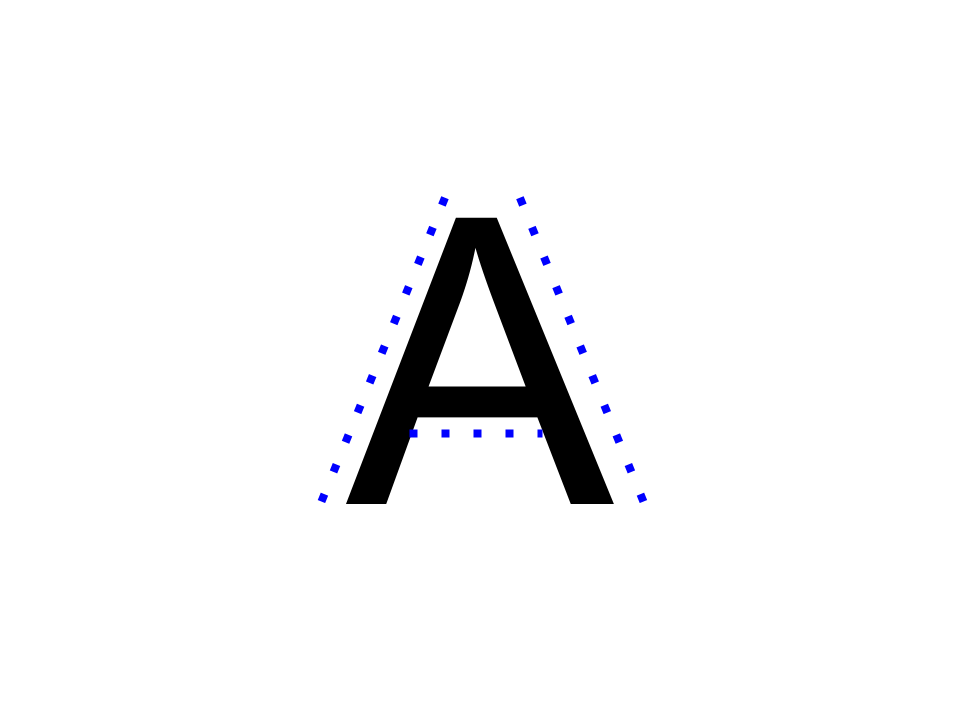
\includegraphics[scale=0.3, trim={10cm 7cm 10cm 7cm},clip]{images/gbem/bleu_score_1.png}
    \end{subfigure}
    ~
    \begin{subfigure}{0.3\textwidth}
        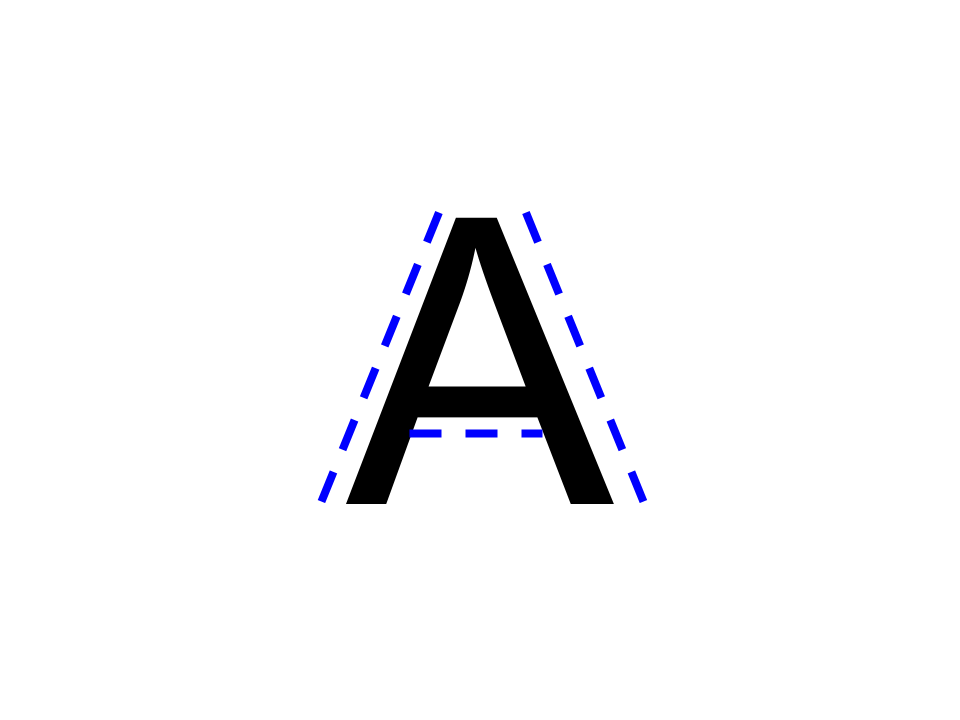
\includegraphics[scale=0.3, trim={10cm 7cm 10cm 7cm},clip]{images/gbem/bleu_score_2.png}
    \end{subfigure}
    ~
    \begin{subfigure}{0.3\textwidth}
        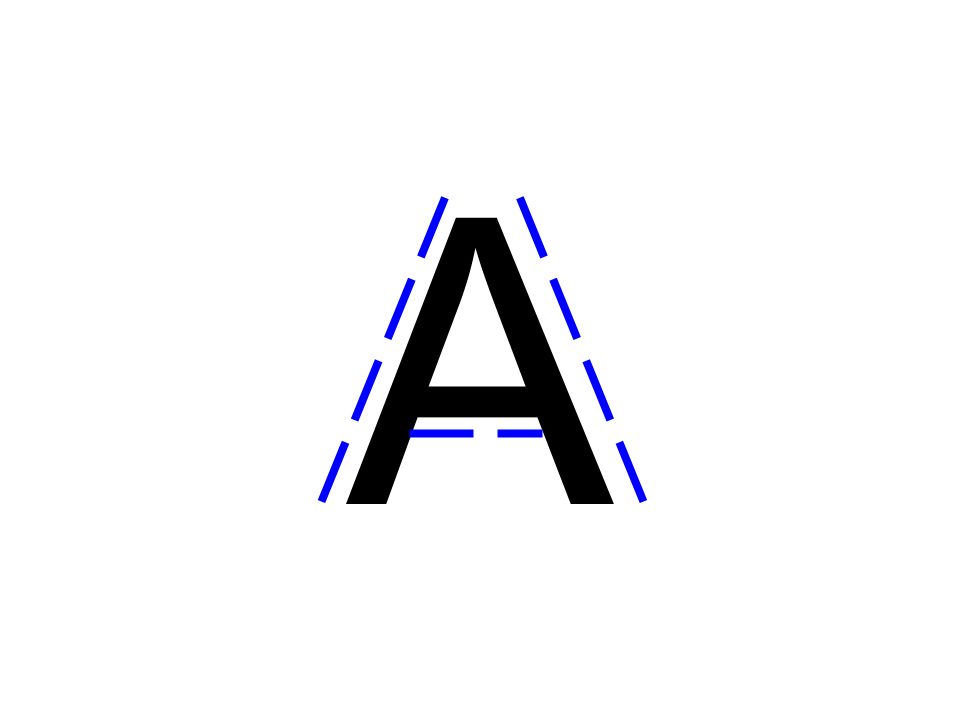
\includegraphics[scale=0.3, trim={10cm 7cm 10cm 7cm},clip]{images/gbem/bleu_score_3.png}
    \end{subfigure}

    \caption{Using BLEU score of different sizes, we compare segments of variable length in the generated trace to the target trace.}
    \label{fig:bleu_score}
\end{figure}

\paragraph{End of Sequence} The length of the letter is another aspect of the style. The distribution of length in the generated examples should follow the ground truth examples. In order to perform this analysis, we compute ~\textit{Pearson correlation coefficient} between the generated examples and the ground truth data.

\subsection{How to ground the metrics?}\label{subsec:ground_metrics}
\par We assess multiple methods to condition our handwritten letter generator, and evaluate their ability to capture of writing styles. We know their cardinal order of the power of these methods (depends on the kind of information available to each method). Knowing this information beforehand, we can use it to ground our performance metrics. The methods are:
\begin{description}
    \item[Letter identity] the letter id only is used as bias. No style information is thus included. The model will try to average over the different example for the same letter. We consider this as a lower baseline.
    \item[Letter + Writer identities] the letter id and writer id are used as a bias. Thus, the model has an explicit access information about the writer. This method is expected to perform the best. This model will also serve as a upper baseline.
% \end{description}
% \par Starting from the images of the letters, we wanted to test if we can extract information about the style. We two approaches, based on deep learning framework:
% \begin{description}[noitemsep]
    \item[Image classifier embedding] We train a convolution neural network (CNN) to classify the letters images\footnote{This letter classification task achieves $95.1\%$ classification accuracy, which we consider very good.}, as shown in figure~\ref{fig:architectures}. We use an intermediate layer as to extract embeddings, that will encode information about the letter images. This model should perform the same or a more performance than using the letter identity only, since it learns to clusters the letters, and there are classification errors. But we expect it to perform less than the letter + writer identities.
    \item[Image auto-encoder latent space] we train a letter image autoencoder, using reconstruction error, and use the latent space as a representation of the letter + style. The architecture we use can be seen in figure~\ref{fig:architectures}. The latent space encodes the similarity between the letters. This model should perform worse than using the letter identity only, since, while it capture the similarity between the letter images, it does not capture discriminative features about each letter itself.
\end{description}

\par From this discussion, we can say that cardinal power of the different conditions is:
% \begin{subequations}
\begin{align}
    & autoencoder < letter \leq classifier < letter+writer
    \label{eq:cardinal_power}
\end{align}
% \end{subequations}

\begin{figure}[!htbp]
    \centering
    \begin{subfigure}{0.4\textwidth}
        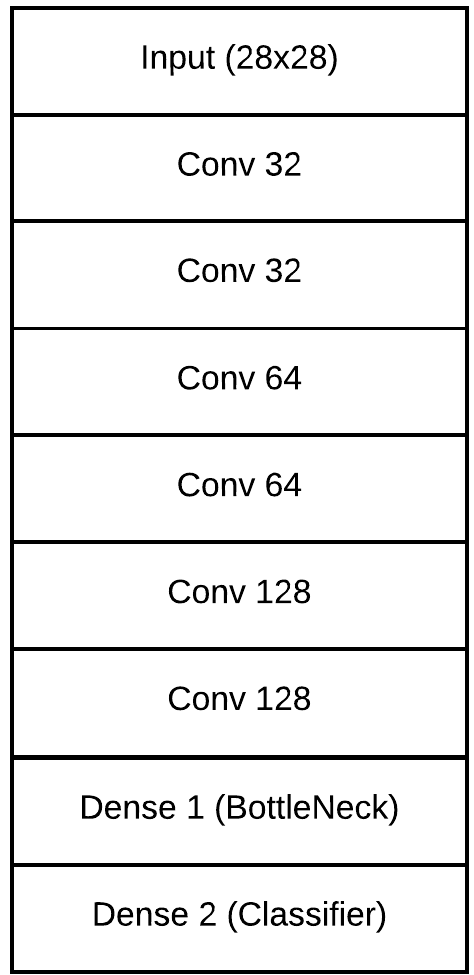
\includegraphics[scale=1.0]{images/gbem/classifier.png}
    \end{subfigure}
    ~
    \begin{subfigure}{0.4\textwidth}
        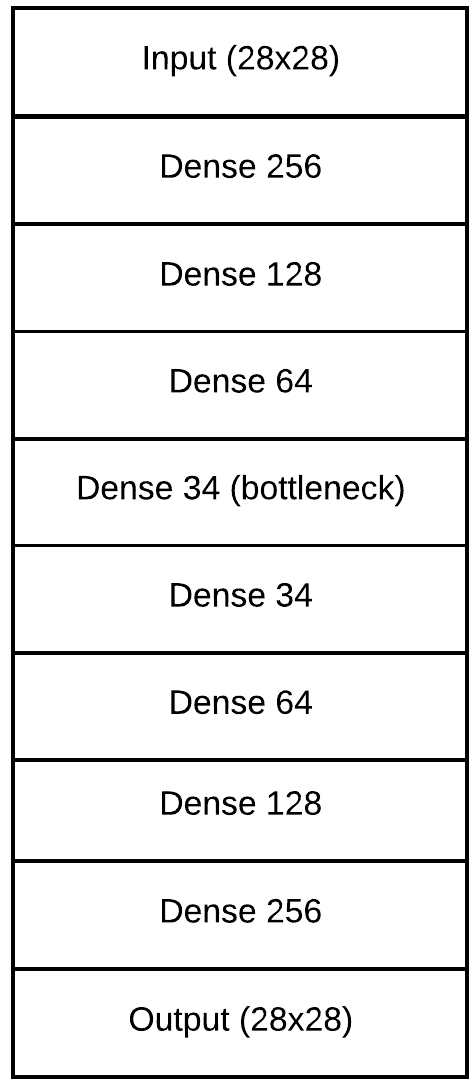
\includegraphics[scale=1.0]{images/gbem/autoenc.png}
    \end{subfigure}
    \caption{Left: architecture of the CNN letter classifier. Batch normalization is used after each convolution layer. The \textit{Dense 1} layer is the embedding that is used to condition our generator. Right: the autoencoder architecture we used. The first \textit{Dense 34} layer provides the latent space used to condition the generator.}
    \label{fig:architectures}
\end{figure}

\subsection{Model proposed}
We use a type of RNN called Gated-Recurrent Network (GRU) \citep{chung2014empirical}, which is known for having a better memory ability than basic RNN, thus, making it suitable choice for long sequence. Our model is a conditioned-GRU model, demonstrated in figure \ref{fig:dtl_model}. Using this model, we compare different style approached discussed in section \ref{subsec:ground_metrics}, and use the generation results from that model in order to ground the proposed evaluation metrics, discussed in section \ref{subsec:eval_metrics}.
\begin{figure}[!htbp]
    \centering
    \begin{subfigure}[b]{\textwidth}
        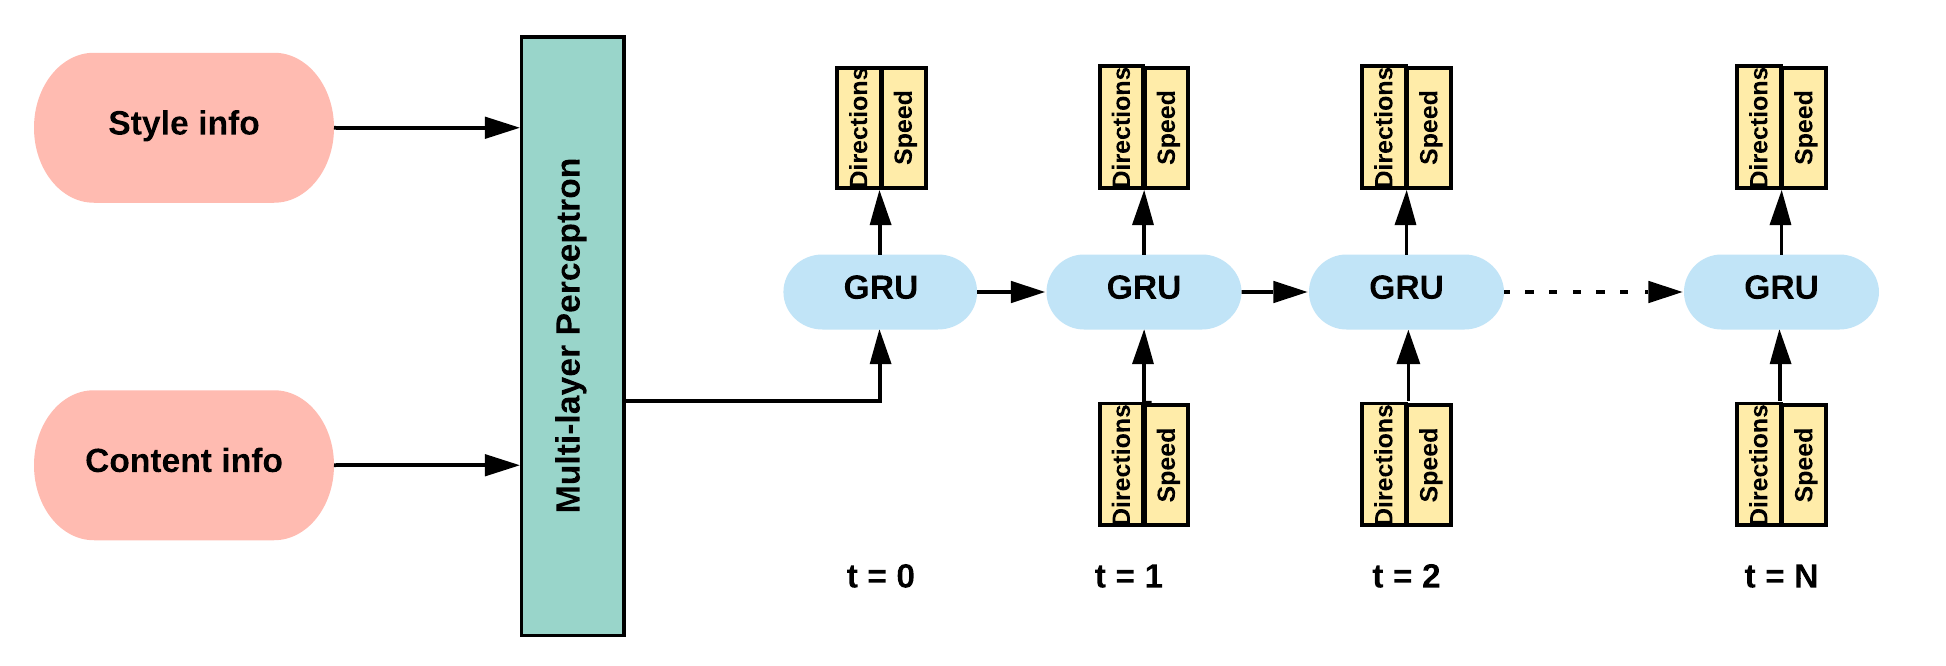
\includegraphics[width=\textwidth]{images/gbem/dtl_training.png}
        \caption{Training mode}
        \label{subfig:dtl_training}
    \end{subfigure}
    ~
    \begin{subfigure}[b]{\textwidth}
        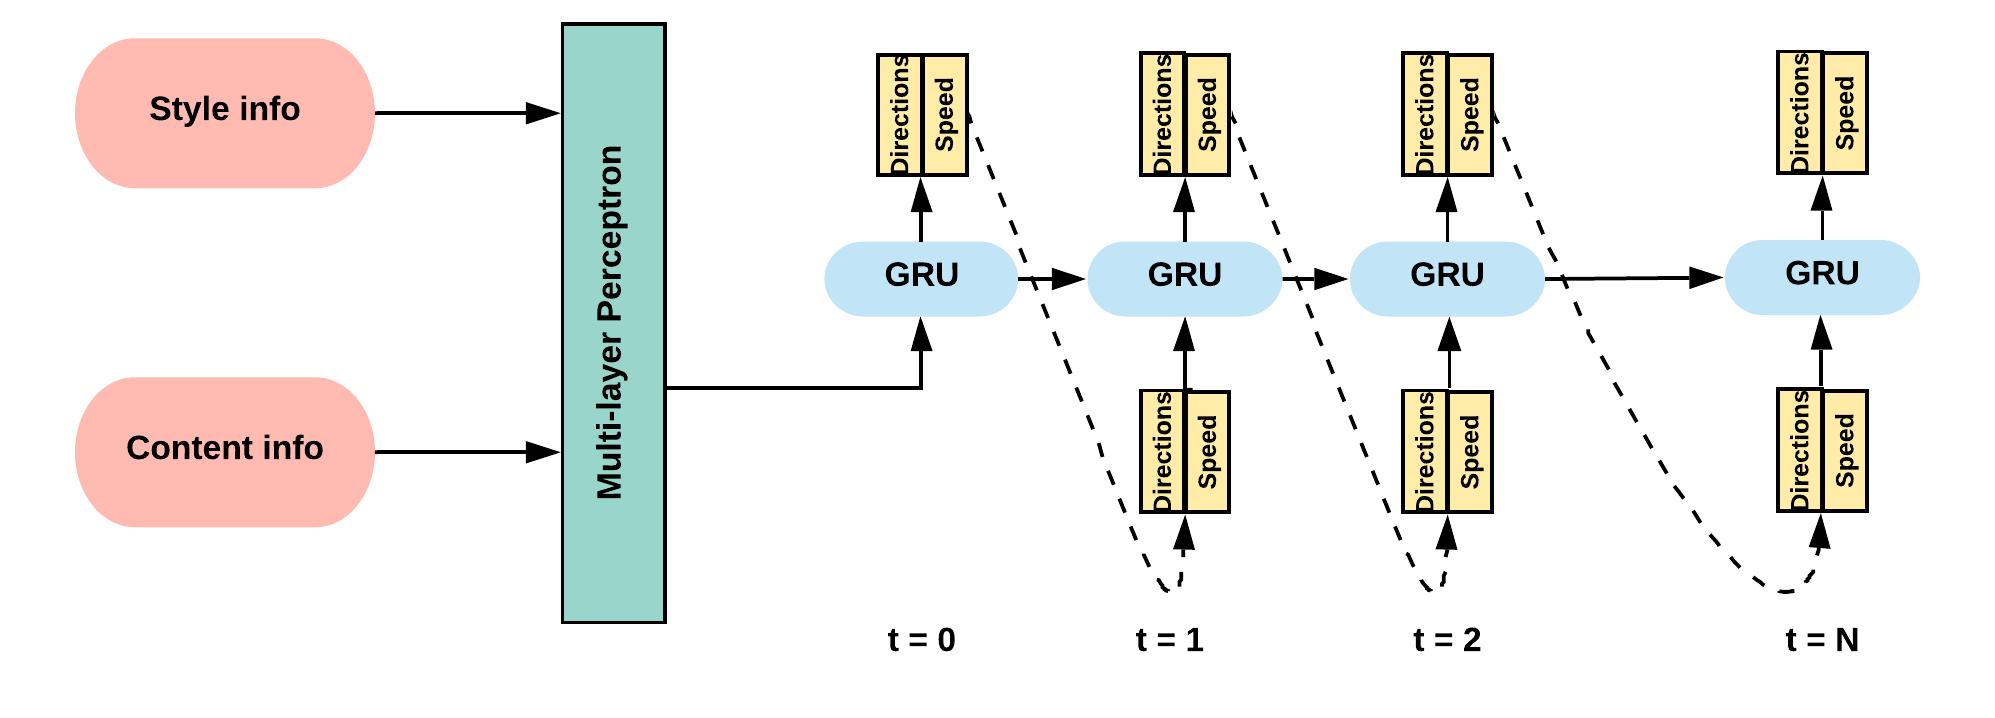
\includegraphics[width=\textwidth]{images/gbem/dtl_generation.png}
        \caption{Generation mode}
        \label{subfig:dtl_generation}
    \end{subfigure}

    \caption{The conditioned-GRU model used in this work. During the training mode \ref{subfig:dtl_training}, the input of the model is always the ground truth, and the predicted value is compared to the ground truth. During the generation mode \ref{subfig:dtl_generation}, the input to the model at each step is the model prediction from the previous step. The 'style info' and the 'task info' inputs are separated here for demonstration (they could be mixed).}
    \label{fig:dtl_model}
\end{figure}

\subsection{Results}
\par We train our different models and generate the traces from them as explained earlier. In this section, we compare the different models using the evaluation metrics discussed before. We  observe the consistency of the reported metrics with the prior information about the cardinal power of the different methods, equation \ref{eq:cardinal_power}. This is how we ground our metrics.

\subsubsection{BLEU score}
\par The final results using the BLEU score can be seen in table \ref{table:1}. The results vary when measuring BLEU-1. But, as we increase the number of grams, BLEU-2 and BLEU-3, to measure the similarity between larger segments of the traces, we can observe:
\begin{itemize}
    \item The letter + writer condition performed better than all other conditions, thus showing that having access to information about the writer, like the writer id, improve the quality of the handwriting synthesis.
    \item The image classifier condition performs better than the letter identity only, but less than the letter + writer bias. Since the classifier is trained on a single objective only (to classify the letters), and the classifier performs well, we expect the embedding to cluster the letters well, as seen in figure \ref{fig:classifier_latent}. We can expect the model to capture some of the writer style, possibly in the inter-cluster variance. This is an interesting result, suggesting that some fine tuning for the image classifier while in the generation task could be beneficial to capture more details about the styles.
    \item The image autoencoder bias performed the worst. To understand why, we plot a 2-D projection of its latent space using t-SNE \citep{maaten2008visualizing}, figure~\ref{fig:autoenc_latent}. Since the autoencoder is trained to minimize the reconstruction error, the distance in the latent space encode the proximity between the images. It can be observed also that this latent space does not encode discriminative features for the letters. Using this latent space for our generator, we find the model gets confused between nearby letters, resulting sometimes in generating different letters than requested.
\end{itemize}

\begin{table}[!htbp]
\centering
\begin{tabular}{|c||c|c|c||c|c|c|}
\hline
\multicolumn{1}{|c||}{Aspect/Feature} & \multicolumn{3}{c||}{ Speed } & \multicolumn{3}{c|}{ Freeman }   \\
\hline
Model / B-score      & B-1  & B-2  & B-3           & B-1  & B-2   & B-3              \\ \hline
Letter identity          & 49.7 & 37.3 & 24.2          & 47.4 & 36.6  & 26.8               \\\hline
Image classifier     & 50.9 & 38.2 & 24.6          & 48.5 & 37.9 & 28.1             \\\hline
Image autoencoder    & \textbf{51.9} & 37.9 & 23.1          & 46.4 & 35.0  & 24.5             \\\hline
\textbf{Letter + Writer identities} & 51.5 & \textbf{41.4} & \textbf{25.1}          & \textbf{56.7} & \textbf{39.4}  & \textbf{28.3}             \\\hline
\end{tabular}
\caption{Comparing different approaches for style extraction using clipped n-grams}
\label{table:1}
\end{table}

\begin{sidewaysfigure}[!htbp]
    \centering
    \begin{subfigure}[b]{0.6\textwidth}
        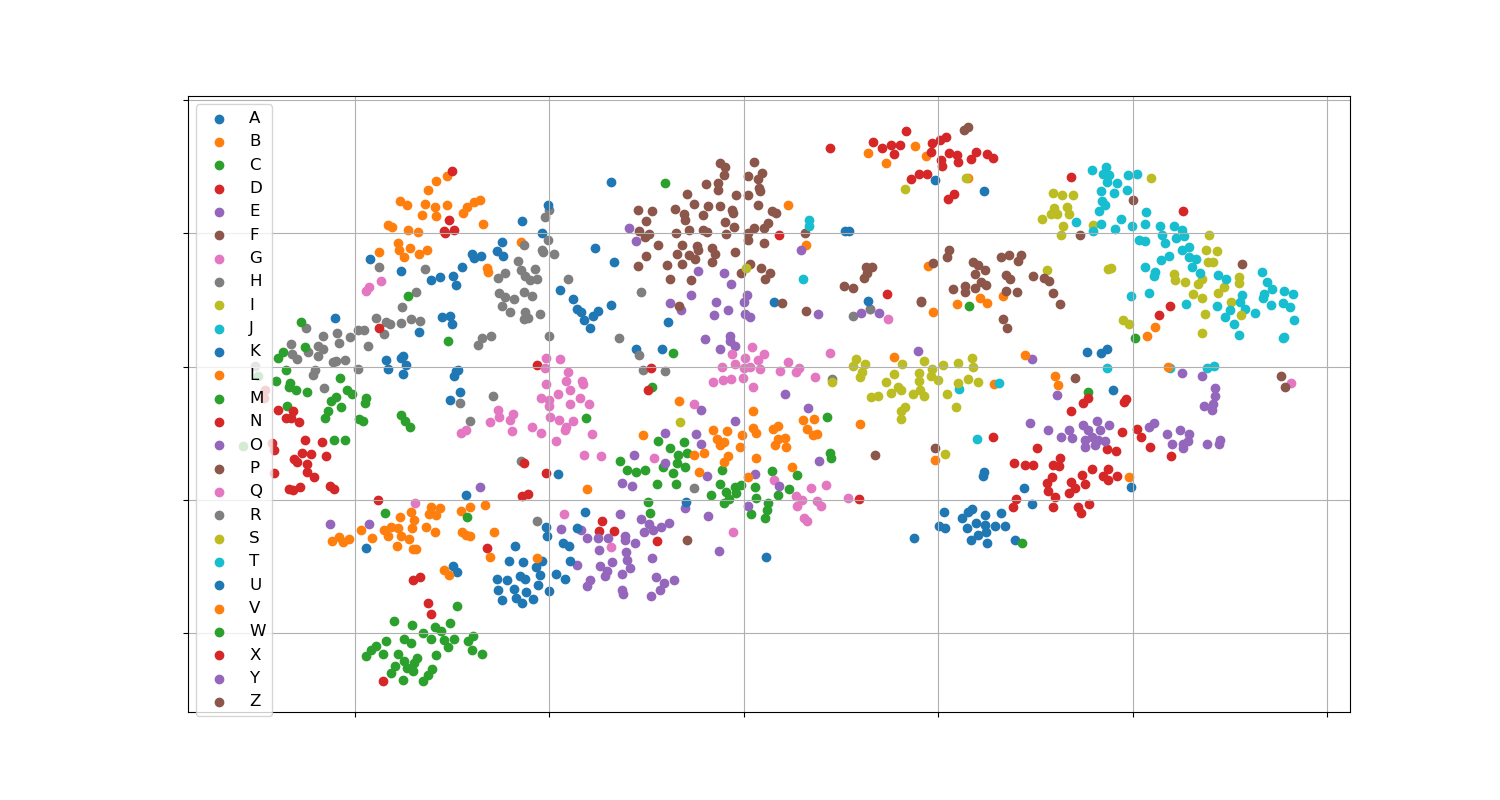
\includegraphics[width=\textwidth]{images/gbem/AutoEnc_Vis_tsne.png}
        \caption{}
        \label{fig:autoenc_latent}
    \end{subfigure}
    % ~
    \quad
    \begin{subfigure}[b]{0.6\textwidth}
        \includegraphics[width=\textwidth]{images/gbem/Classifier_Vis_tsne.png}
        \caption{}
        \label{fig:classifier_latent}
    \end{subfigure}
    % \caption{Shape of the autoencoder latent space. Left: each color represent one letter. Right: labeling for some of the letters, to illustrate proximity.}
    % \includegraphics[width=\textwidth]{figures/AutoEnc_Vis_tsne.png}
    \caption{a) In the the autoencoder latent space, there is no clear separation between letters; the encoding is based on the similarity of the images only. b) In the classifier embedding, there is a clear separation between the letters - with few exceptions -.}

\end{sidewaysfigure}

\subsubsection{Sequence length}
\par As mentioned earlier, we performed a statistical test between the paired distributions of lengths of the generated and the reference tracings. The results are shown in table~\ref{table:2}. We can see the following:
\begin{itemize}
    \item The results from the statistical test shows that the letter + writer bias outperform the rest of the biases, achieving p-value $< 0.05$. This is quite reassuring, since it is also in line with the results from the BLEU score.
    \item The results from the Pearson correlation coefficients are also consistent with the rest of the results. High coefficients are given to the letter + writer bias, compared to the other methods. The image classifier and autoencoder gives the lowest results. This could be due to insufficient information about the letter length that can be inferred from the image. For the image classifier, as noted earlier, a fine-tuning during the generation task is worth exploring.
\end{itemize}

\begin{table}[!htbp]
\centering
\begin{tabular}{|c|c|c|}
\hline
Models & Pearson coefficient & p-value \\ \hline
Letter bias & 0.38 & 0.84 \\ \hline
Image classifier & 0.32 & 0.62\\ \hline
Image autoencoder & 0.25 & 0.29 \\ \hline
\textbf{Letter + Writer bias} & \textbf{0.55} & \textbf{0.04}\\ \hline
\end{tabular}
\caption{Pearson correlation coefficients and associated p-values for the EOS distributions of the different style biases.}

\label{table:2}
\end{table}

\subsection{Examples of the generated letters}
\par The design choices of our experiments (discretization, and ignoring the pen state) affects the final shape of the letters, yet, the letters and their style are quite recognizable. See examples for the original letters in figure \ref{fig:orig_letters_examples}. Examples for the generation with our methods are in figure \ref{fig:letters_examples_gbem}. This is a subjective indication that our model is working properly, producing real-like comprehensible letters.

\begin{sidewaysfigure}%[!htbp]
\centering
    \begin{subfigure}[b]{0.14\textwidth}
        \includegraphics[width=\textwidth]{images/gbem/orig_letters_fig/AORIG_letter_A_writer_8.png}
        \caption{B}
    \end{subfigure}
    ~
    \begin{subfigure}[b]{0.14\textwidth}
        \includegraphics[width=\textwidth]{images/gbem/orig_letters_fig/AORIG_letter_B_writer_7.png}
        \caption{C}
    \end{subfigure}
    ~
    \begin{subfigure}[b]{0.14\textwidth}
        \includegraphics[width=\textwidth]{images/gbem/orig_letters_fig/AORIG_letter_C_writer_5.png}
        \caption{D}
    \end{subfigure}
    ~
    \begin{subfigure}[b]{0.14\textwidth}
        \includegraphics[width=\textwidth]{images/gbem/orig_letters_fig/AORIG_letter_D_writer_6.png}
        \caption{A}
    \end{subfigure}
    ~ %add desired spacing between images, e. g. ~, \quad, \qquad, \hfill etc.
      %(or a blank line to force the subfigure onto a new line)
    \begin{subfigure}[b]{0.14\textwidth}
        \includegraphics[width=\textwidth]{images/gbem/orig_letters_fig/AORIG_letter_E_writer_6.png}
        \caption{E}
    \end{subfigure}
    ~
    \begin{subfigure}[b]{0.14\textwidth}
        \includegraphics[width=\textwidth]{images/gbem/orig_letters_fig/AORIG_letter_F_writer_4.png}
        \caption{F}
    \end{subfigure}
    ~
    \begin{subfigure}[b]{0.14\textwidth}
        \includegraphics[width=\textwidth]{images/gbem/orig_letters_fig/AORIG_letter_G_writer_5.png}
        \caption{G}
    \end{subfigure}
    ~
    \begin{subfigure}[b]{0.14\textwidth}
        \includegraphics[width=\textwidth]{images/gbem/orig_letters_fig/AORIG_letter_H_writer_16.png}
        \caption{H}
    \end{subfigure}
    ~
    \begin{subfigure}[b]{0.14\textwidth}
        \includegraphics[width=\textwidth]{images/gbem/orig_letters_fig/AORIG_letter_I_writer_5.png}
        \caption{I}
    \end{subfigure}
    ~
    \begin{subfigure}[b]{0.14\textwidth}
        \includegraphics[width=\textwidth]{images/gbem/orig_letters_fig/AORIG_letter_J_writer_4.png}
        \caption{J}
    \end{subfigure}
    ~
    \begin{subfigure}[b]{0.14\textwidth}
        \includegraphics[width=\textwidth]{images/gbem/orig_letters_fig/AORIG_letter_K_writer_4.png}
        \caption{K}
    \end{subfigure}
    ~
    \begin{subfigure}[b]{0.14\textwidth}
        \includegraphics[width=\textwidth]{images/gbem/orig_letters_fig/AORIG_letter_L_writer_16.png}
        \caption{L}
    \end{subfigure}
    ~
    \begin{subfigure}[b]{0.14\textwidth}
        \includegraphics[width=\textwidth]{images/gbem/orig_letters_fig/AORIG_letter_M_writer_10.png}
        \caption{M}
    \end{subfigure}
    ~
    \begin{subfigure}[b]{0.14\textwidth}
        \includegraphics[width=\textwidth]{images/gbem/orig_letters_fig/AORIG_letter_N_writer_1.png}
        \caption{N}
    \end{subfigure}
    ~
    \begin{subfigure}[b]{0.14\textwidth}
        \includegraphics[width=\textwidth]{images/gbem/orig_letters_fig/AORIG_letter_O_writer_2.png}
        \caption{O}
    \end{subfigure}
    ~
    \begin{subfigure}[b]{0.14\textwidth}
        \includegraphics[width=\textwidth]{images/gbem/orig_letters_fig/AORIG_letter_P_writer_11.png}
        \caption{P}
    \end{subfigure}
    ~
    \begin{subfigure}[b]{0.14\textwidth}
        \includegraphics[width=\textwidth]{images/gbem/orig_letters_fig/AORIG_letter_Q_writer_4.png}
        \caption{Q}
    \end{subfigure}
    ~
    \begin{subfigure}[b]{0.14\textwidth}
        \includegraphics[width=\textwidth]{images/gbem/orig_letters_fig/AORIG_letter_R_writer_2.png}
        \caption{R}
    \end{subfigure}
    ~
    \begin{subfigure}[b]{0.14\textwidth}
        \includegraphics[width=\textwidth]{images/gbem/orig_letters_fig/AORIG_letter_S_writer_1.png}
        \caption{S}
    \end{subfigure}
    ~
    \begin{subfigure}[b]{0.14\textwidth}
        \includegraphics[width=\textwidth]{images/gbem/orig_letters_fig/AORIG_letter_T_writer_1.png}
        \caption{T}
    \end{subfigure}
    ~
    \begin{subfigure}[b]{0.14\textwidth}
        \includegraphics[width=\textwidth]{images/gbem/orig_letters_fig/AORIG_letter_U_writer_5.png}
        \caption{U}
    \end{subfigure}
    ~
    \begin{subfigure}[b]{0.14\textwidth}
        \includegraphics[width=\textwidth]{images/gbem/orig_letters_fig/AORIG_letter_V_writer_11.png}
        \caption{V}
    \end{subfigure}
    ~
    \begin{subfigure}[b]{0.14\textwidth}
        \includegraphics[width=\textwidth]{images/gbem/orig_letters_fig/AORIG_letter_W_writer_2.png}
        \caption{W}
    \end{subfigure}
    ~
    \begin{subfigure}[b]{0.14\textwidth}
        \includegraphics[width=\textwidth]{images/gbem/orig_letters_fig/AORIG_letter_X_writer_5.png}
        \caption{X}
    \end{subfigure}
    ~
    \begin{subfigure}[b]{0.14\textwidth}
        \includegraphics[width=\textwidth]{images/gbem/orig_letters_fig/AORIG_letter_Y_writer_5.png}
        \caption{Y}
    \end{subfigure}
    ~
    \begin{subfigure}[b]{0.14\textwidth}
        \includegraphics[width=\textwidth]{images/gbem/orig_letters_fig/AORIG_letter_Z_writer_15.png}
        \caption{Z}
    \end{subfigure}

    \caption{Examples of original letters. The blue \textit{x} mark is the starting point. These ones are generated using the letter + Writer bias. E and F are visually harder to recognize, since we do not model the pen pressure, otherwise, the rest of the letters are well recognizable.}\label{fig:orig_letters_examples}
\end{sidewaysfigure}

\begin{sidewaysfigure}[!htbp]
\centering
    \begin{subfigure}[b]{0.14\textwidth}
        \includegraphics[width=\textwidth]{images/gbem/letters_generated/A.png}
        \caption{A}
    \end{subfigure}
    ~ %add desired spacing between images, e. g. ~, \quad, \qquad, \hfill etc.
      %(or a blank line to force the subfigure onto a new line)
    \begin{subfigure}[b]{0.14\textwidth}
        \includegraphics[width=\textwidth]{images/gbem/letters_generated/B.png}
        \caption{B}
    \end{subfigure}
    ~
    \begin{subfigure}[b]{0.14\textwidth}
        \includegraphics[width=\textwidth]{images/gbem/letters_generated/C.png}
        \caption{C}
    \end{subfigure}
    ~
    \begin{subfigure}[b]{0.14\textwidth}
        \includegraphics[width=\textwidth]{images/gbem/letters_generated/D.png}
        \caption{D}
    \end{subfigure}
    ~
    \begin{subfigure}[b]{0.14\textwidth}
        \includegraphics[width=\textwidth]{images/gbem/letters_generated/E.png}
        \caption{E}
    \end{subfigure}
    ~
    \begin{subfigure}[b]{0.14\textwidth}
        \includegraphics[width=\textwidth]{images/gbem/letters_generated/F.png}
        \caption{F}
    \end{subfigure}
    ~
    \begin{subfigure}[b]{0.14\textwidth}
        \includegraphics[width=\textwidth]{images/gbem/letters_generated/G.png}
        \caption{G}
    \end{subfigure}
    ~
    \begin{subfigure}[b]{0.14\textwidth}
        \includegraphics[width=\textwidth]{images/gbem/letters_generated/H.png}
        \caption{H}
    \end{subfigure}
    ~
    \begin{subfigure}[b]{0.14\textwidth}
        \includegraphics[width=\textwidth]{images/gbem/letters_generated/I.png}
        \caption{I}
    \end{subfigure}
    ~
    \begin{subfigure}[b]{0.14\textwidth}
        \includegraphics[width=\textwidth]{images/gbem/letters_generated/J.png}
        \caption{J}
    \end{subfigure}
    ~
    \begin{subfigure}[b]{0.14\textwidth}
        \includegraphics[width=\textwidth]{images/gbem/letters_generated/K.png}
        \caption{K}
    \end{subfigure}
    ~
    \begin{subfigure}[b]{0.14\textwidth}
        \includegraphics[width=\textwidth]{images/gbem/letters_generated/L.png}
        \caption{L}
    \end{subfigure}
    ~
    \begin{subfigure}[b]{0.14\textwidth}
        \includegraphics[width=\textwidth]{images/gbem/letters_generated/M.png}
        \caption{M}
    \end{subfigure}
    ~
    \begin{subfigure}[b]{0.14\textwidth}
        \includegraphics[width=\textwidth]{images/gbem/letters_generated/N.png}
        \caption{N}
    \end{subfigure}
    ~
    \begin{subfigure}[b]{0.14\textwidth}
        \includegraphics[width=\textwidth]{images/gbem/letters_generated/O.png}
        \caption{O}
    \end{subfigure}
    ~
    \begin{subfigure}[b]{0.14\textwidth}
        \includegraphics[width=\textwidth]{images/gbem/letters_generated/P.png}
        \caption{P}
    \end{subfigure}
    ~
    \begin{subfigure}[b]{0.14\textwidth}
        \includegraphics[width=\textwidth]{images/gbem/letters_generated/Q.png}
        \caption{Q}
    \end{subfigure}
    ~
    \begin{subfigure}[b]{0.14\textwidth}
        \includegraphics[width=\textwidth]{images/gbem/letters_generated/R.png}
        \caption{R}
    \end{subfigure}
    ~
    \begin{subfigure}[b]{0.14\textwidth}
        \includegraphics[width=\textwidth]{images/gbem/letters_generated/S.png}
        \caption{S}
    \end{subfigure}
    ~
    \begin{subfigure}[b]{0.14\textwidth}
        \includegraphics[width=\textwidth]{images/gbem/letters_generated/T.png}
        \caption{T}
    \end{subfigure}
    ~
    \begin{subfigure}[b]{0.14\textwidth}
        \includegraphics[width=\textwidth]{images/gbem/letters_generated/U.png}
        \caption{U}
    \end{subfigure}
    ~
    \begin{subfigure}[b]{0.14\textwidth}
        \includegraphics[width=\textwidth]{images/gbem/letters_generated/V.png}
        \caption{V}
    \end{subfigure}
    ~
    \begin{subfigure}[b]{0.14\textwidth}
        \includegraphics[width=\textwidth]{images/gbem/letters_generated/W.png}
        \caption{W}
    \end{subfigure}
    ~
    \begin{subfigure}[b]{0.14\textwidth}
        \includegraphics[width=\textwidth]{images/gbem/letters_generated/X.png}
        \caption{X}
    \end{subfigure}
    ~
    \begin{subfigure}[b]{0.14\textwidth}
        \includegraphics[width=\textwidth]{images/gbem/letters_generated/Y.png}
        \caption{Y}
    \end{subfigure}
    ~
    \begin{subfigure}[b]{0.14\textwidth}
        \includegraphics[width=\textwidth]{images/gbem/letters_generated/Z.png}
        \caption{Z}
    \end{subfigure}

    \caption{Examples of generated letters. The blue \textit{x} mark is the starting point. These ones are generated using the letter + Writer bias. The general quality of this quite acceptable.}
    \label{fig:letters_examples_gbem}
\end{sidewaysfigure}


\section{Summary}

\par In this chapter, we sit the foundations for the work done in the PhD. I first discussed the relevant areas in the state-of-the-art concerning recurrent neural networks, optimization, inference/generation and evaluation of generation. I then detailed how we combine these elements in order to address the questions in this thesis. We addressed three points:
\begin{itemize}
    \item How to generate traces using deep generative models?: we proposed to use a conditioned-GRU model. I explained the process behind training, optimizing and choosing hyper-parameters for this model, and showed some of the generated letters.
    \item How to evaluate the quality of the generated letters?: we proposed two evaluation criteria, BLEU score metric -- inspired by its usage in evaluating text quality -- and End-of-Sequence quality, as a way to capture some aspects of the distribution, and a feasible way to measure the distance between two distributions.
    \item We proposed multiple benchmarks for future evaluation of style extraction models, and to ground the proposed evaluation metrics as well.
\end{itemize}
Now that we have our benchmarks and evaluation metrics, it is time to go for the next chapter...

% \setcounter{endnote}{0}
% \theendnotes

\chapter{Framework} \label{ch:framework}
\minitoc% Creating an actual minitoc

\par In the previous chapter, we set the foundations of studying styles, which is the work done in the PhD. We explored our choices for generative models and the evaluation metrics, and how to ground them. We also had a discussion about lower- and upper-bound benchmarks. These foundations are necessary in order to have baselines to compare to, and performance aspects (i.e., metrics) use for this comparison. %\OSM{write a note about the fairness of selecting the baselines, and the reasoning behind them.}

\par In this chapter, we build on these foundations, by proposing the use of conditional temporal auto-encoder framework in order to study and extract styles, in the context of sequences (i.e., a time aspect exists in the data). We take advantage from the fact that the content is well known in our dataset (i.e., the identity of the letters in \textit{IRONOFF}, and the identity of the shapes in \textit{QuickDraw!}).

\begin{mdframed}[backgroundcolor=blue!20]
    \begin{center}
        Questions addressed in this chapter
    \end{center}

    \begin{itemize}
        \item What possible framework to study styles? and why?
        \item How does this framework performance compare to the benchmarks?
        \item What kind of styles we can extract from this framework? and how do we extract them?
    \end{itemize}
\end{mdframed}

\clearpage

\section{Background}
  \subsection{What is an auto-encoder?}\label{sec:autoencoder}
  % \begin{itemize}
  %     \item General intro about auto-encoders
  %     \item Applications of static auto-encoder in image Reconstruction
  %     \item Temporal auto-encoder
  %     \item different ways to bias temporal encoders
  % \end{itemize}

  \par Auto-encoders~\citep{hinton2006reducing} is identity-capturing framework, that allow the emergence of interesting behaviors. To expand on this, the objective of the auto-encoder is to capture/learning the distribution of the input data (identity-capturing). An auto-encoder consists mainly of three parts (see figure~\ref{fig:autoenc}):
  \begin{enumerate}
    \item Encoder: it takes the input data, and project it into a manifold (the bottleneck).
    \item Bottleneck code/learned representation: this is the representation learned by the encoder. In the basic form, this just the output of some linear/non-linear activations. However, a lot of the literature exists on how to organize and shape the bottleneck, in order to allow the emergence of interesting information about the data.
    \item Decoder: it takes the learned representation, and reconstruct the original input from it.
  \end{enumerate}

  \begin{figure}
    \centering
    \includegraphics[scale=0.8]{images/framework/autoencoder.png}
    \caption{An example for the main components of an auto-encoder, used on image compression: an encoder takes the image, transfer it via a set of transformations into a bottleneck code, which is a compressed representation for that image. The decoder then takes this bottleneck code, and apply a series of transformations on it, in order to reconstruct the original input image.}
    \label{fig:autoenc}
  \end{figure}


  \par There are many reasons for using auto-encoders, to name a few:
  \begin{description}
    \item [Dimensionality Reduction] It is one of the main motivations to study auto-encoders. By mapping a high-dimensional data into a smaller low-dimension space, we can better explore the data, or use it as a step in a pipeline of machine learning/data analysis operations, where it provides a more manageable format of the original data, as in~\citep{ha2018world}. It can also be used in classification system~\citep{Goodfellow-et-al-2016}.

    \item [Information Retrieval] The kind of search used in information retrieval is quite efficient in low-dimensional space. In~\citep{salakhutdinov2009semantic}, auto-encoder is trained to produce low-dimensional binary code, which can be then used in queries (by returning the entities that have the same binary code).

    \item [Anomaly Detection] Multiple works have explored the use of auto-encoders in order to perform anomaly detection~\citep{sakurada2014anomaly,an2015variational,ribeiro2018study}. The main hypothesis is that the auto-encoder will learn the most salient features in the data. Thus, when faced with an anomaly, a significant degradation in the quality of reconstruction will be noticed. The reconstruction error can be used in this case as an indicator if the input data point is an anomaly or not.

    \item [Image De-noising] Multiple works have explored the use of auto-encoder in order to de-noise images~\citep{cho2013boltzmann,cho2013simple,gondara2016medical}. The applications of image de-noising are diverse, from post-processing of digital images, to more sensitive areas like medical images.

    % \item [Exploring the data via bottleneck behavior]: with a compact representation of the high-dimensional input, it is interesting to explore the different characteristics of the data with traditional tools, like visualization and clustering.
  \end{description}

  \par The idea of compressing data is not new. Techniques like \textit{Principal Components Analysis} (PCA)~\citep{jolliffe2011principal} do exist in order to project the data into smaller dimensions. But they are usually restricted by several assumptions. In case of PCA, it assumes linearity and orthogonality in the dimensions of variation in the data. Neural networks enables us to get around this issue, by leveraging nonlinearity and multiple layers, this giving us a more flexible approach to find dimensions of variation in the data.

  \subsection{Sequence auto-encoder}
    It a special case of auto-encoder, where RNN is used in order to compress a sequence into a fixed size bottleneck code. The sequence itself could have a varied size. The first architecture proposed for sequence auto-encoder was proposed in~\citep{cho2014learning,sutskever2014sequence}, with statistical machine translation as the main application. They use RNN encoder and decoder parts, and consider that the last hidden state of the RNN encoder to be the summary/compression of the sequence. The RNN decoder uses this bottleneck in order to reconstruct the whole original sequence (see figure~\ref{fig:seq2seq}).

    \begin{figure}
      \centering
      \includegraphics[scale=0.8]{images/framework/SequencetoS2.png}
      \caption{An illustration for a sequence-to-sequence architecture, used for language translation between English and German. The encoder summarize the English sentence, and the decoder use it as to bias its own output, to generate the equivalent German sentence.}
      \label{fig:seq2seq}
    \end{figure}

    \par There many applications where a sequence-to-sequence model is used, for example:
    \begin{description}
      \item [Machine translation]~\citep{sutskever2014sequence} used sequence-to-sequence architecture in order to develop a machine translation system that surpassed the published results to that moment. The first sequence is the language of origin, and the second sequence is the target language.
      \item [Speech synthesis] Speech synthesis also benefited from a sequence-to-sequence architecture, like the work done in in~\citep{oord2016wavenet,wang2017tacotron}, achieving currently the state-of-the-art results. Another common approach for sequence-to-sequence learning is to use convolution network instead of RNN for the encoder and/or the decoder, like the work done in~\citep{ping2017deep}. A convolution network is generally faster than RNN and parallelize better, thus making it a lucrative approach. The underlying assumptions are the same however.
      \item [Video captioning] Another application that benefited from sequence-to-sequence architecture is generating text (sequence of words/letters) that describe a video (sequence of frames), as nicely summarized in~\citep{aafaq2018video}. In this case, the encoder -- dealing with the video part -- is usual a convolution neural network (because of its excellent ability to capture spatial features), while the encoder -- dealing with the text part -- is usually a RNN.
    \end{description}

  \subsection{Conditioned auto-encoder}
    \par In the examples mentioned before, we focused on unconditional auto-encoder, where in the decoder only have the information given to it from the encoder part. A conditioned auto-encoder is when we concatenate extra information to the output of the encoder, and feed it to the decoder\footnote{The word 'conditioned' is used when a neural network has information from about the task. So a decoder is a conditioned network on the encoder information. We distinguish here in the terminology between 'unconditioned auto-encoder', where the decoder is not conditioned on anything else except the encoder, and 'conditioned auto-encoder' where the decoder has access to extra information other than the encoder.}. Why conditioning an auto-encoder? It frees the encoder from learning the condition information -- since this information is given for free -- , allowing it to focus on other parts.

    \par An example of this is the work done in~\citep{van2017neural}, where they used an auto-encoder to compress audio, and condition the decoder on the speaker-id. This led the encoder to factor out speaker-specific information in the learned bottleneck, thus, learning speaker-independent information\footnote{Simple explanation and demonstration for that paper can be found in \url{https://avdnoord.github.io/homepage/vqvae/}}.

\section{Putting it all together}
  \par In order to address the research questions stated at the beginning of the chapter, we chose to adopt the concept of conditioned auto-encoder as our framework to explore styles in handwriting, for the potential following benefits -- discussed in the previous section --:
  \begin{itemize}
    \item Conditioning the decoder on the content identity of the task (i.e., the letter identity) will free the encoder from learning this information, thus allowing it to focus on learning the letter-independent style relevant information.
    \item The encoder will learn a bottleneck, that is a compressed information about the sequence style. This can allow us to explore this bottleneck via traditional techniques (PCA, tSNE, clustering, classification of the bottleneck...etc), thus, getting more insight about what the model actually learned
  \end{itemize}

  \par In this following subsections, I will present our contributions: the model architecture we used, and quantifying the quality of the generated lettered using the evaluation metrics and benchmarks we discussed in the previous chapter. Then, we will briefly take a look at our first attempt to tackle transfer learning\footnote{More details on transfer learning in the next chapter}. I then end with the style extraction part, where we explore what knowledge/information about the styles our model has extracted. The work done in this chapter was published in~\citep{icaart19}.

  \subsection{Model architecture}
     \par The model architecture is illustrated in figure~\ref{fig:model_arch}. The input/output frames of the model are detailed in figure~\ref{fig:input_shape}. The trace of the letter is first fed to encoder module. The final hidden state of that module summarizes the letter. In order to allow this module to focus on learning the style embedding, we complement this last hidden state with the one-hot encoding of the letter identity, and use a projection of them as the bias input to the generator. The encoder thus is free from the need to learn the letter identity, and can focus learning the style information that enables the generator to better approximate the ground truth tracings.

    \par In the decoder, we follow the framework proposed by \cite{vinyals2015show} in order to bias the model -- as in the previous chapter -- : we create an extra time step at the beginning, which has the information we want to bias the model with. In this case, this time step is the projection of the encoder last hidden state and the letter encoder. This has a much lower dimension than encoder hidden state. This further encourage the model to learn only necessary style information, as suggested in \cite{DBLP:journals/corr/abs-1803-09047}.

    \begin{figure}[htbp!]
      \centering
      \includegraphics[scale=0.9]{images/framework/input_shape.jpeg}
      \caption{Input sequence to our model. The first time step contains the information necessary to condition/bias our model. In case of the encoder, this first time step (the bias) is not included.}
      \label{fig:input_shape}
    \end{figure}

    \begin{figure}[htbp!]
        \centering
        \begin{subfigure}{1.0\textwidth}
            \centering
            \includegraphics[scale=0.7]{images/framework/training_mode.png}
            \caption{Training mode\label{fig:training_mode}}
        \end{subfigure}
        % \vfill
        \begin{subfigure}{1.0\textwidth}
            \centering
            \includegraphics[scale=0.7]{images/framework/inference_mode.png}
            \caption{Inference mode\label{fig:inf_mode}}
        \end{subfigure}
        \caption{Schematic diagram of the model we used. During the training time~\ref{fig:training_mode}, the input to the model is always the ground truth. During the inference time~\ref{fig:inf_mode} however, the input to the decoder (generator) part at each time step is its own predication in the previous time step.}
        \label{fig:model_arch}
    \end{figure}


  \subsection{Letter generation with style preservation}
  \par The objective here to compare the quality of the generated letters to the state-of-the-art benchmarks. As mentioned earlier, we compare using the BLEU score metric and the EoS analysis.
  The BLEU score results can be seen in table~\ref{table:bleu_gen}, and the results for EoS analysis results are in table~\ref{table:EoS_gen}. We can see that the BLEU-3 score results of our model achieves 32.3\% accuracy in Speed feature and 38.7\% accuracy in Freeman feature, compared to 25.1\% and 28.3\% accuracy using the benchmark model on both features respectively.
  \par The same goes for the EoS analysis. In comparing the Person Coefficient, our model achieves 0.99 score compared to 0.55 for the benchmark model (the highest score is 1.0). This is a support that our model capture the style of handwriting better than the benchmark.
  \par Examples for the generated letters can be found in figure~\ref{fig:letters_examples}.


  \begin{table}[!htbp]
  \centering
  \begin{tabular}{|l||c|c|c||c|c|c|}
  \hline
  \multicolumn{1}{|c||}{Aspect/Feature} & \multicolumn{3}{c||}{ Speed } & \multicolumn{3}{c|}{ Freeman }   \\ \hline
  Model / B-score      & B-1  & B-2  & B-3           & B-1  & B-2   & B-3              \\ \hline
  Letter + Writer bias & 51.5 & 41.4 & 25.1          & 56.7 & 39.4  & 28.3             \\\hline
  \textbf{Style Extractor} & 71 & 51.7 & 32.3 & 65.6 & 51.5 & 38.7 \\\hline
  \end{tabular}
  \caption{BLEU scores for different models for known writers.}
  \label{table:bleu_gen}
  \end{table}

  \begin{table}[!htbp]
  \centering
  \begin{tabular}{|l||c|c|c||c|c|c|}
  \hline
  \multicolumn{1}{|c||}{Aspect/Feature} & \multicolumn{3}{c||}{ Speed } & \multicolumn{3}{c|}{ Freeman }   \\ \hline
  Model / B-score      & B-1  & B-2  & B-3           & B-1  & B-2   & B-3              \\ \hline
  Letter + Writer bias & 55.4 & 39.6 & 25.3 & 50.2 & 38.6 & 27.7             \\\hline
  \textbf{Style Extractor} & 72.4 & 52.4 & 32.2 & 70.4 & 55.6 & 42.1 \\\hline

  \end{tabular}
  \caption{BLEU scores for different models for style extraction for 30 new writers (style transfer).}
  \label{table:bleu_transfer}
  \end{table}

  % \begin{table}[!htbp]
  % \centering
  % \begin{tabular}{|l|c|c|}
  % \hline
  % Models & Pearson coefficient & p value \\ \hline
  % Letter + Writer bias & 0.55 & 0.04\\ \hline
  % \textbf{Style Extractor} & 0.99 & 0.01 \\ \hline
  % \end{tabular}
  % \caption{Pearson correlation coefficients and associated p-values for the End-Of-Sequence (EoS) distributions for the different models: a) The results in a normal generation scenario. b) The results on 30 new writers (style transfer).}
  % \label{table:EoS_gen}
  % \end{table}

  \begin{table}[!htbp]
  \centering
  \begin{tabular}{|l|c|c|}
  \hline
  Models & Pearson coefficient\\ \hline
  Letter + Writer bias & 0.55\\ \hline
  \textbf{Style Extractor} & 0.99 \\ \hline
  \end{tabular}
  \caption{Pearson correlation coefficients for the End-Of-Sequence (EoS) distributions for the different models on the normal gene ration scenario}
  \label{table:EoS_gen}
  \end{table}

  % \begin{table}[!htbp]
  % \centering
  % \begin{tabular}{|l|c|c|}
  % \hline
  % Models & Pearson coefficient & p value \\ \hline
  % Letter + Writer bias & 0.5 & 0.7 \\ \hline
  % \textbf{Style Extractor} & 0.99 & 1.4e-29\\ \hline
  % \end{tabular}
  % \caption{Pearson correlation coefficients and associated p-values for the End-Of-Sequence (EoS) distributions for the different models: a) The results in a normal generation scenario. b) The results on 30 new writers (style transfer).}
  % \label{table:EoS_transfer}
  % \end{table}

  \begin{table}[!htbp]
  \centering
  \begin{tabular}{|l|c|c|}
  \hline
  Models & Pearson coefficient\\ \hline
  Letter + Writer bias & 0.5\\ \hline
  \textbf{Style Extractor} & 0.99\\ \hline
  \end{tabular}
  \caption{Pearson correlation coefficients for the End-Of-Sequence (EoS) distributions for the different models on 30 new writers (style transfer).}
  \label{table:EoS_transfer}
  \end{table}

  \subsection{Style transfer}
  \par One of the hypotheses we want to test is whether there is a limited number of styles needed, to generalize over new writers. To achieve this, the learned representation for styles should extract generic information about the styles.

  \par In order to test this hypothesis, we expose our model to 30 writers that have not been seen before. We compare our model performance on these writers with a model biased by the writer and letter identities (the benchmark model). The latter model was not constrained from seeing those writers (thus, the reported results of the comparison overestimates the actual performance of that model).

  \par The BLEU scores can be seen in table~\ref{table:bleu_transfer}. Our model achieves on BLEU-3 score 32.2\% and 42.1\% accuracy on the Speed and Freeman code features, compared to 25.3\% and 27.7\% on the benchmark model for the same features respectively.
  \par The EoS analysis can be seen in table~\ref{table:EoS_transfer}. Our model achieves a coefficient value of 0.99, compared to 0.5 for the benchmark.
  Thus, the new model clearly outperform the current benchmarks on the transfer task, on both BLEU score and EoS analysis.

  \subsection{Styles per letters} \label{ch:framework_sec:styleperletter}
  \par One of the nice consequences of using our model is that we can have a better look at the styles. We explore the latent space for multiple letters, and see that we can uncover interesting writing styles. A full scale analysis is beyond the scope of this paper. We project the latent space using \textit{Principal Components Analysis} (PCA)~\citep{jolliffe2011principal} and t-SNE~\citep{maaten2008visualizing}.

  \par As a start, we take a look at letter X. Beforehand, we identified a style feature in letter X: some writer draw X clockwise, and some draw it anti-clockwise. We manually annotated the whole dataset for this feature; the result can be seen in figure~\ref{fig:x_rotation}. Almost half of the writers draw the letter X clockwise, and the other half draw it anti-clockwise. If our assumption is correct, our model should be able to capture this feature. We project the latent  of the model using PCA on all the letter X, which can be seen in figure~\ref{fig:x_bottleneck}. The model latent space clusters almost perfectly based on rotation. Examples for letters from both clusters are in figure~\ref{fig:examples_x}.

  \par Encouraged by the results on letter X, we explored more letters. For letter C, we can see the latent space project in figure~\ref{fig:c_letter}. It can be seen that there are at least two main clusters. Examples from this cluster in the red ellipse are in figure~\ref{fig:examples_c}. The indicated cluster represents the Edwardian handwriting style. The rest of the writers (in the big cluster) have a very similar style (this is expected, since the drawing of the letter C is quite simple).

  \par For letter A, our model latent space create two main clusters, figure~\ref{fig:a_bottleneck}. We give examples from those two in figure~\ref{fig:examples_a}, where we can see clear difference in the style. Some people start drawing the letter from down-left, other writers start from the top of letter A, move down, then continue drawing of the letter.

  \par Another example is for letter S bottleneck, figure~\ref{fig:s_bottleneck}. There are three resulting clusters which we investigated. The indicated cluster (in red) is clearly different from the other two clusters (not indicated). Examples can be seen in figure~\ref{fig:examples_s}. The indicated cluster is again for people with Edwardian handwriting style. We did not find a clear difference between the other two clusters though, but this is an expected outcome of using t-SNE (since it does not have the clear objective of clustering styles).

  \par These examples show is that we can use our model to extract verbose style information.
  \begin{figure}[htbp!]
      \centering
      \fbox{\includegraphics[scale=0.5]{images/framework/x_rotation.png}}
      \caption{Results of the manual annotation for the rotation of letter X drawings over the whole dataset. Almost half the writers drew X clockwise, the other half anti-clockwise. The undefined styles were unclear to determine.}
      \label{fig:x_rotation}
  \end{figure}

  \begin{figure}[htbp!]
      \centering
      \fbox{\includegraphics[scale=0.26]{images/framework/x_bottleneck.png}}
      \caption{Projection for latent space for letter X using PCA. The colors show the ground truth of the X rotation: blue is counter clockwise, orange is clockwise, and the few red points are undefined.}
      \label{fig:x_bottleneck}
  \end{figure}

  \begin{figure}[!htbp]
      \centering
      \begin{subfigure}{0.45\textwidth}
          \includegraphics[scale=0.50]{images/framework/X_3.png}
      \end{subfigure}
      \hspace{0.5em}
      \begin{subfigure}{0.45\textwidth}
          \includegraphics[scale=0.50]{images/framework/X_105.png}
      \end{subfigure}
      \vspace{1em}
      \begin{subfigure}{0.45\textwidth}
          \includegraphics[scale=0.50]{images/framework/X_2.png}
      \end{subfigure}
      \hspace{0.5em}
      \begin{subfigure}{0.45\textwidth}
          \includegraphics[scale=0.50]{images/framework/X_220.png}
      \end{subfigure}

      \caption{Examples for writing of letter X. Starting point is marked with the blue mark. Each raw is randomly sampled from each cluster in the bottleneck. The clusters shows that almost half the writers draw the letter clockwise (first row, first cluster), and the other half draw it anti-clockwise (second row, second cluster).}
      \label{fig:examples_x}
  \end{figure}

  \begin{figure}[htbp!]
      \centering
      \fbox{\includegraphics[scale=0.40]{images/framework/Cletter_2.jpg}}
      \caption{Projection for latent space for letter C using t-SNE. The cluster surrounded by the red circle has a clear interpretation, where writers have a cursive style.}
      \label{fig:c_letter}
  \end{figure}

  % \begin{figure}[htbp!]
  % \centering
  % \fbox{\includegraphics[scale=0.20]{a_bottleneck.jpg}}
  % \caption{Projection for bottlenecks for letter A using t-SNE.}
  % \label{fig:a_bottleneck}
  % \end{figure}

  \begin{figure}[htbp!]
      \centering
      \fbox{\includegraphics[scale=0.40]{images/framework/comparison_figures/letter_a_bottleneck.jpg}}
      \caption{Projection for latent space for letter A using PCA.}
      \label{fig:a_bottleneck}
  \end{figure}

  \begin{figure}[!htbp]
      \centering
      \begin{subfigure}{0.45\textwidth}
          \includegraphics[scale=0.50]{images/framework/C_197.png}
      \end{subfigure}
      ~
      \begin{subfigure}{0.45\textwidth}
          \includegraphics[scale=0.50]{images/framework/C_309.png}
      \end{subfigure}
      ~
      \begin{subfigure}{0.45\textwidth}
          \includegraphics[scale=0.50]{images/framework/C_11.png}
      \end{subfigure}
      ~
      \begin{subfigure}{0.45\textwidth}
          \includegraphics[scale=0.50]{images/framework/C_41.png}
      \end{subfigure}

      \caption{Examples for writing of letter C from the selected cluster (first row) versus the rest of the letter drawings (second row). Starting point is marked with the blue mark. The drawings from the selected cluster show people with Edwardian style of handwriting.}
      \label{fig:examples_c}
  \end{figure}

  \begin{figure}[!htbp]
      \centering
      \begin{subfigure}{0.45\textwidth}
          \includegraphics[scale=0.50]{images/framework/A_97.png}
      \end{subfigure}
      ~
      \begin{subfigure}{0.45\textwidth}
          \includegraphics[scale=0.50]{images/framework/A_317.png}
      \end{subfigure}
      ~
      \begin{subfigure}{0.45\textwidth}
          \includegraphics[scale=0.50]{images/framework/A_371.png}
      \end{subfigure}
      ~
      \begin{subfigure}{0.45\textwidth}
          \includegraphics[scale=0.50]{images/framework/A_546.png}
      \end{subfigure}

      \caption{Examples for writing of letter A from the selected clusters. Starting point is marked with the blue mark. Each row is from one cluster. The first row show people who start drawing the letter from the top, going down, and then continue the drawing of the letter. The second row show people who start drawing from down directly.}
      \label{fig:examples_a}
  \end{figure}

  \begin{figure}[htbp!]
  \centering
  \fbox{\includegraphics[scale=0.40]{images/framework/s_bottleneck.png}}
  \caption{Projection for latent space for letter S using t-SNE. We manage to interpret the indicated cluster as the Edwardian style in drawing. The other two clusters (not indicated) did not show clear difference in the style, but this is an expected behavior from using the t-SNE algorithm, since it does not try to cluster styles as an objective.}
  \label{fig:s_bottleneck}
  \end{figure}


  \begin{figure}[!htbp]
      \centering
      \begin{subfigure}{0.45\textwidth}
          \includegraphics[scale=0.50]{images/framework/S_39.png}
      \end{subfigure}
      ~
      \begin{subfigure}{0.45\textwidth}
          \includegraphics[scale=0.50]{images/framework/S_155.png}
      \end{subfigure}
      ~
      \begin{subfigure}{0.45\textwidth}
          \includegraphics[scale=0.50]{images/framework/S_34.png}
      \end{subfigure}
      ~
      \begin{subfigure}{0.45\textwidth}
          \includegraphics[scale=0.50]{images/framework/S_41.png}
      \end{subfigure}

      \caption{Examples for writing of letter S from the selected cluster (first row) versus the other two clusters (second row). Starting point is marked with the blue mark. The drawings from the selected cluster is always Edwardian style.}
      \label{fig:examples_s}
  \end{figure}

  \begin{sidewaysfigure}[!htbp]
  \centering
      \begin{subfigure}[b]{0.17\textwidth}
          \includegraphics[width=\textwidth]{images/framework/comparison_figures/A_50.png}
      \end{subfigure}
      ~ %add desired spacing between images, e. g. ~, \quad, \qquad, \hfill etc.
        %(or a blank line to force the subfigure onto a new line)
      \begin{subfigure}[b]{0.17\textwidth}
          \includegraphics[width=\textwidth]{images/framework/comparison_figures/B_2.png}
      \end{subfigure}
      ~
      \begin{subfigure}[b]{0.17\textwidth}
          \includegraphics[width=\textwidth]{images/framework/comparison_figures/C_2.png}
      \end{subfigure}
      ~
      \begin{subfigure}[b]{0.17\textwidth}
          \includegraphics[width=\textwidth]{images/framework/comparison_figures/D_10.png}
      \end{subfigure}
      ~
      \begin{subfigure}[b]{0.17\textwidth}
          \includegraphics[width=\textwidth]{images/framework/comparison_figures/E_110.png}
      \end{subfigure}
      ~
      \begin{subfigure}[b]{0.17\textwidth}
          \includegraphics[width=\textwidth]{images/framework/comparison_figures/F_14.png}
      \end{subfigure}
      ~
      \begin{subfigure}[b]{0.17\textwidth}
          \includegraphics[width=\textwidth]{images/framework/comparison_figures/G_9.png}
      \end{subfigure}
      ~
      \begin{subfigure}[b]{0.17\textwidth}
          \includegraphics[width=\textwidth]{images/framework/comparison_figures/H_15.png}
      \end{subfigure}
      ~
      \begin{subfigure}[b]{0.17\textwidth}
          \includegraphics[width=\textwidth]{images/framework/comparison_figures/I_211.png}
      \end{subfigure}
      ~
      \begin{subfigure}[b]{0.17\textwidth}
          \includegraphics[width=\textwidth]{images/framework/comparison_figures/J_70.png}
      \end{subfigure}
      ~
      \begin{subfigure}[b]{0.17\textwidth}
          \includegraphics[width=\textwidth]{images/framework/comparison_figures/K_32.png}
      \end{subfigure}
      ~
      \begin{subfigure}[b]{0.17\textwidth}
          \includegraphics[width=\textwidth]{images/framework/comparison_figures/L_3.png}
      \end{subfigure}
      ~
      \begin{subfigure}[b]{0.17\textwidth}
          \includegraphics[width=\textwidth]{images/framework/comparison_figures/M_64.png}
      \end{subfigure}
      ~
      \begin{subfigure}[b]{0.17\textwidth}
          \includegraphics[width=\textwidth]{images/framework/comparison_figures/N_10.png}
      \end{subfigure}
      ~
      \begin{subfigure}[b]{0.17\textwidth}
          \includegraphics[width=\textwidth]{images/framework/comparison_figures/O_24.png}
      \end{subfigure}
      ~
      \begin{subfigure}[b]{0.17\textwidth}
          \includegraphics[width=\textwidth]{images/framework/comparison_figures/P_56.png}
      \end{subfigure}
      ~
      \begin{subfigure}[b]{0.17\textwidth}
          \includegraphics[width=\textwidth]{images/framework/comparison_figures/Q_7.png}
      \end{subfigure}
      ~
      \begin{subfigure}[b]{0.17\textwidth}
          \includegraphics[width=\textwidth]{images/framework/comparison_figures/R_46.png}
      \end{subfigure}
      ~
      \begin{subfigure}[b]{0.17\textwidth}
          \includegraphics[width=\textwidth]{images/framework/comparison_figures/S_6.png}
      \end{subfigure}
      ~
      \begin{subfigure}[b]{0.17\textwidth}
          \includegraphics[width=\textwidth]{images/framework/comparison_figures/T_27.png}
      \end{subfigure}
      ~
      \begin{subfigure}[b]{0.17\textwidth}
          \includegraphics[width=\textwidth]{images/framework/comparison_figures/U_73.png}
      \end{subfigure}
      ~
      \begin{subfigure}[b]{0.17\textwidth}
          \includegraphics[width=\textwidth]{images/framework/comparison_figures/V_21.png}
      \end{subfigure}
      ~
      \begin{subfigure}[b]{0.17\textwidth}
          \includegraphics[width=\textwidth]{images/framework/comparison_figures/W_129.png}
      \end{subfigure}
      ~
      \begin{subfigure}[b]{0.17\textwidth}
          \includegraphics[width=\textwidth]{images/framework/comparison_figures/X_85.png}
      \end{subfigure}
      ~
      \begin{subfigure}[b]{0.17\textwidth}
          \includegraphics[width=\textwidth]{images/framework/comparison_figures/Y_24.png}
      \end{subfigure}
      ~
      \begin{subfigure}[b]{0.17\textwidth}
          \includegraphics[width=\textwidth]{images/framework/comparison_figures/Z_21.png}
      \end{subfigure}

      %%%%%%%%%%%%%%%%%%%%%%%%5
      %%%%%%%%%%%%%%%%%%%%%%%%%%%
      \caption{Examples of generated letters. The blue mark is the starting point. The traces in green is the ground truth, and the red is the generated ones by our model.}
      \label{fig:letters_examples}
  \end{sidewaysfigure}

  \begin{sidewaysfigure}[!htbp]
  \centering
      \begin{subfigure}[b]{0.17\textwidth}
          \includegraphics[width=\textwidth]{images/framework/comparison_figures/A_38.png}
      \end{subfigure}
      ~
      \begin{subfigure}[b]{0.17\textwidth}
          \includegraphics[width=\textwidth]{images/framework/comparison_figures/B_63.png}
      \end{subfigure}
      ~
      \begin{subfigure}[b]{0.17\textwidth}
          \includegraphics[width=\textwidth]{images/framework/comparison_figures/C_19.png}
      \end{subfigure}
      ~
      \begin{subfigure}[b]{0.17\textwidth}
          \includegraphics[width=\textwidth]{images/framework/comparison_figures/D_109.png}
      \end{subfigure}
      ~
      \begin{subfigure}[b]{0.17\textwidth}
          \includegraphics[width=\textwidth]{images/framework/comparison_figures/E_44.png}
      \end{subfigure}
      ~
      \begin{subfigure}[b]{0.17\textwidth}
          \includegraphics[width=\textwidth]{images/framework/comparison_figures/F_111.png}
      \end{subfigure}
      ~
      \begin{subfigure}[b]{0.17\textwidth}
          \includegraphics[width=\textwidth]{images/framework/comparison_figures/G_35.png}
      \end{subfigure}
      ~
      \begin{subfigure}[b]{0.17\textwidth}
          \includegraphics[width=\textwidth]{images/framework/comparison_figures/H_196.png}
      \end{subfigure}
      ~
      \begin{subfigure}[b]{0.17\textwidth}
          \includegraphics[width=\textwidth]{images/framework/comparison_figures/I_384.png}
      \end{subfigure}
      ~
      \begin{subfigure}[b]{0.17\textwidth}
          \includegraphics[width=\textwidth]{images/framework/comparison_figures/J_279.png}
      \end{subfigure}
      ~
      \begin{subfigure}[b]{0.17\textwidth}
          \includegraphics[width=\textwidth]{images/framework/comparison_figures/K_301.png}
      \end{subfigure}
      ~
      \begin{subfigure}[b]{0.17\textwidth}
          \includegraphics[width=\textwidth]{images/framework/comparison_figures/L_24.png}
      \end{subfigure}
      ~
      \begin{subfigure}[b]{0.17\textwidth}
          \includegraphics[width=\textwidth]{images/framework/comparison_figures/M_193.png}
      \end{subfigure}
      ~
      \begin{subfigure}[b]{0.17\textwidth}
          \includegraphics[width=\textwidth]{images/framework/comparison_figures/N_21.png}
      \end{subfigure}
      ~
      \begin{subfigure}[b]{0.17\textwidth}
          \includegraphics[width=\textwidth]{images/framework/comparison_figures/O_38.png}
      \end{subfigure}
      ~
      \begin{subfigure}[b]{0.17\textwidth}
          \includegraphics[width=\textwidth]{images/framework/comparison_figures/P_65.png}
      \end{subfigure}
      ~
      \begin{subfigure}[b]{0.17\textwidth}
          \includegraphics[width=\textwidth]{images/framework/comparison_figures/Q_140.png}
      \end{subfigure}
      ~
      \begin{subfigure}[b]{0.17\textwidth}
          \includegraphics[width=\textwidth]{images/framework/comparison_figures/R_91.png}
      \end{subfigure}
      ~
      \begin{subfigure}[b]{0.17\textwidth}
          \includegraphics[width=\textwidth]{images/framework/comparison_figures/S_125.png}
      \end{subfigure}
      ~
      \begin{subfigure}[b]{0.17\textwidth}
          \includegraphics[width=\textwidth]{images/framework/comparison_figures/T_84.png}
      \end{subfigure}
      ~
      \begin{subfigure}[b]{0.17\textwidth}
          \includegraphics[width=\textwidth]{images/framework/comparison_figures/U_83.png}
      \end{subfigure}
      ~
      \begin{subfigure}[b]{0.17\textwidth}
          \includegraphics[width=\textwidth]{images/framework/comparison_figures/V_32.png}
      \end{subfigure}
      ~
      \begin{subfigure}[b]{0.17\textwidth}
          \includegraphics[width=\textwidth]{images/framework/comparison_figures/W_191.png}
      \end{subfigure}
      ~
      \begin{subfigure}[b]{0.17\textwidth}
          \includegraphics[width=\textwidth]{images/framework/comparison_figures/X_187.png}
      \end{subfigure}
      ~
      \begin{subfigure}[b]{0.17\textwidth}
          \includegraphics[width=\textwidth]{images/framework/comparison_figures/Y_61.png}
      \end{subfigure}
      ~
      \begin{subfigure}[b]{0.17\textwidth}
          \includegraphics[width=\textwidth]{images/framework/comparison_figures/Z_383.png}
      \end{subfigure}
      %%%%%%%%%%%%%%%%%%%%%%%%5
      %%%%%%%%%%%%%%%%%%%%%%%%%%%
      \caption{Examples of generated letters. The blue mark is the starting point. The traces in green is the ground truth, and the red is the generated ones by our model.}
      \label{fig:letters_examples_2}
  \end{sidewaysfigure}

  \section{Summary}

    \par In this chapter, we discussed the way we chose in order to study styles, by using the auto-encoder framework. We hypothesized that we can study styles implicitly by looking at how they contribute to the reconstruction/generation of the letters. We looked at the state-of-the-art concerning auto-encoders, the sequence-to-sequence case, and why we may choose to condition an auto-encoder.

    \par I then presented our work, addressing the following points:
    \begin{itemize}
      \item What possible framework to study styles? And how to validate it? We test the auto-encoder framework relative the benchmarks we proposed in the previous chapter, in order to determine if it is actually a valid framework to study styles. We find that an auto-encoder outperforms the benchmarks in all evaluation metrics, suggesting that this is a good approach.
      \item What kind of styles we can extract from this framework? And how do we extract them? Given the good performance results of the auto-encoder, we wanted to have further confirmation that our model is actual learning relevant style information from one side, and if we can learn something new about styles. We explored the model bottleneck for different letters, showing a strong evidence that the model is quite useful in the study of styles.
      \item Can we transfer the styles over different writers? We hypothesis that there is a limited number of styles in general -- if we have enough writers in our training data, we will generalize well to new writers --. We test this hypothesis by hiding a number of writers from the training data, and compare a model trained on the other writers (transfer model) versus a model trained only on those writers (baseline model). We see clearly the transfer model outperforms the baseline, thus giving good evidence for our hypothesis.
    \end{itemize}

    We thus are ready for the next chapter, where we dive more into the world of transfer learning...

% \setcounter{endnote}{0}
% \theendnotes
% \setcounter{endnote}{0}

\chapter{Style Extraction and Transfer}
\minitoc% Creating an actual minitoc

\par We finally arrive to the core objective of the PhD: how to leverage information of style from one (or more) tasks, in order to bootstrap the learning of a new task.

\section{Introduction and objectives}
\setlist{nolistsep}\begin{itemize}[noitemsep]
    \item Motivate transfer learning in general (general talking)
    \item Why extracting style?: on our side, as ML practitioners, the ultimate objective of using ML is to help us extract new knowledge
    \item The questions of research here: extracting styles from bottleneck, transfer between writers, transfer between tasks
\end{itemize}

\section{Transfer learning}\label{sec:transfer_learning}
\par An important research direction in machine learning nowadays is transfer learning. If humans and machines are able to learn how to perform a task, one of the thing that separates humans from machines is the ability to leverage this knowledge in order to acquire new skills and perform new tasks, without the need for additional trials and errors from tabula rasa. For example:
\setlist{nolistsep}\begin{itemize}[noitemsep]
    \item If you know how to hold a glass cup, with little adjustments, you can learn how to hold a plastic bottle.
    \item If you know probability and algebra, it will accelerate your progress in machine learning.
\end{itemize}
This however, is not a straightforward thing for machine learning to do. The algorithms are fitted to data responding directly to the task required (i.e., has the same input feature space and same distribution). Thus, a change in the task can lead to degradation in the algorithm performance \citep{shimodaira2000improving,weiss2016survey}.

\par In the following subsections, I first introduced notations and clear description for the objective of transfer learning, and the metrics used to evaluate the quality of transfer. I then discuss different types of transfer learning, with examples on each type.

\subsection{Notation and problem definition}
\par BASIC NOTATION:
\setlist{nolistsep}\begin{itemize}[noitemsep]
    \item A domain $\mathcal{D}$ is defined as $\mathcal{D} = \{\mathcal{X}, P(X)\}$, where:\\
    $\mathcal{X}$ is the feature space, $X$ is the learning sample, $X = \{x_1,x_2,\cdots,x_n\} \in \mathcal{X}$, $n$ is the size of the learning sample, $P(X)$ is the marginal distribution probability of the learning sample.

    \item For a given domain, a task $\mathcal{T}$ is defined as $\mathcal{T} = \{\mathcal{Y}, f(.)\}$, where:\\
    $\mathcal{Y}$ is the label space, $f(.)$ is the predictive function (takes $x_i$ and outputs $y_i$). It can also be rewritten as $\mathcal{T} = \{\mathcal{Y}, P(Y|X)\}$.

    \item Source domain data set, $D_S = \{(x_{1S},y_{1S}),\cdots,(x_{nS},y_{nS})\} = \{X_S,Y_S\}$.\\ Target domain data set, $D_T = \{(x_{1T},y_{1T}),\cdots,(x_{nT},y_{nT})\}= \{X_T,Y_T\}$.\\
    Source task $\mathcal{T}_s$, target task $\mathcal{T}_t$.
\end{itemize}

\GB{be careful, it's not clean!}

\par DEFINITION OF TRANSFER LEARNING: Given source domain data $D_S$, source task, $\mathcal{T}_S$,  target domain $D_T$ and target task $\mathcal{T}_T$, we wish to improve the the prediction function of the target task $f_T(.)$ by using $D_S$ and $\mathcal{T}_S$. Conditions of transfer learning are:

\setlist{nolistsep}\begin{itemize}[noitemsep]
    \item $D_S \neq D_T$, which means $\mathcal{X}_S \neq \mathcal{X}_T$ and/or $P(X_S) \neq P(X_T)$ (frequency feature bias).\\
    If $\mathcal{X}_S \neq \mathcal{X}_T$, the transfer learning problem is \textit{Heterogeneous}. Otherwise, it is \textit{Homogeneous}.

    \item $\mathcal{T}_S \neq \mathcal{T}_T$, which means $\mathcal{Y_S} \neq \mathcal{Y_T}$ and/or $P(Y_S|X_S) \neq P(Y_T|X_T)$ (context feature bias).
\end{itemize}

\paragraph{Symmetric and Asymmetric transfer} \textit{Symmetric} feature transformation attempts to discover underlying meaningful structure between domains, to find common latent features that unify (or at least reduce) the marginal distribution of the two domains. \textit{Asymmetric} feature transformation attempts to transfer the features of the source space to make them more closely match the target space. See figure \ref{fig:feature_transformation}.

\begin{figure}[!htbp]
\centering
\includegraphics[scale=0.4]{images/sota/feature_transformation.png}
\caption[Symmetric and Asymmetric transfer]{Illustration for the difference between Symmetric and Asymmetric feature transformation \textbf{REDO THE DIAGRAMS -- NOT CLEAR}}
\label{fig:feature_transformation}
\end{figure}

% TODO: Complete this from the TL in RL paper
\subsection{Metrics to evaluate transfer learning}
\par There is no standard way to evaluate transfer learning. Several metrics have been proposed in the literature \citep{taylor2007cross}, like (see also figure \ref{fig:tl_metrics}) \GB{complete figure to have these 4 features}:
\begin{enumerate}
    \item Jump start: It is the difference in the initial performance between using transfer relative to learning without transfer.
    \item Asymptotic performance: The difference in the learning performance through time/epochs between using transfer relative to learning without transfer.
    \item Total Reward/Accuracy difference between end-performance with vs. without transfer learning.
    \item Time-to-threshold: It the amount of time (or number of samples) needed to achieve a pre-specific performance level.
\end{enumerate}

\begin{figure}[!htbp]
\centering
\includegraphics[scale=0.3]{images/sota/TL_metrics.png}
\caption{Different proposed metrics to measure transfer learning \textbf{Mention the source of this image}}
\label{fig:tl_metrics}
\end{figure}

\par The transfer is considered as successful if metric 1 is greater than zero, metrics 2-3 increases with transfer or metric 4 reduces through transfer. It is worth mentioning that, in most state of the art, only metrics 3 and/or \GB{4??} are reported (which are the relevant metrics in my opinion for our work). I report all those metrics however, since I believe they give us a good diagnostics for our transfer learning system.

%\section{Discussion about the state of the a}
\subsection{Homogeneous transfer learning}
\par In this case, most of the research are focused on one of the 3 areas:
\setlist{nolistsep}\begin{itemize}[noitemsep]
    \item Correct for source marginal distribution $P(X_S)$,
    \item Correct for the source conditional distribution $P(Y_S|X_S)$,
    \item Both.
\end{itemize}

\subsubsection{Symmetric - transfer learning using deep learning}
\textbf{NEEDS TO BE UPDATED}\citep{glorot2011domain} discusses a deep learning approach for transfer learning, by using using stacked de-noising auto-encoders, to correct the marginal distribution between the source and the target domain, by learning latent variables/features common between the two data sources in two steps:
\setlist{nolistsep}\begin{itemize}[noitemsep]
    \item First, train an auto-encoder on the unlabeled data from the source and the target. This will produce latent variables.
    \item Use those latent features to train a classifier on the labeled source data.
\end{itemize}
\par Experiments are done on sentimental analysis, for 12 different sources and target domain pairs. The data used reviews for different products (4 different products). \GB{Give performance}

\par The idea of using deep learning~\citep{lecun2015deep} in order to achieve transfer learning has gain popularity during the last years, following the achievements in having better computational resources~\citep{raina2009large}, and the availability of large benchmark datasets - most notably: ImageNet~\citep{imagenet_cvpr09} for object detection, MS-COCO~\citep{2014arXiv1405.0312L} for image captioning~\ldots
\GB{Give general/key idea rapidly: pre-training of feature extractions performed by layers close to input, vs. training of high-level processing performed by layers close to output.}

\par The first notable success of deep learning happened in the area of computer vision, with the AlexNet architecture~\citep{krizhevsky2012imagenet}. It was found out that such a deep network manages to extract generic features about the images: it learns simple, hierarchical filters, that are generic enough to be applicable for different datasets (see figure~\ref{fig:AlexNet_filters}). This observation led to another surge in the usage of pretrained AlexNet - and later newer architectures, like VGG16~\citep{simonyan2014very}, Inception~\citep{szegedy2015going},etc - as feature extractors for new, unseen datasets.

\begin{figure}[!htbp]
\centering
\includegraphics[scale=0.4]{images/sota/filt1.jpeg}
% \caption{Visualization of the first convolution layer of a trained AlexNet. The weights are very nice and smooth, indicating nicely converged network. Note also the basic simple shape of filters. It easy to imagine that those same filters will be useful in other computer vision or image related tasks.}
\caption[Convolution Neural Networks filters shape]{Visualization of the first convolution layer of a trained AlexNet. Note the basic shape of filters that resemble to Gabor filters widely used in image processing for decades~\citep{fogel1989gabor,jain1991unsupervised}. It easy to imagine that those same filters will be useful in other computer vision or image-related tasks.}
\label{fig:AlexNet_filters}
\end{figure}

\par It is interesting to note that those filters can be also seen as a representation for the skills we want to extract. In our case, we will need to combine both deep convolution network with a recurrent neural network (like in \citep{s16010115,pinheiro2014recurrent,huang2016deep}).

% \par Although very interesting, a major concern with this approach - as mentioned in my thesis committee report - is that almost all the studies reported\endnote{To the best of my knowledge} starts from the fact that they have large datasets. I am not aware of a study trying to build lower-boundaries for the minimal amount of data needed to have a good enough filters suitable for transfer learning.

% \subsection{Asymmetric}

\subsubsection{Parameter-based transfer}
\citep{chattopadhyay2012multisource} propose a Conditional probability based domain adaptation (CP-MDA): it corrects the difference between conditional probability distributions of multiple labeled source data, vs. limited amount of labeled target data. The process has five main steps:
\begin{enumerate}
    \item Build a classifier for each of the source domains
    \item Measure the closeness of each of those classifiers to the conditional distribution of the target domain.
%(NOTE: I don't understand yet how it is done).
    \item Weight the classifiers according to their closeness
    \item Use the weighted source classifiers to find pseudo labels for the unlabeled target data
    \item Train a new classifier to map between the pseudo labels and the real labels on the targets data
\end{enumerate}
Experiments are done on fatigue classification (surface electromyography data). Different source domain is for different people.

\subsubsection{Instance-based transfer}
\citep{chattopadhyay2012multisource} developed a weighting framework for multi-source domain adaptation (2SW-MDA). It tries to correct both the marginal and the conditional distributions between the source and the target domains in three steps:
\begin{enumerate}
    \item Weight each source domain based on the marginal distribution difference between it and the target domain
    \item Source domain weights are updated according to the (CP-MDA) approach
    \item The target classifier is learned based on the re-weighted source classifiers and the labelled target data.
\end{enumerate}
%(NOTE: To be review again how this learning happens)
Experiments are done on fatigue classification (surface electromyography data). Different source domain is for different people.

% \subsection{Relational based transfer}
% \subsection{Hybrid based transfer}

\subsection{Heterogeneous transfer learning}
\par In this case, most of the research are focused on only one area: Aligning $\mathcal{X_S}$ with $\mathcal{X_T}$, assuming that $P(X_S) = P(X_T)$.

\subsubsection{Symmetric}
\citep{shi2010transfer} developed a method called \emph{Heterogeneous Spectral Mapping} (HeMap). It is assumed that: $\mathcal{X_S} \neq \mathcal{X_T}$, $P(X_S) \neq P(X_T)$ and $\mathcal{Y_S} \neq \mathcal{Y_T}$. It also assumes the availability of labeled source data, and limited labeled target data.
\setlist{nolistsep}\begin{itemize}[noitemsep]
    \item First is to find common latent variables between the source and the target domains, by using spectral mapping techniques. The spectral mapping objective is to maintain the original data structure, while minimizing the difference between the two domains (NOTE: Review the way it is formalized).
    \item Second, a cluster based sampling is performed to selected new training data (Thus, correcting the difference in marginal distribution).
    \item Third, correct the conditional distribution by Bayesian methods (NOTE: To be reviewed again, not clear to me).
\end{itemize}
Experiments are performed on image classification and drug efficacy prediction. (NOTE: The results are not clear, as they don't mention what is the baseline exactly, and no comparison to other state of the art methods is performed).

\subsubsection{Asymmetric}
\citep{Nam:2015:HDP:2786805.2786814} discuss the application of transfer learning in software module defect problem. The source and the target software projects collect different performance metrics. The solution developed is called heterogeneous defect prediction (HDP). \endnote{This solution performs well on the assumption that the source and the target features are statistically close}.
\setlist{nolistsep}\begin{itemize}[noitemsep]
    \item First, perform feature selection on the source and on the target data, in reduce the dimensionality.
    \item Second, a statistical comparison (Kolmogorov-Smirnov test) is performed between the reduced source and target features, in order to determine the closeness of different features.
    \item Third, train a classifier using those close source features.
    \item Fourth, use this classifier on the target data, where the input will be the corresponding target features (related to the source features from the previous step).
\end{itemize}

\subsection{Negative transfer}
\par A concern that arises in transfer learning is what is called \textit{negative transfer}, where the knowledge learned from one task leads to no improvement on the target task, but reduces the quality of learning for that task. This can happen for multiple reasons, for example:
\setlist{nolistsep}\begin{itemize}[noitemsep]
    \item The source task is not sufficiently related to the target task, thus, in the best case scenario, no useful knowledge can be transferred.
    \item The transfer method is not able to exploit the similarities between the source and the target task
\end{itemize}
Within the framework of \textit{reinforcement learning}, some methods can estimate task similarity \citep{taylor2008transferring, torrey2010transfer}, though these methods do not provide any theoretical guarantees about their effectiveness. This, however, is an open area of investigation in the framework of \textit{supervised learning} \textbf{CAN'T FIND RESOURCES HERE}. The main thing here for us to be careful during the choice/design of the source and the target experiments, to ensure that a possible positive transfer learning can happen.

\section{Application of transfer learning}
\par In the previous section, we explored the concept of transfer learning, and the different categories mentioned in the literature about this
In the section, I will explain the work done during the PhD on transfer learning. There are two questions we addressed:
\setlist{nolistsep}\begin{itemize}[noitemsep]
    \item Transfer between writers
    \item Transfer between tasks
\end{itemize}

\subsection{Transfer between writers}
\subsection{Transfer between tasks}

\section{Style Extraction}

\section{Summary}

% \setcounter{endnote}{0}
% \theendnotes
% \setcounter{endnote}{0}

\part{Discussion and Closing Remarks}
\chapter{Discussion}
% \minitoc% Creating an actual minitoc

This chapter will be a free discussion about what i had done, shortcomings, difficulties in the PhD, and potential areas of development.

Science should always be about honesty, humility and respect, and not just flashy results and wide conclusions. Science can always make use of failures as well -- something that is almost in the literature at the moment --. I will do my best in this chapter to highlight the other side of good results.

\section{Challenges}
\subsection{Choice of the topic}

\subsection{Determine the scope of interest in the state-of-the art}

\par A major challenge during the PhD was to determine the relevant state of the art. For generative models, the usage of deep learning methods was not the clear choice of the beginning, and once chosen, it took considerable effort to determine the scope of the relevant state of the art.

\par The same goes for the state of the art on styles. The word itself, and the range of study, is very wide. By far, the work done in handwriting styles was the least relevant to our work; either because the work is done on offline handwriting (thus not dealing with the dynamics of writing itself) -- and this is most of the work done currently --\endnote{Most of the great advances that happened recently in neural networks -- especially in generative models -- is related to computer vision. Thus, it is more convenient to deal with with handwriting as images than as a dynamic process.}, or the work is done under strict assumptions \textbf{I think is 2nd part of the sentence is not accurate, and should be removed.}.

\subsection{Lack of Benchmarks, evaluation metrics}
Getting around these issues was quite a dilemma, for many reasons:
\setlist{nolistsep}\begin{itemize}[noitemsep]
    \item I do not believe it is a healthy practise to pick up the benchmarks to use. This choice can be easily biased, and it could be argued that the benchmarks are chosen to be weak enough in order to show progress). In our case, it was mandatory to do so nonetheless, and we tried as much as possible to be fair in making these choices.
    \item
\end{itemize}

\subsection{Deep learning: theory, hardware and software frameworks}
\par

\section{Limitations of the current work}
In this section, I discuss what I consider shortcomings for some of the methods used in this work.

\subsection{Style extraction and exploration using PCA and tSNE methods}
In this work, when exploring the latent space of our model, I used either PCA or tSNE projection methods (to project the latent space from the high dimensional space into a smaller one), and tried to use the assumptions behind both methods to extract meaningful information from the latent space.

While this is legit, it really stretches these methods to the breaking point, plus, it hinders further investigation.

\paragraph{PCA} assumes orthogonality and linearity in the space being projected. There is no reason however to assume that these assumptions hold for different styles.
In the non-linearity aspect, the latent space does not have the clear objective of transferring non-linear style relationship into linear ones (simply, because no such objective can be formulated directly, since the problem of styles is ill-defined), unlike what can be noticed for the last layers of classifiers (where an embedded objective of the network is project the data from their non-linear manifold into a linear one).
Founding orthogonality in the style space is an interesting aspect to explore, but this is a strong assumption, and there is no reason to believe that it holds for all aspects of styles.
.
\paragraph{tSNE} provide us with a way to deal with non-linearity, thus allowing another further exploring the latent space, but it is hard to repeat the results (the method is stochastic) and the projection does not always yield clear information about the styles. Changing the \textit{perplexity} parameter leads to different results as well (I didn't explore the relation of that parameter to find a more suitable style manifold, and I am not sure if it is worth the effort).

But what is a good projection criteria in this case? should we let the organization of styles emerge on its own, by constraining the latent space and add regularization to the loss function (i.e., during an end-to-end training of the network)? should a second optimization step be performed on the latent space, in order to disentangle it? I discuss some of these ideas briefly in section \ref{sec:future_direction}.

\subsection{Leak in the style module}
In a basic autoencoder (no condition on the bottleneck), one can assume that encoder part will learn the identity of the task + the style in the same time. The idea of conditioning is to provide the task description (aka: task identity) as an input to the decoder (the condition), thus, relieving the encoder from learning it, and focus only on learning the styles, thus enhancing the style transfer capability.

Ideally, we expect that the output of the encoder has little to none information about the task identity. However, careful testing shows that this is not the case. There is a considerable leak of information about the task identity into the encoder.

\textbf{PUT THE RESULTS OF OUR TESTING HERE. TRY IF POSSIBLE TO COMPARE WITH A NORMAL AUTOENCODER.}

I don't have an explanation at the moment for the reason behind this phenomena. My intuition\endnote{I did not have the time to perform rigorous testing for this idea unfortunately.} is that on aspect of the problem lies in the task description. The assumption that a harsh one-hot encoding of the task is sufficient to describe the task correctly is flawed in my opinion.

An analogy for this can been drawn from clustering (hard clustering VS fuzzy clustering). Hard clustering, similar to one-hot encoding, does provide us with which this task is, but nothing about how this task relates to other tasks (i.e., proximity/similarity to other task), which is what fuzzy clustering do.

The influential work done by Geoffrey Hinton in \cite{hinton2015distilling} -- performed on the MNIST dataset \cite{lecun-mnisthandwrittendigit-2010} -- is a contributing factor in this intuition. I will not dive into details about this article here, since it is outside the scope of this work, I will just mention two interesting results from this study:
\setlist{nolistsep}\begin{itemize}[noitemsep]
    \item In a classification task, the traditional description of the labels is one-hot encoding. However, using a soft/fuzzy description of the labels reveals much better results (makes sense, since it is more rich in information).
    \item If you train a classifier on the soft labels of digits 7 and 8 only, the classifier will perform almost 90\% accuracy on the other labels \endnote{I personally find this particular result fascinating.}!. It means that a better task description may increase the data efficiency of the model.
\end{itemize}
A similar concept should definitely be explored in the context of this work.

\section{Future directions}\label{sec:future_direction}
\textbf{Separate the technical parts (very tactical/low-level) from the research parts (strategic/high-level/long-range)}
\setlist{nolistsep}\begin{itemize}[noitemsep]
    \item Embedding (robust generalization/maybe style extraction)
    \item Multi-stage optimization (for style extraction) (research)
    \item Disentanglement of styles / latent space distributions / loss OR constraint (for knowledge extraction): interesting for extracting new styles AND building behavior generators. (research)
    \item RL and planning to reduce the complexity/have control over the generation and evaluation process (not sure)
    \item Memories of the neural network for better task decomposition (useful for transfer learning) -- maybe report my experiment with the external memory here. (research)
    \item Statistical testing for neural network performance and for the inference quality + the effect of the random seed. (engineering/deployment)
    \item Better task description (research)
    \item Automatic separation of task and style (research)
    \item Data efficiency and Model Complexity (engineering/deployment)
    \item Define data augmentation protocol: while many techniques exists for images, it is not so clear in case of sequences. (research)
    \item \textbf{Treating dynamical system as an image, with coloring gradients representing the dynamics of the system}: this will give us massive power in using the SOTA of generative models developed for static images (based on GANs), while addressing all the characteristics of the dynamical system in the same time.

    This is similar to treating sound waves as images (the ML course I did with Washington University), or spectrum images (like what i did with Marielle).

    \item Dealing with style extraction as an embedding problem: \textbf{NOTE: i am not sure if we didn't do that already. Probably in the shaping of the latent space or the loss function. Or maybe it is already okay now. }

    \item Modeling the error distribution of the model during the generation phase: in order to enhance the quality of the generation, and reduce the distance between the generation and the prediction (i.e., the training and the usage phases) \endnote{nothing, quick test}.

    \item World models paper: having a model of the world, and use it to train a proper generator using RL.

    \item Re-visiting MDN (even the in discrete case): a useful tool, even for finite-discrete distribution. Mixed with good embedding, and giving 'uncertainty' level, provides important information. This also has a very good potential for optimization.

    \item Using RL for generation instead of log-likelihood models, and free the metric and the study from the constraints of differentiability.
    \item The hyper-parameter tuning: Do we need it? And how to do it efficiently? (yes we do need it. the question is how to do it in an effecient manner).

    \item Evaluate the quality of the content/task generated, not just the style: usually done via subjective testing or using another model -- which i strictly refuse --. Subjective testing is too slow.

    \item What do these numbers actually mean in real life? how much should we care? \cite{wagstaff2012machine} (machine learning that matters paper): we used multiple metrics in order to compare/assess our models. But the main issue is how much this really matter? at how much $X\%$ difference in the performance that humans start to perceive the difference for example? This is very important in order to reach ML that actually matters in real life.

    \item The experimental protocol and scientific practices:

    \item Use of CNN instead of RNN for the style extraction (embedding) part: more flexible and faster, many off-the-shelf components to choose from (in order to build the network)
\end{itemize}

% \setcounter{endnote}{0}
% \theendnotes
% \setcounter{endnote}{0}

\chapter{Closing Remarks} \label{ch:closing_remarks}
\minitoc% Creating an actual minitoc

\par Here we arrive to the end of the journey. I would like to take the space here to summarize what were the objective of my thesis and the motivation behind those objectives, what was achieved during this thesis.

% \begin{itemize}
%     \item Summarize the vision and the objectives of the PhD
%     \item
% \end{itemize}
\section{At the beginning...}

  \par We started with a hypothesis that, any task human do consists of two parts: a content/identity (the core of the task) and the style (the manner the task is performed). My thesis represents our interest in studying styles, in the framework of machine learning. The reason for using machine learning is that data are becoming more complex, and applying traditional tools on it directly is no longer effective. Machine learning provide a tool for scientific research in order to explore large amounts of data; as an inquiry to see if particular information exists (as in classification), or in summarizing and compressing the data into suitable manifold, that we can perform analysis on.

  \par Dealing with styles is a problem that emerges in many areas, most relevant to us, in case of human-robot interaction. Applying machine learning algorithms in a naive way directly on the data in order to learn models of human behavior leads to an averaging phenomena, where the specific style of the humans are averaged and removed. Thus, we need to find a way to extract those styles, and enable the machine learning algorithm to take into account while building models of interaction. Taking the style of each human partner into account during the interaction is important in order for the human to have a better experience, thus allowing some level of trust and confidence to emerge during the interaction.

  \par The problem of styles is ill-defined, and poses a lot of challenges in the way we can approach it. It is not clear how to think about the problem, what framework to use, what suitable metrics to evaluate the styles, and to what benchmarks we should compare different methods. Some think about styles in an explicit way -- some particular aspects exist -- and some think about it in an implicit way -- generating behaviors and comparing them to the desired behaviors --. Besides, we do not have suitable data in the area of human-robot interaction in order to performs such study. Building this data set from scratch would have been very expensive.

  \par In order to have a more controlled environment, where we can study styles, we focused our attention on another problem, that we believe has relevant characteristics to our original objective: online handwriting and sketch drawing. There are several advantages of working on such domain, like the availability of large quantities of annotated data, and the task content/identity is well defined. This allowed us to focus on the problem of developing proper methods to study styles.

  \par We were curious about the idea of styles in different tasks: how can we study them? is it possible to extract them? and if so, are they transferable between different tasks? Transferability of styles between task is an immensely useful idea; it can save us a lot of work in terms of collecting and annotating new data. Plus, it can allow us to better understand the common styles and aspects between different tasks.

\section{What did we do?}

  \par The first step is to break these general objectives into smaller ones, address these small objectives, and then combine them to realize the original general objectives. For the case of studying styles, we did not have any evaluation metrics, benchmark to compare to, framework to reason about styles. All these points are entangled together; tackling one of them will affects the others.

  \par We first decided to use an implicit way to look at styles, by generating behaviors and evaluating them. Thus, given the plenty of data available, we went for deep generative models framework. We proposed evaluation metrics, but they need to be grounded -- even if they look logical --, so we proposed multiple benchmarks, that we know beforehand their relative power, and used this knowledge in order to ground the proposed metrics. See chapter~\ref{ch:GBEM} for more details.

  \par Once the basis were laid, it was time to study styles. We used a conditioned-autoencoder to study styles. The condition was on the task identity/content, thus letting the autoencoder focus on learning relevant style information. We analyzed the latent space, and showed some examples of the extracted styles -- some of them we were not aware of their existence before --. See chapter~\ref{ch:framework} for more details.

  \par Once we successfully extracted styles, we had a strong interest in transferring those styles between different tasks. This is especially important when collecting and annotating data is expensive (like in case of human-robot interaction). We capitalized on the success of the conditioned-autoencoder framework we used, by reusing the relevant part (the encoder/style extractor) in one new task. We expanded and refined the the evaluation metrics we use, and we added another data set, and performed extensive statistical tests to investigate our methods. We showed the validity and the potential of our approach. See chapter~\ref{ch:seat} for more details.

  \par Finally, I presented what I believe as the take-away message from my personal experience during this PhD. I discussed the challenges faced (from choosing the choice of the research point. diversity of the literature, the lack of benchmark and performance metrics and the proper usage of deep learning), and the shortcomings of my work (the need for better/more specialized methods to explore the latent space and extract styles, and the leak of information about the task identity/content in the style extraction module), and what I think is the potential directions to investigate (the proper structuring of the latent space, the data efficiency aspect, and better realization and understanding for the physical implication of the evaluation metrics we used). See chapter~\ref{ch:discussion} for more details.

% \section{section name}

% \setcounter{endnote}{0}
% \theendnotes
% \setcounter{endnote}{0}

\appendix
\chapter{Hyper-parameter tuning}
\par Machine learning in its core is a search in the hypothesis space of a particular algorithm, in order to find the suitable parameters/hyper-parameters that best fit the data, while adhering the rules of statistical learning theory~\citep{hastie01statisticallearning}. For parameters tuning in neural networks (i.e., learning the weights of the networks), back-propagation~\citep{rumelhart1988learning} is one of the well established algorithms most commonly used\footnote{Several other algorithms do exist, like evolutionary algorithms~\citep{eiben2003introduction} -- which recently are achieving remarkable results --.}.

\par Yet, when it comes to hyper-parameters, it is not that obvious\footnote{By not obvious, I am politely meaning it was an utter suffering!}. There is two main strategies for finding hyper-parameters\footnote{As wonderfully explained by 'Andrew Ng' in his \textit{Deep Learning Specialization} in \textit{Coursera} platform, \url{https://www.coursera.org/specializations/deep-learning}}:
\begin{itemize}
  \item Manual search: for people with small computational budget. The idea is to get some sense of how the model behave, have educated guess overtime on the behavior of the different hyper-parameters, change them in a local manner.
  \item Using a search strategy: in order to better cover the possible hyper-parameters by using a heuristic to perform the search, and one of the dominant search strategies in deep learning is a random search~\cite{bergstra2012random}. It is important though to have a suitable range for the hyper-parameters, otherwise, a lot of computational resources can be wasted. During my thesis, I used the random search strategy.

  In a more aggressive kind of search, the search for hyper-parameters start from coarse and converge to fine type of search, in order to find the best possible set of hyper-parameters. I did not adapt such a strategy, just the coarse search.

  Intensive methods to search for hyper-parameters, like grid-search, are not feasible with computationally demanding methods like deep learning.
\end{itemize}

\par The range of the hyper-parameters differs, for example, the learning rate of the optimizer is recommended to be on log-scale. For width of layer, I performed quick exploration on what are the upper and lower limits that makes sense (in my case, 64 and 256 served as the limits). For the number of layers, it was between 1 and 3. I search for the learning rate was done alone first, and then fixed for the rest of the experiments, to reduce the search time from one side.

\par Another point is when to stop the training of a particular set of hyper-parameters, and move on to the other sets. To completely converge, the network can take a lot of time (and many epochs). I used a very conservative approach, of using the validation set to determine the stopping point (early stopping), and putting a threshold on the max number of epochs. Probably a better (and faster) solution exist, but to the best of my knowledge, I could not find such a solution.

\chapter{List of publications}
This is a list of publications done during this PhD

\section{International Conferences}

\section{Posters and infomal communication}
\begin{itemize}
  \item RHUM sessions (3 I guess)
  \item JDD of DPC
\end{itemize}

% \setcounter{endnote}{0}
% \theendnotes

\bibliographystyle{apalike} % I need to solve this style problem with the bibliography
% \bibliography{bibliography}
{\small \bibliography{bibliography}}

\end{document}
